\documentclass[t, pdf, aspectratio=169]{beamer}
\usepackage{style}
\usepackage[percent]{overpic}
\usepackage{subfigure}
\usepackage{booktabs}
\usepackage{media9}
\usepackage{mathtools}


\usepackage[style=verbose,doi=false,
isbn=false,
url=false,
firstinits=true,backend=bibtex]{biblatex}   % Bibtex settings
\addbibresource{references.bib}
\setbeamerfont{footnote}{size=\tiny}

\title{Inverse Constrained Reinforcement Learning}
\author{\textbf{Usman Anwar}$^1$, Shehryar Malik$^1$, Alireza Aghasi$^2$, Ali Ahmed$^1$}
\institute{$^1$Information Technology University, Lahore.\\$^2$Georgia State University, USA.}
\date{\today}

\begin{document}

\begin{frame}{}
    \maketitle
\end{frame}

\begin{frame}{Motivation}
\renewcommand{\baselinestretch}{1.5}
    \begin{itemize}
        \item AI safety.
        \item Important for agent to know what \textit{never} to do.
        \item Manual constraint specification not possible.
        \item We study the problem of `constraint inference' in perspective of embodied agents trained through reinforcement learning.
    \end{itemize}
    \vspace{2mm}
    \pause
    \textcolor{beamer@blendedblue}{\Large{Contributions}}
    \begin{itemize}
        \item Learning constraints in high dimensional continuous settings.
        \item Transfer to new agents across morphology and dynamics.
    \end{itemize}
\end{frame}

\begin{frame}{Preliminaries \& Notation}
\begin{itemize}
    \item $\mathcal{M}$ represents a nominal MDP.
    \vspace{5mm}
    \item Augmenting $\mathcal{M}$ with some constraint set $\mathcal{C}$ results in a constrained MDP $\mathcal{M}^\mathcal{C}$.
    \vspace{5mm}
    \item $\mathcal{M}$ and $\mathcal{M}^\mathcal{C}$ have the same reward function but may differ in their optimal policies $\pi_{\mathcal{M}}$ and $\pi_{\mathcal{M^\mathcal{C}}}$.
    \vspace{5mm}
    \item We represent true constraint set with $\mathcal{C}^*$, which is known to the demonstrating agent, but unknown to the RL agent.
\end{itemize}
\end{frame}

\begin{frame}{Inverse Constrained Reinforcement Learning}
\vspace{15mm}
% \textcolor{beamer@blendedblue}{\Large{Objective}} \\
\vspace{2.5mm}
Find the constraint set which best explains the demonstrations $\mathcal{D}$ and nominal MDP $\mathcal{M}$.

\begin{equation}
\mathcal{C}^* \leftarrow \argmax_\mathcal{C} p_\mathcal{M}(\mathcal{D}\vert \mathcal{C}).
\label{eq:uniform_prior}
\end{equation}
\end{frame}

\begin{frame}{Inverse Constrained Reinforcement Learning}
\textcolor{beamer@blendedblue}{\large{Maximum Entropy Model}}\\
\vspace{2.5mm}
We assume that all trajectories $\tau$ in the dataset $\mathcal{D}$ are distributed according to the maximum entropy distribution.

\begin{equation}
    \pi_{\mathcal{M}^{\mathcal{C}}}(\tau) = \frac{\exp(\beta r(\tau))}{Z_{\mathcal{M}^{\mathcal{C}}}}\mathbbm{1}^{\mathcal{M}^{\mathcal{C}}}(\tau).
    \label{eq:maxent}
\end{equation}
where \\
\begin{itemize}
    \item $\mathbbm{1}^{\Mcal^{\Ccal}}$ is an indicator function which is $0$ if $\tau$ belongs to constraint set $\mathcal{C}$
    \item Indicator function distributes over individual state action pairs, i.e., $$\mathbbm{1}^{\mathcal{M}^{\mathcal{C}}}(\tau) = \prod_{i=1}^T\mathbbm{1}^{\mathcal{M}^{\mathcal{C}}}(s_t,a_t).$$
\end{itemize}

\pause

\textcolor{beamer@blendedblue}{\large{Observation}} \\
\vspace{2.5mm}
Learning $\mathbbm{1}^{\mathcal{M}^\mathcal{C}}$ is equivalent to learning the constraint set $\mathcal{C}$.
\end{frame}


\begin{frame}{Inverse Constrained Reinforcement Learning}
\vspace{10mm}
\textcolor{beamer@blendedblue}{\large{Final Objective}} \\
\vspace{2mm}
Use a classifier $\zeta_\theta$ parametrized by $\theta$ to approximate the indicator function $\mathbbm{1}^{\mathcal{M}^\mathcal{C}}(\tau)$:

\begin{equation}
   \nabla_\theta\mathcal{L}(\theta)
   = \underbrace{\mathbb{E}_{\tau \sim \pi^{\mathcal{C}^*}}\left[\nabla_\theta \log \zeta_\theta(\tau)\right]}_{\text{expert}} 
   - \overbrace{\mathbb{E}_{\hat\tau\sim\pi^{\zeta_\theta}}\left[\nabla_\theta \log \zeta_\theta(\hat{\tau})\right]}^{\text{RL agent}},
   \label{eq:grad_theta}
\end{equation}

\end{frame}


\begin{frame}{Inverse Constrained Reinforcement Learning - Training Tricks}
\renewcommand{\baselinestretch}{1.5}
\textcolor{beamer@blendedblue}{\large{Regularizer}} \\
\begin{equation}
    R(\theta) = \delta\sum_{\tau \sim \{\mathcal{D},\mathcal{S}\}}[\zeta_{\theta}(\tau)-1]
    \label{eq:reg}
\end{equation}

\textcolor{beamer@blendedblue}{\large{Importance Sampling}} \\
\begin{equation}
	\omega(s_t,a_t) = \frac{\zeta_\theta(s_t,a_t)}{\zeta_{\bar{\theta}}(s_t,a_t)}.
	\label{eq:is_weights}
\end{equation}
\textcolor{beamer@blendedblue}{\large{KL Based Early Stopping}} \\
\begin{equation}
\begin{split}
    D_\text{KL}(\pi_{\bar\theta}\vert\vert\pi_\theta) &\leq 2\log \bar\omega\\
    D_{KL}(\pi_{\theta}\vert\vert\pi_{\bar\theta}) &\leq \frac{\mathbb{E}_{\tau\sim\pi_{\bar\theta}} \left[(\omega(\tau)-\bar\omega)\log\omega(\tau)\right]}{\bar{\omega}}.
\end{split}
\end{equation}
\end{frame}

% \begin{frame}{Forward Step}
% \renewcommand{\baselinestretch}{1.5}
% To get samples from $\pi_{\bar \zeta_\theta}$, we parametrize it as a neural network with parameters $\phi$ and solve the forward constrained RL problem with using $\bar \zeta_\theta = 1 - \zeta_\theta$ as the cost estimate. 
% \begin{equation}
% 	\min_{\lambda \geq 0} \max_\phi J(\pi^{\phi}) +\frac{1}{\beta}\mathcal{H}(\pi^{\phi}) - \lambda (\mathbb{E}_{\tau\sim\pi^{\phi}}[\bar{\zeta}_\theta(\tau)] - \alpha)
% 	\label{eq:min_max}
% \end{equation}

% \pause
% \textbf{Forward step is expensive!}

% \pause

% \vspace{10pt}
% \textcolor{beamer@blendedblue}{\Large{Key Idea 2}}\\
% Do multiple $\zeta_\theta$ updates for one forward step and use importance sampling to correct for the bias.
% \end{frame}


% \begin{frame}{Inverse Constrained Reinforcement Learning}
% \vspace{5mm}
% \renewcommand{\baselinestretch}{1.5}
% \textcolor{beamer@blendedblue}{\large{Regularizer}} \\
% \begin{equation}
%     R(\theta) = \delta\sum_{\tau \sim \{\mathcal{D},\mathcal{S}\}}[\zeta_{\theta}(\tau)-1]
%     \label{eq:reg}
% \end{equation}
%     where \\ 
%     \hspace{10pt} $\delta$ is a hyperparameter controlling the magnitude of regularizer loss. \\
%     \hspace{10pt} $\Scal$ is set of trajecotries from $\pi_{\Mcal^{\bar \zeta_\theta}}$.

% \vspace{10pt}

% \textcolor{beamer@blendedblue}{\large Intuition} \\ 
% Motivates $\zeta_\theta$ to \textit{only} contrain states and actions when absolutely necessary and prevents trivial solution of outputting $0$ everywhere (i.e. constraining everything).
% \end{frame}



% \begin{frame}{Inverse Constrained Reinforcement Learning}
% \vspace{10mm}
% \textcolor{beamer@blendedblue}{\large{Importance Sampling}} \\
% \vspace{2.5mm}
% By leveraging the fact that constraints are assumed to be \textit{Markovian}, we are able to derive IS weights that are only dependent on current timestep of trajectory

% \begin{equation}
% 	\omega(s_t,a_t) = \frac{\zeta_\theta(s_t,a_t)}{\zeta_{\bar{\theta}}(s_t,a_t)}.
% 	\label{eq:is_weights}
% \end{equation}
% \end{frame}

% \begin{frame}{Inverse Constrained Reinforcement Learning}
% \vspace{10mm}
% \textcolor{beamer@blendedblue}{\large{KL Based Early Stopping}} \\
% \vspace{2.5mm}
% \renewcommand{\baselinestretch}{1.5}
% To control for the variance introduced by the importance sampling estimate, we use KL-based stopping criterions to prevent bad updates to $\zeta_\theta$.

% \begin{equation}
% \begin{split}
%     D_\text{KL}(\pi_{\bar\theta}\vert\vert\pi_\theta) &\leq 2\log \bar\omega\\
%     D_{KL}(\pi_{\theta}\vert\vert\pi_{\bar\theta}) &\leq \frac{\mathbb{E}_{\tau\sim\pi_{\bar\theta}} \left[(\omega(\tau)-\bar\omega)\log\omega(\tau)\right]}{\bar{\omega}}.
% \end{split}
%     \label{eq:trust_kl}
% \end{equation}

% \end{frame}

\begin{frame}
    \vfill
    \hfill\LARGE{Experiments}
\end{frame}

% \begin{frame}{Baselines}
% \renewcommand{\baselinestretch}{1.5}
%     \begin{itemize}
%     \item {\bfseries Binary Classifier (BC):} Train a binary classifier (using the cross-entropy loss) to classify between nominal and expert trajectories.
    
%     \item {\bfseries GAIL-Constraint (GC):} 
%     \begin{itemize}
%         \item Based on Generative Adversarial Imitation Learning (GAIL). \footnote[frame]{\cite{ho2016gail}}.
%         \item Assume a reward structure of the form $\bar{r}(s,a) := r(s,a) + \log \zeta(s,a)$ and learns $\zeta(s,a)$ using GAIL's algorithm.
%     \end{itemize}
% \end{itemize}
% \end{frame}

\begin{frame}[fragile]{Results: Learning Constraints}
\begin{figure}
\vskip 0.2in
\begin{center}
    \subfigure[LapGridWorld]{\label{fig:lapgw}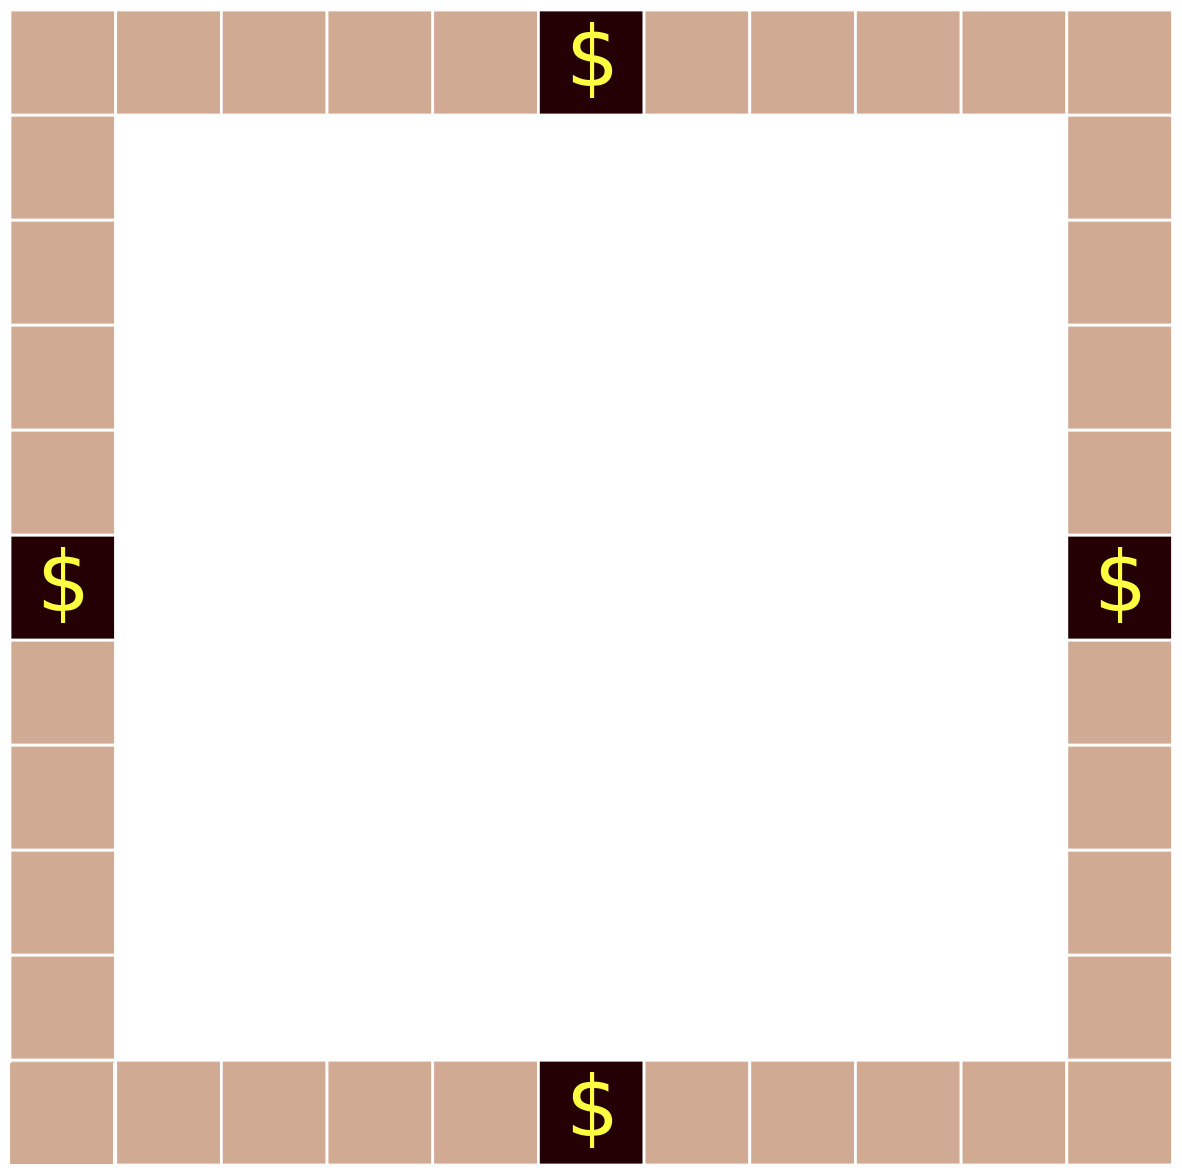
\includegraphics[width=0.19\textwidth]{figures/lgw/env.png}}
    \subfigure[HalfCheetah]{\label{fig:hc}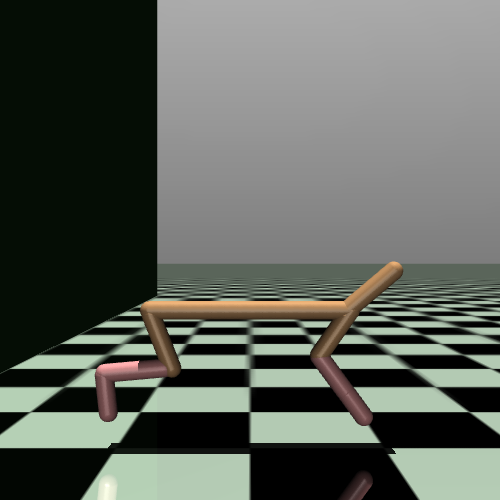
\includegraphics[width=0.19\textwidth]{figures/hc/env.png}}
    \subfigure[Ant]{\label{fig:ant}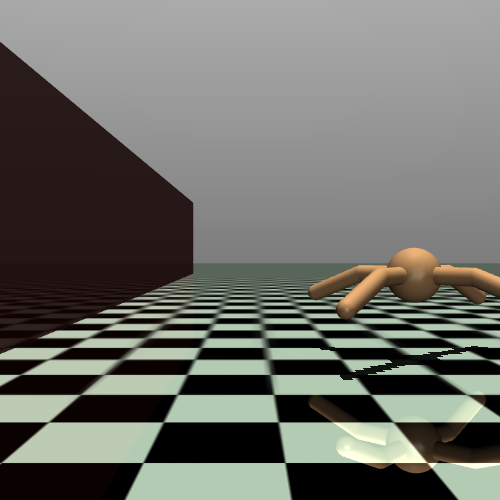
\includegraphics[width=0.19\textwidth]{figures/ant/env.png}}
    % \subfigure[Point]{\label{fig:point}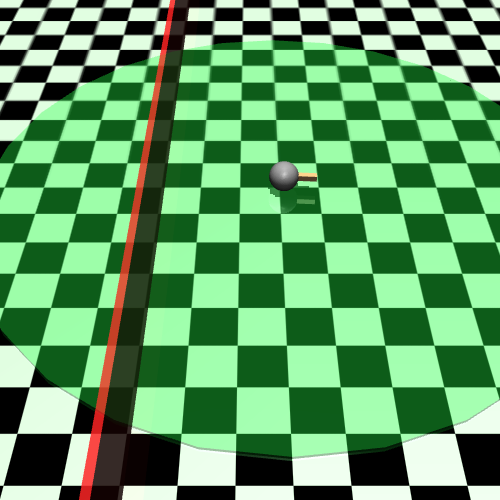
\includegraphics[width=0.19\textwidth]{figures/point/env.png}}
    % \subfigure[AntBroken]{\label{fig:ant-broken}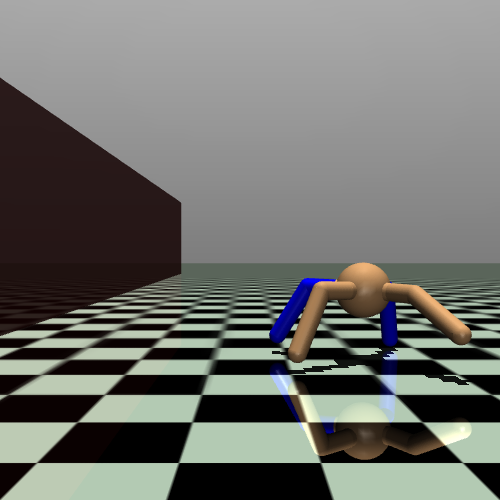
\includegraphics[width=0.19\textwidth]{figures/ant_broken/env.png}}
    \caption{The environments used in the experiments for learning constraints.}
    \label{fig:envs}
\end{center}
\vskip -0.2in
\end{figure}
\end{frame}

\begin{frame}[fragile]{Results: Learning Constraints}
\begin{figure}
% \vskip 0.2in
\begin{center}
    \small{\bfseries Reward (higher is better):}\\
    \subfigure{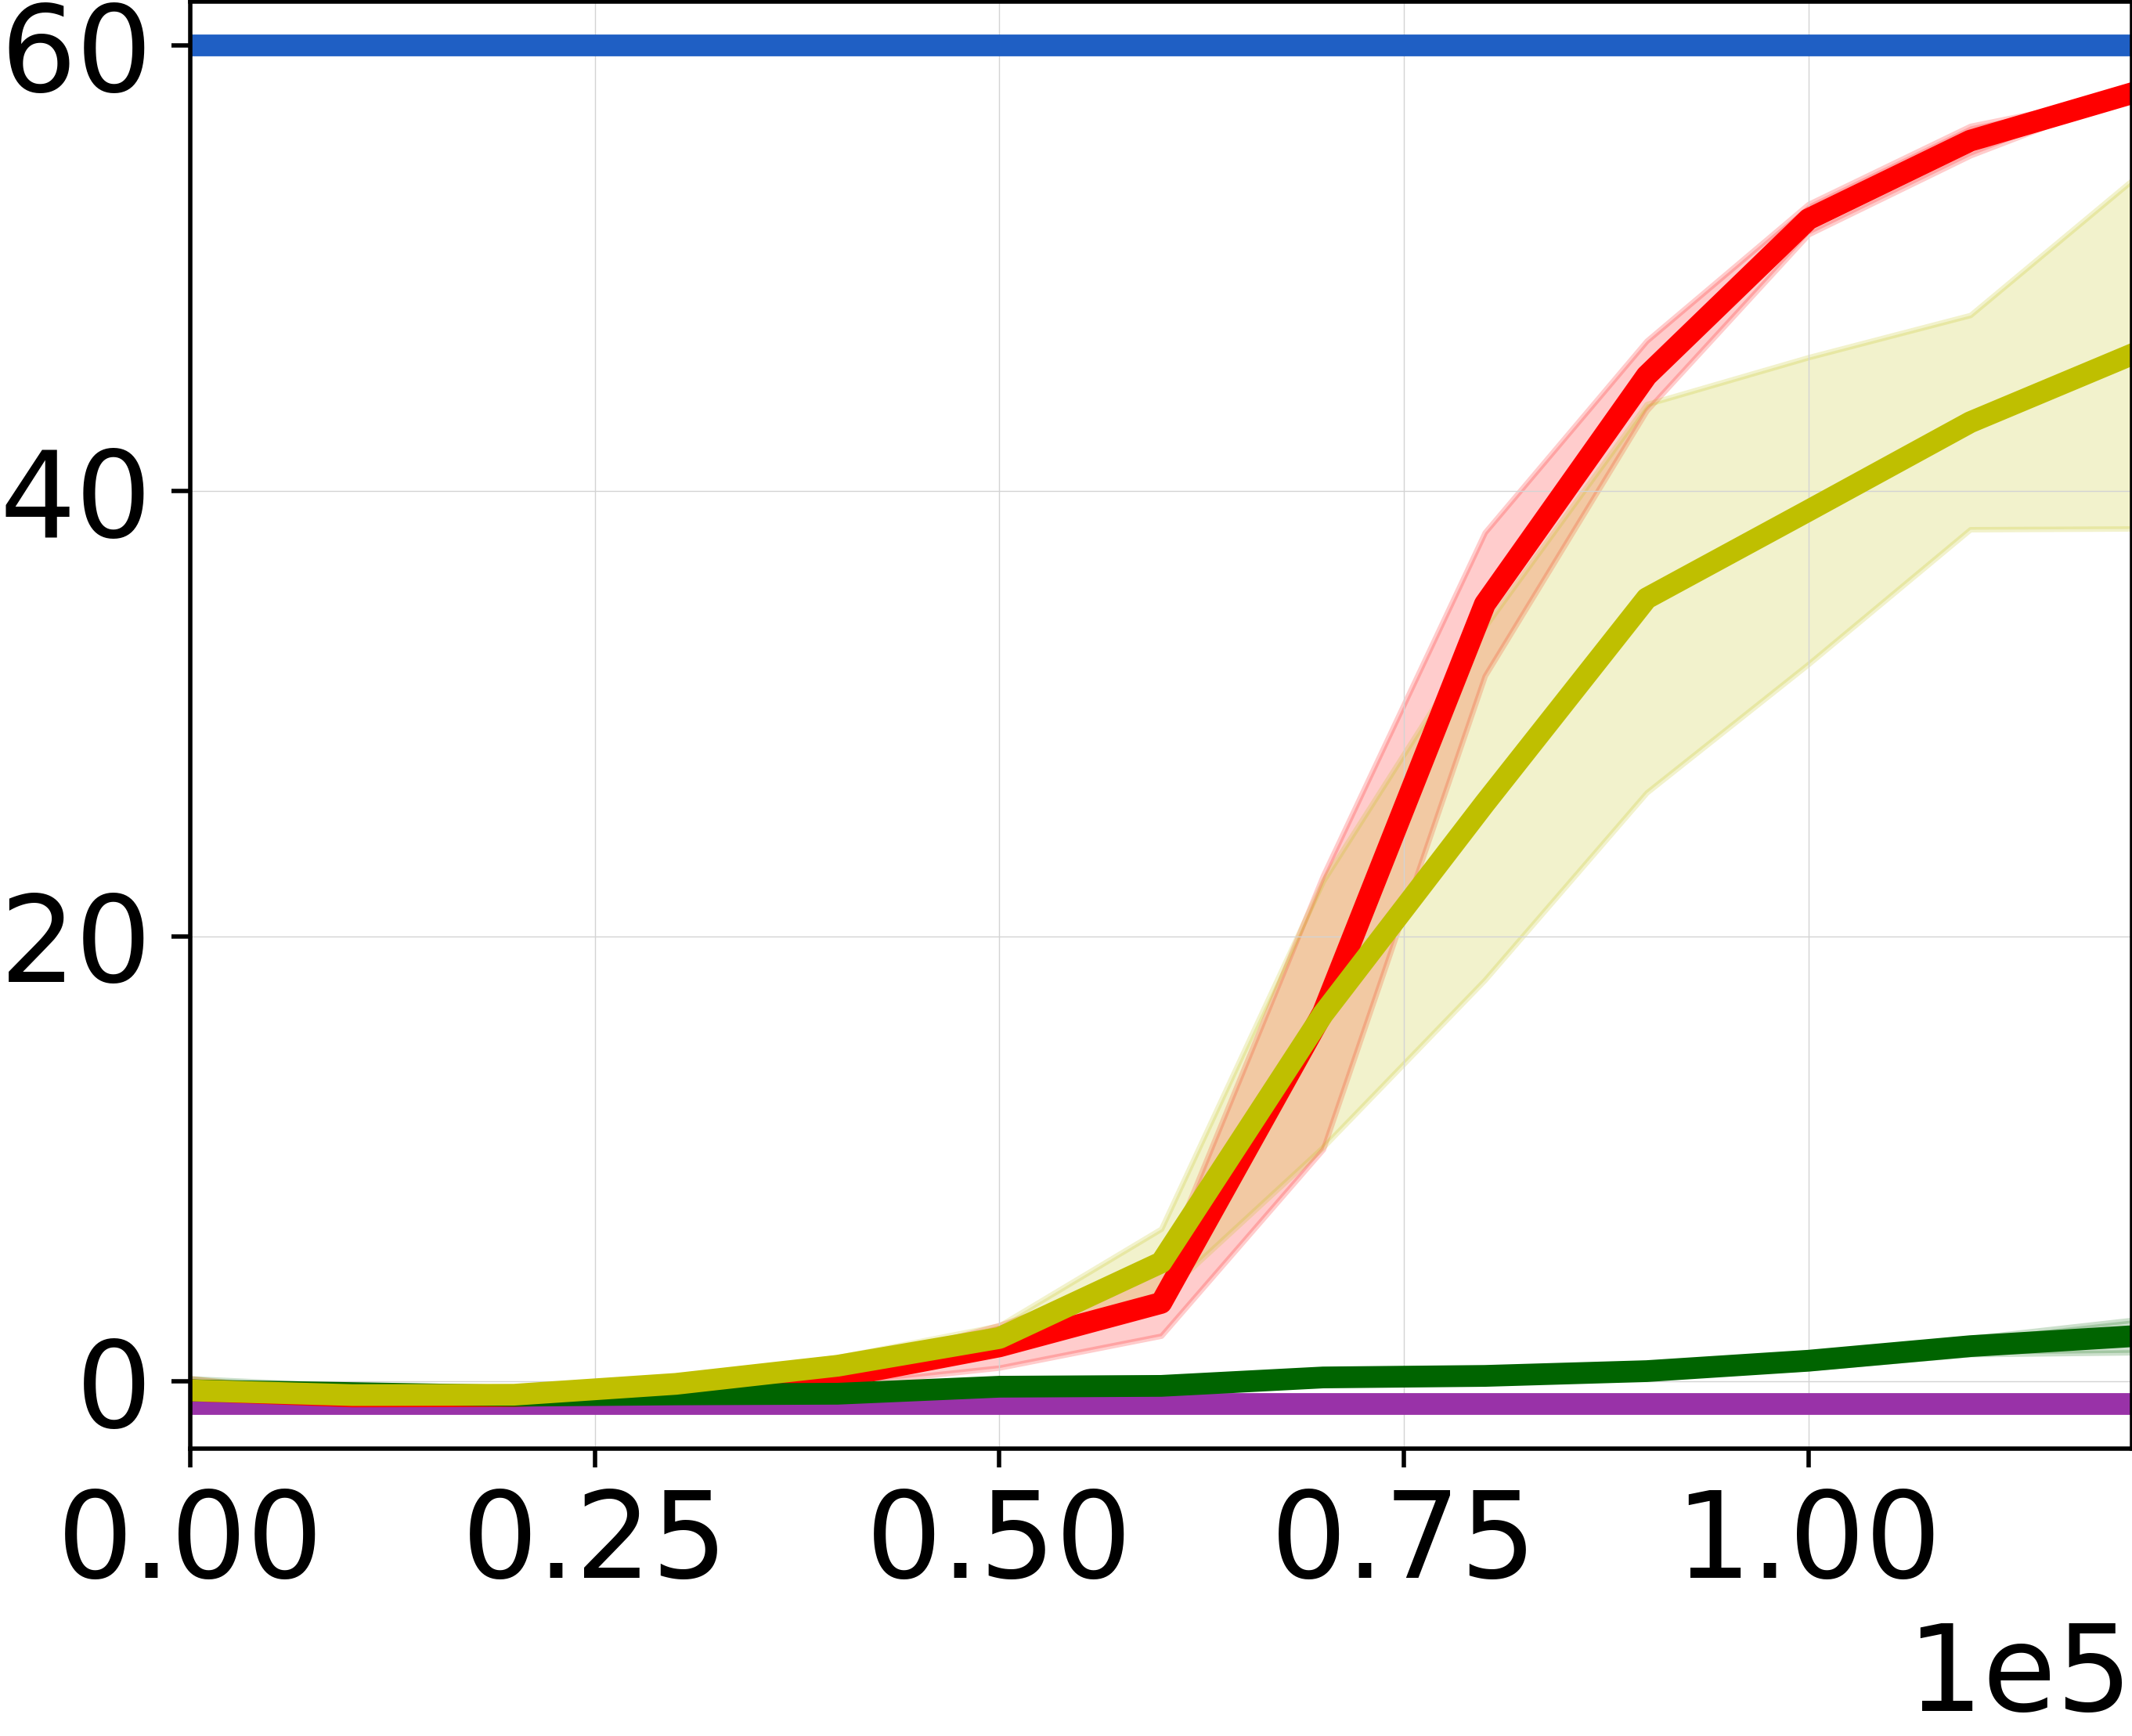
\includegraphics[width=0.18\textwidth]{figures/lgw/reward.png}}\hspace{0.2in}
    \subfigure{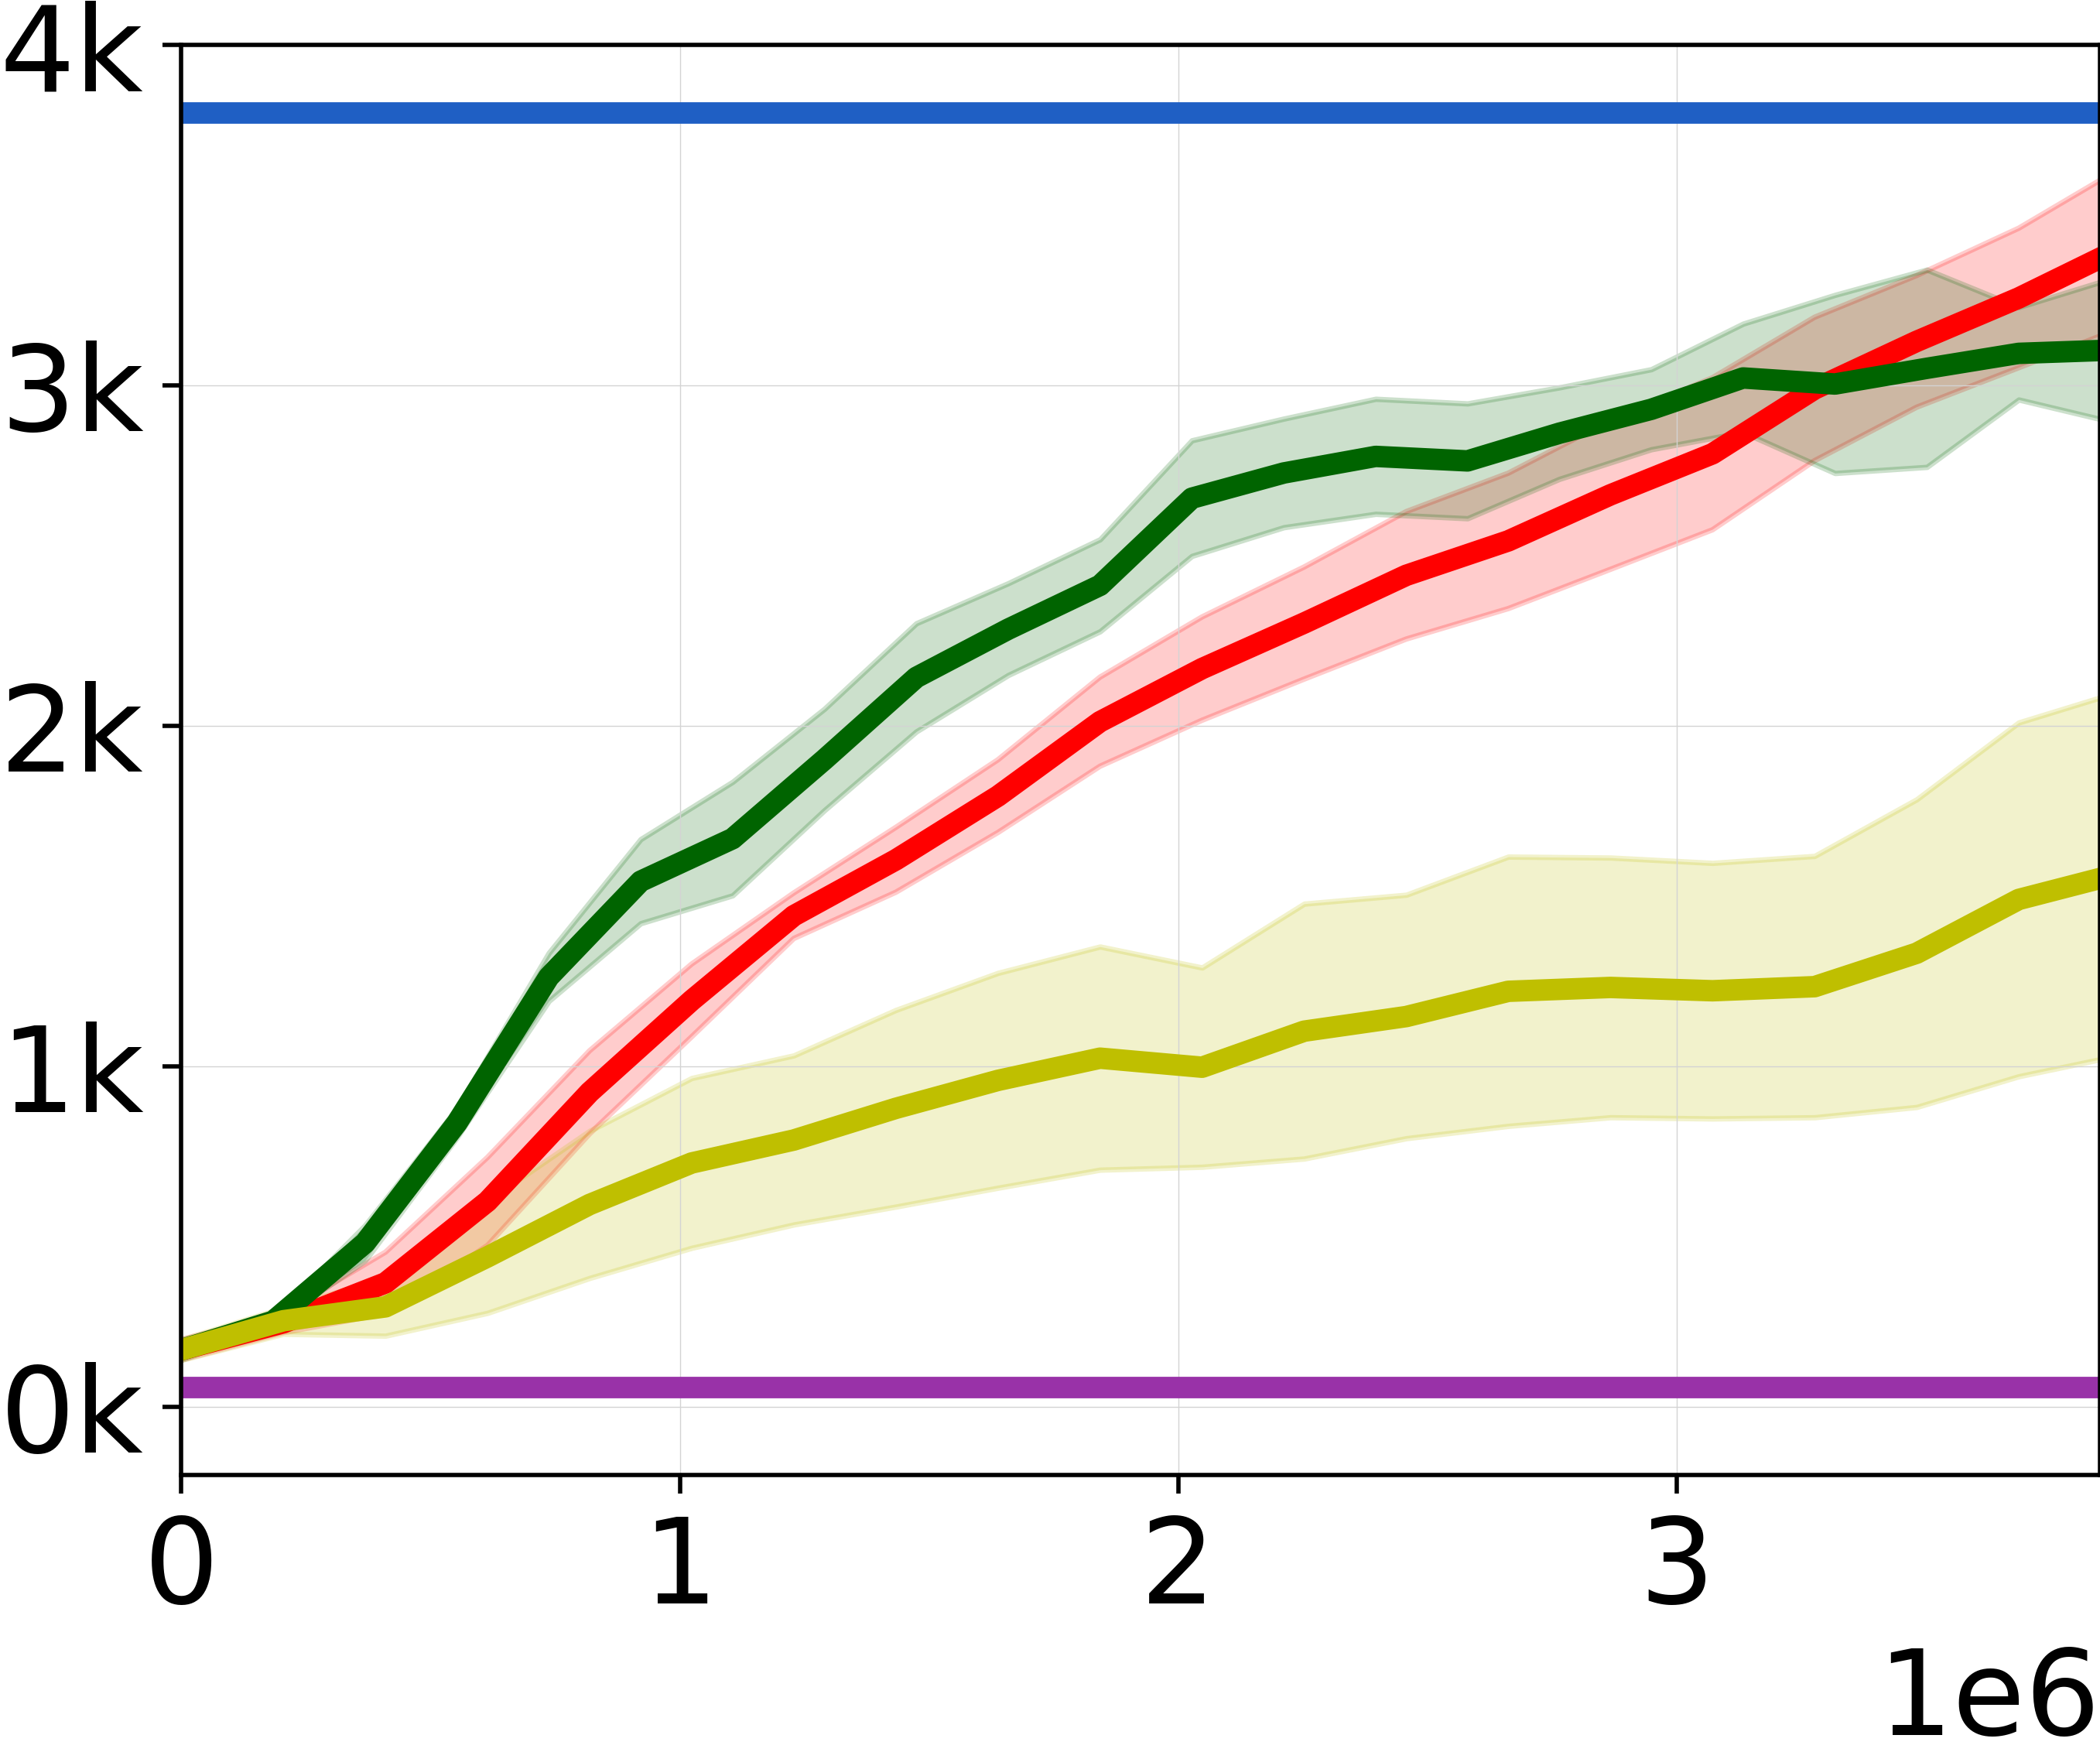
\includegraphics[width=0.18\textwidth]{figures/hc/reward.png}}\hspace{0.2in}
    \subfigure{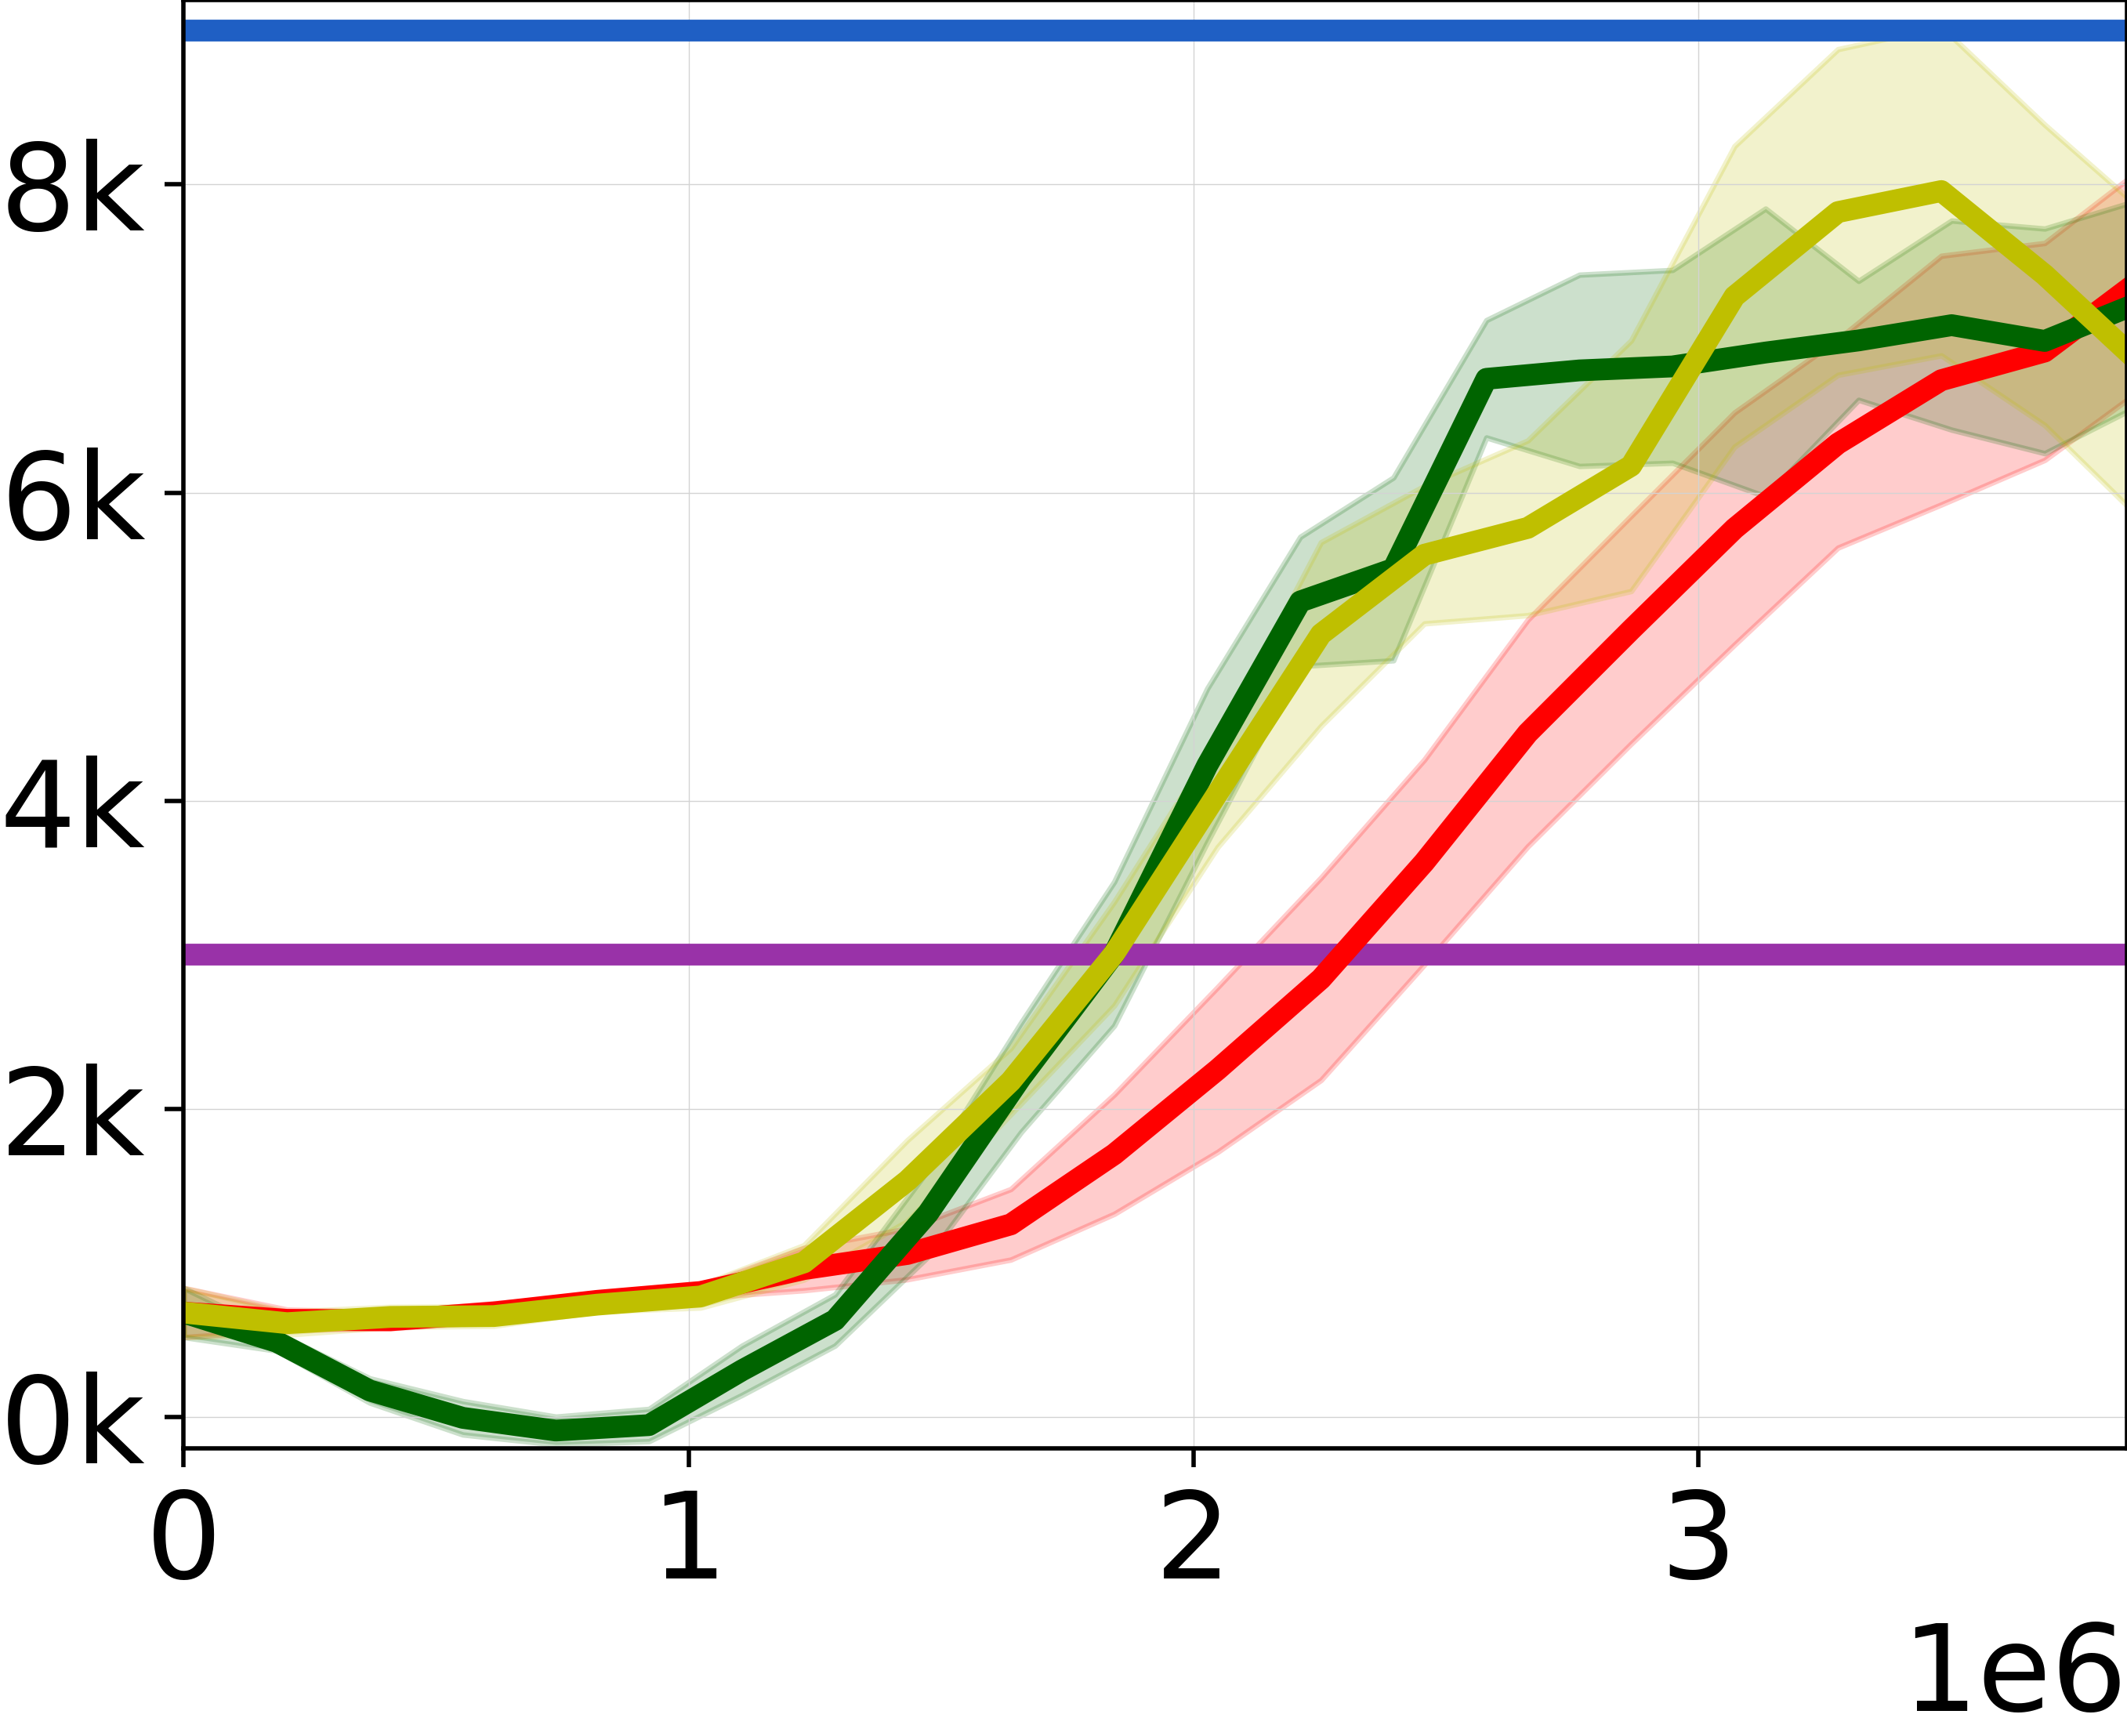
\includegraphics[width=0.18\textwidth]{figures/ant/reward.png}}\\
    \setcounter{subfigure}{0}
    \small{\bfseries Constraint violations (lower is better):}\\
    \subfigure[LapGridWorld]{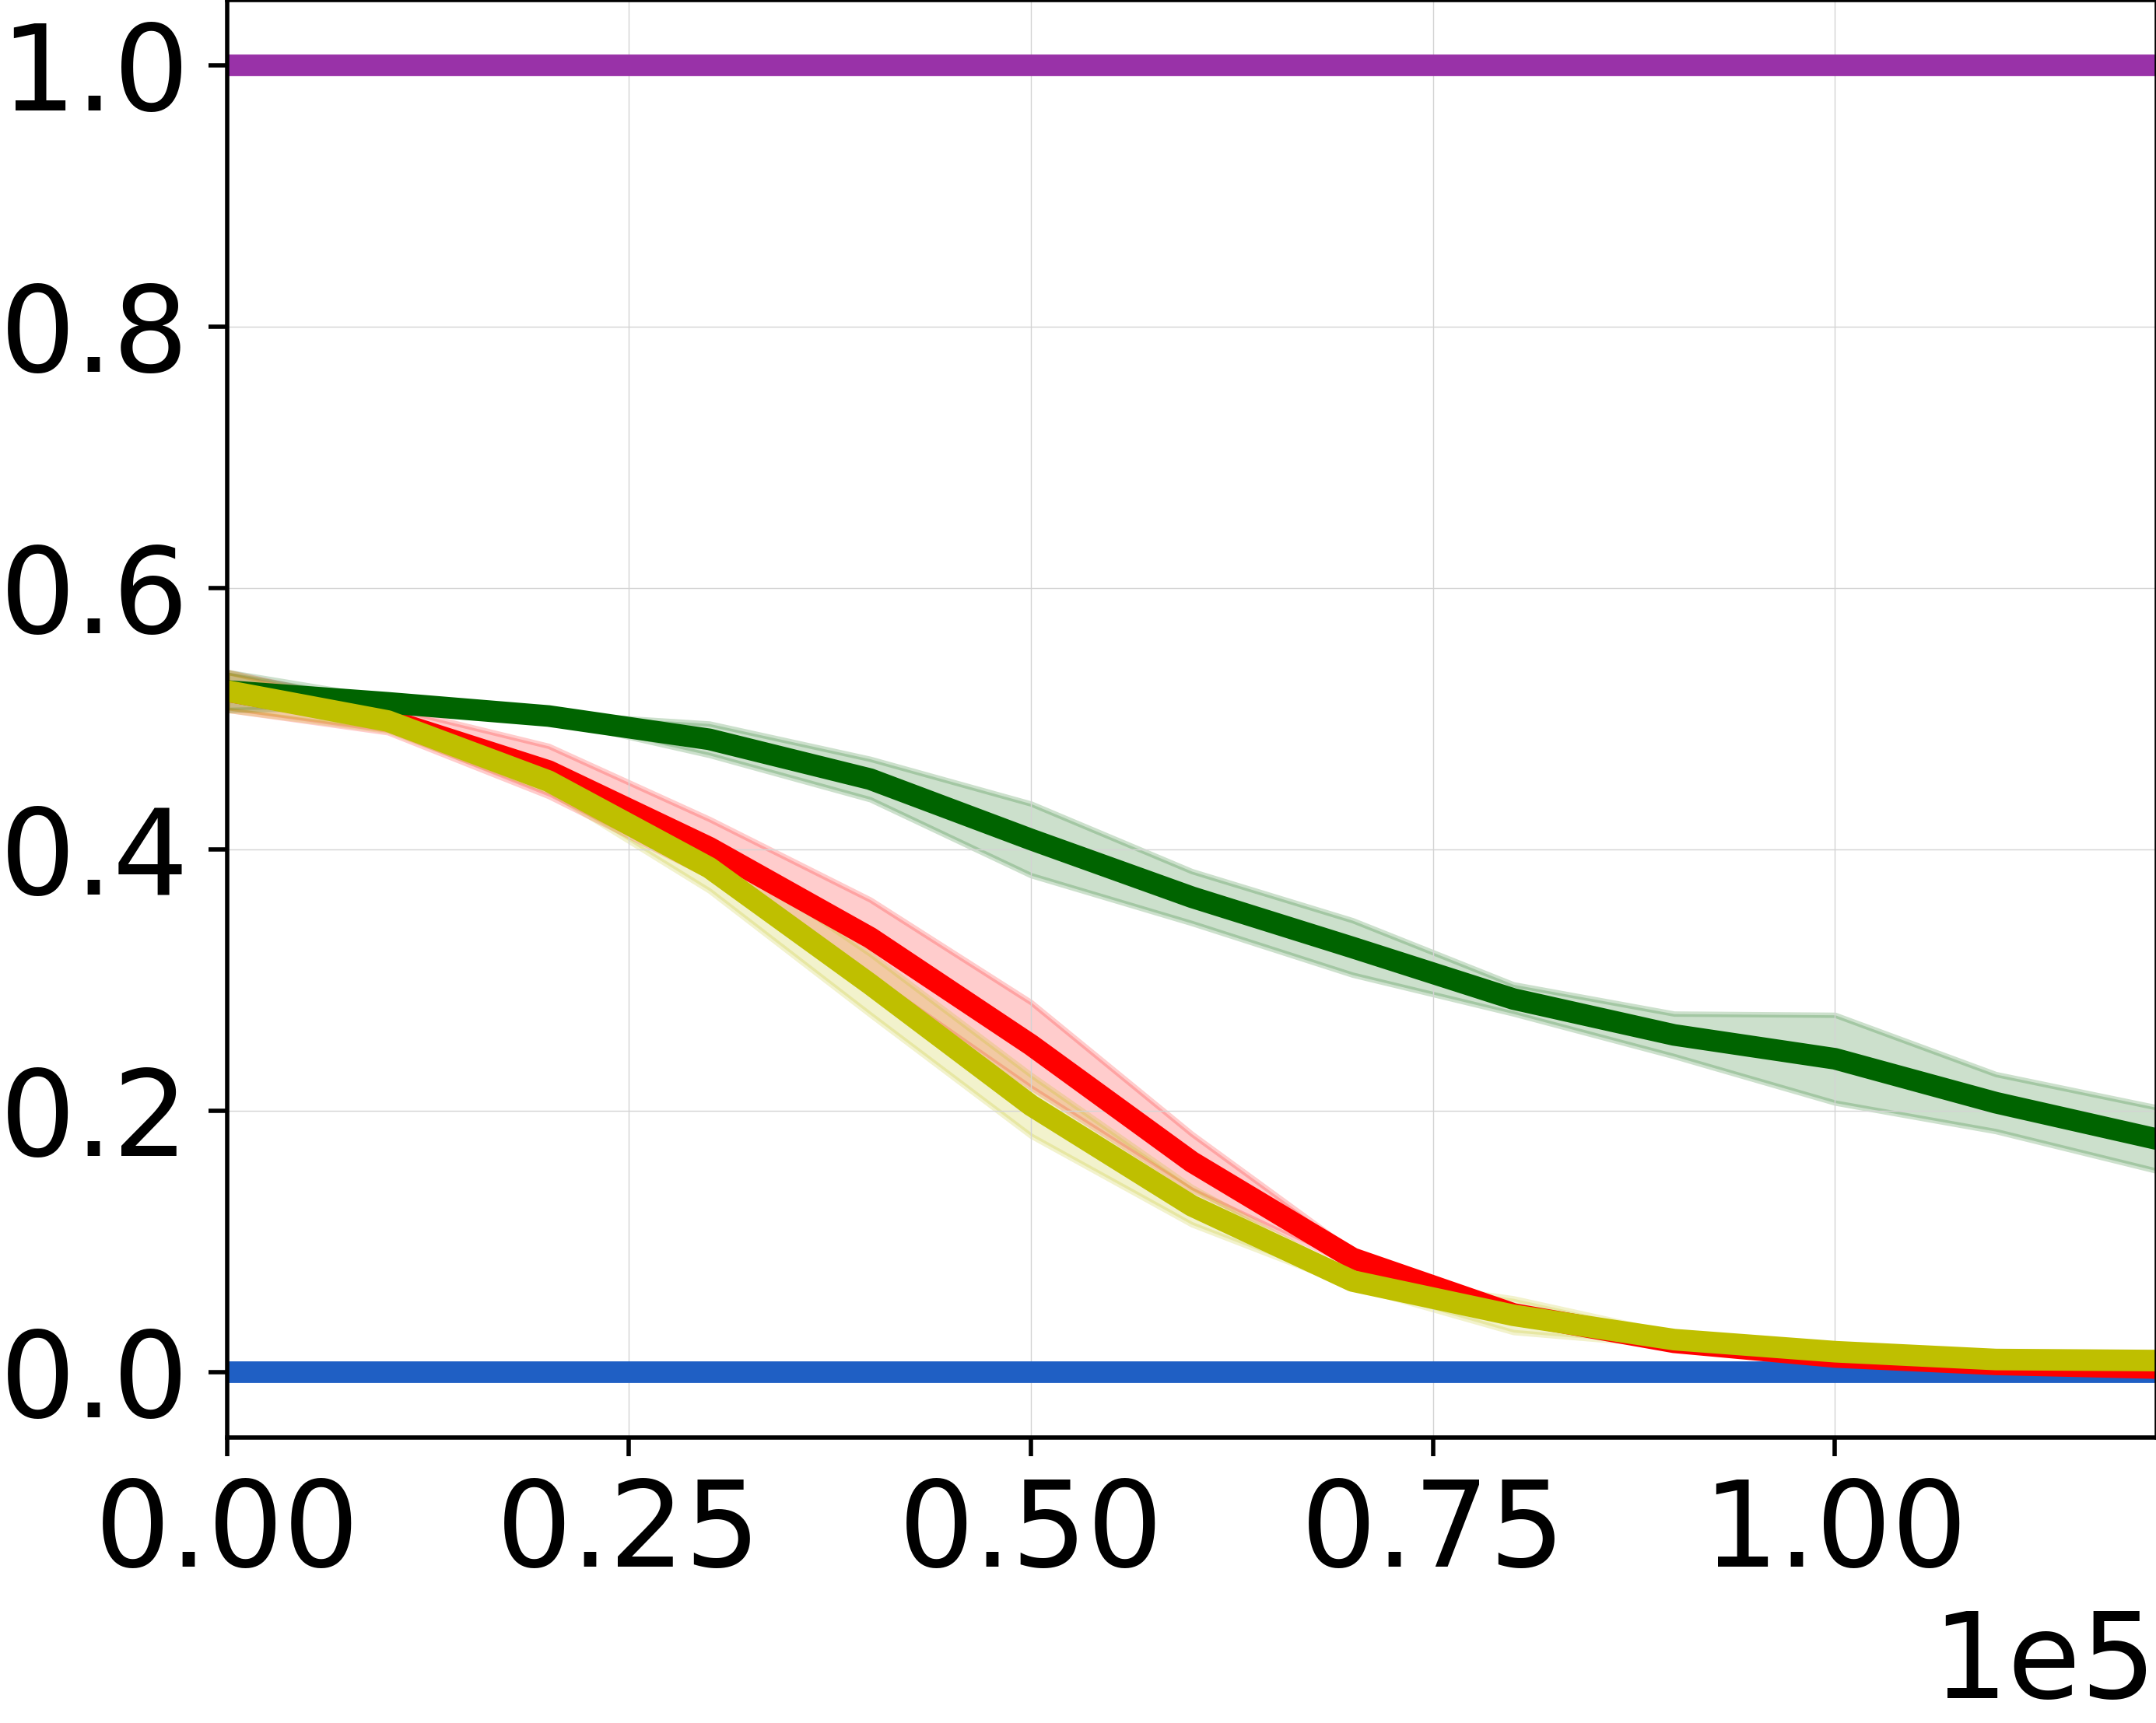
\includegraphics[width=0.18\textwidth]{figures/lgw/violations.png}}\hspace{0.2in}
    \subfigure[HalfCheetah]{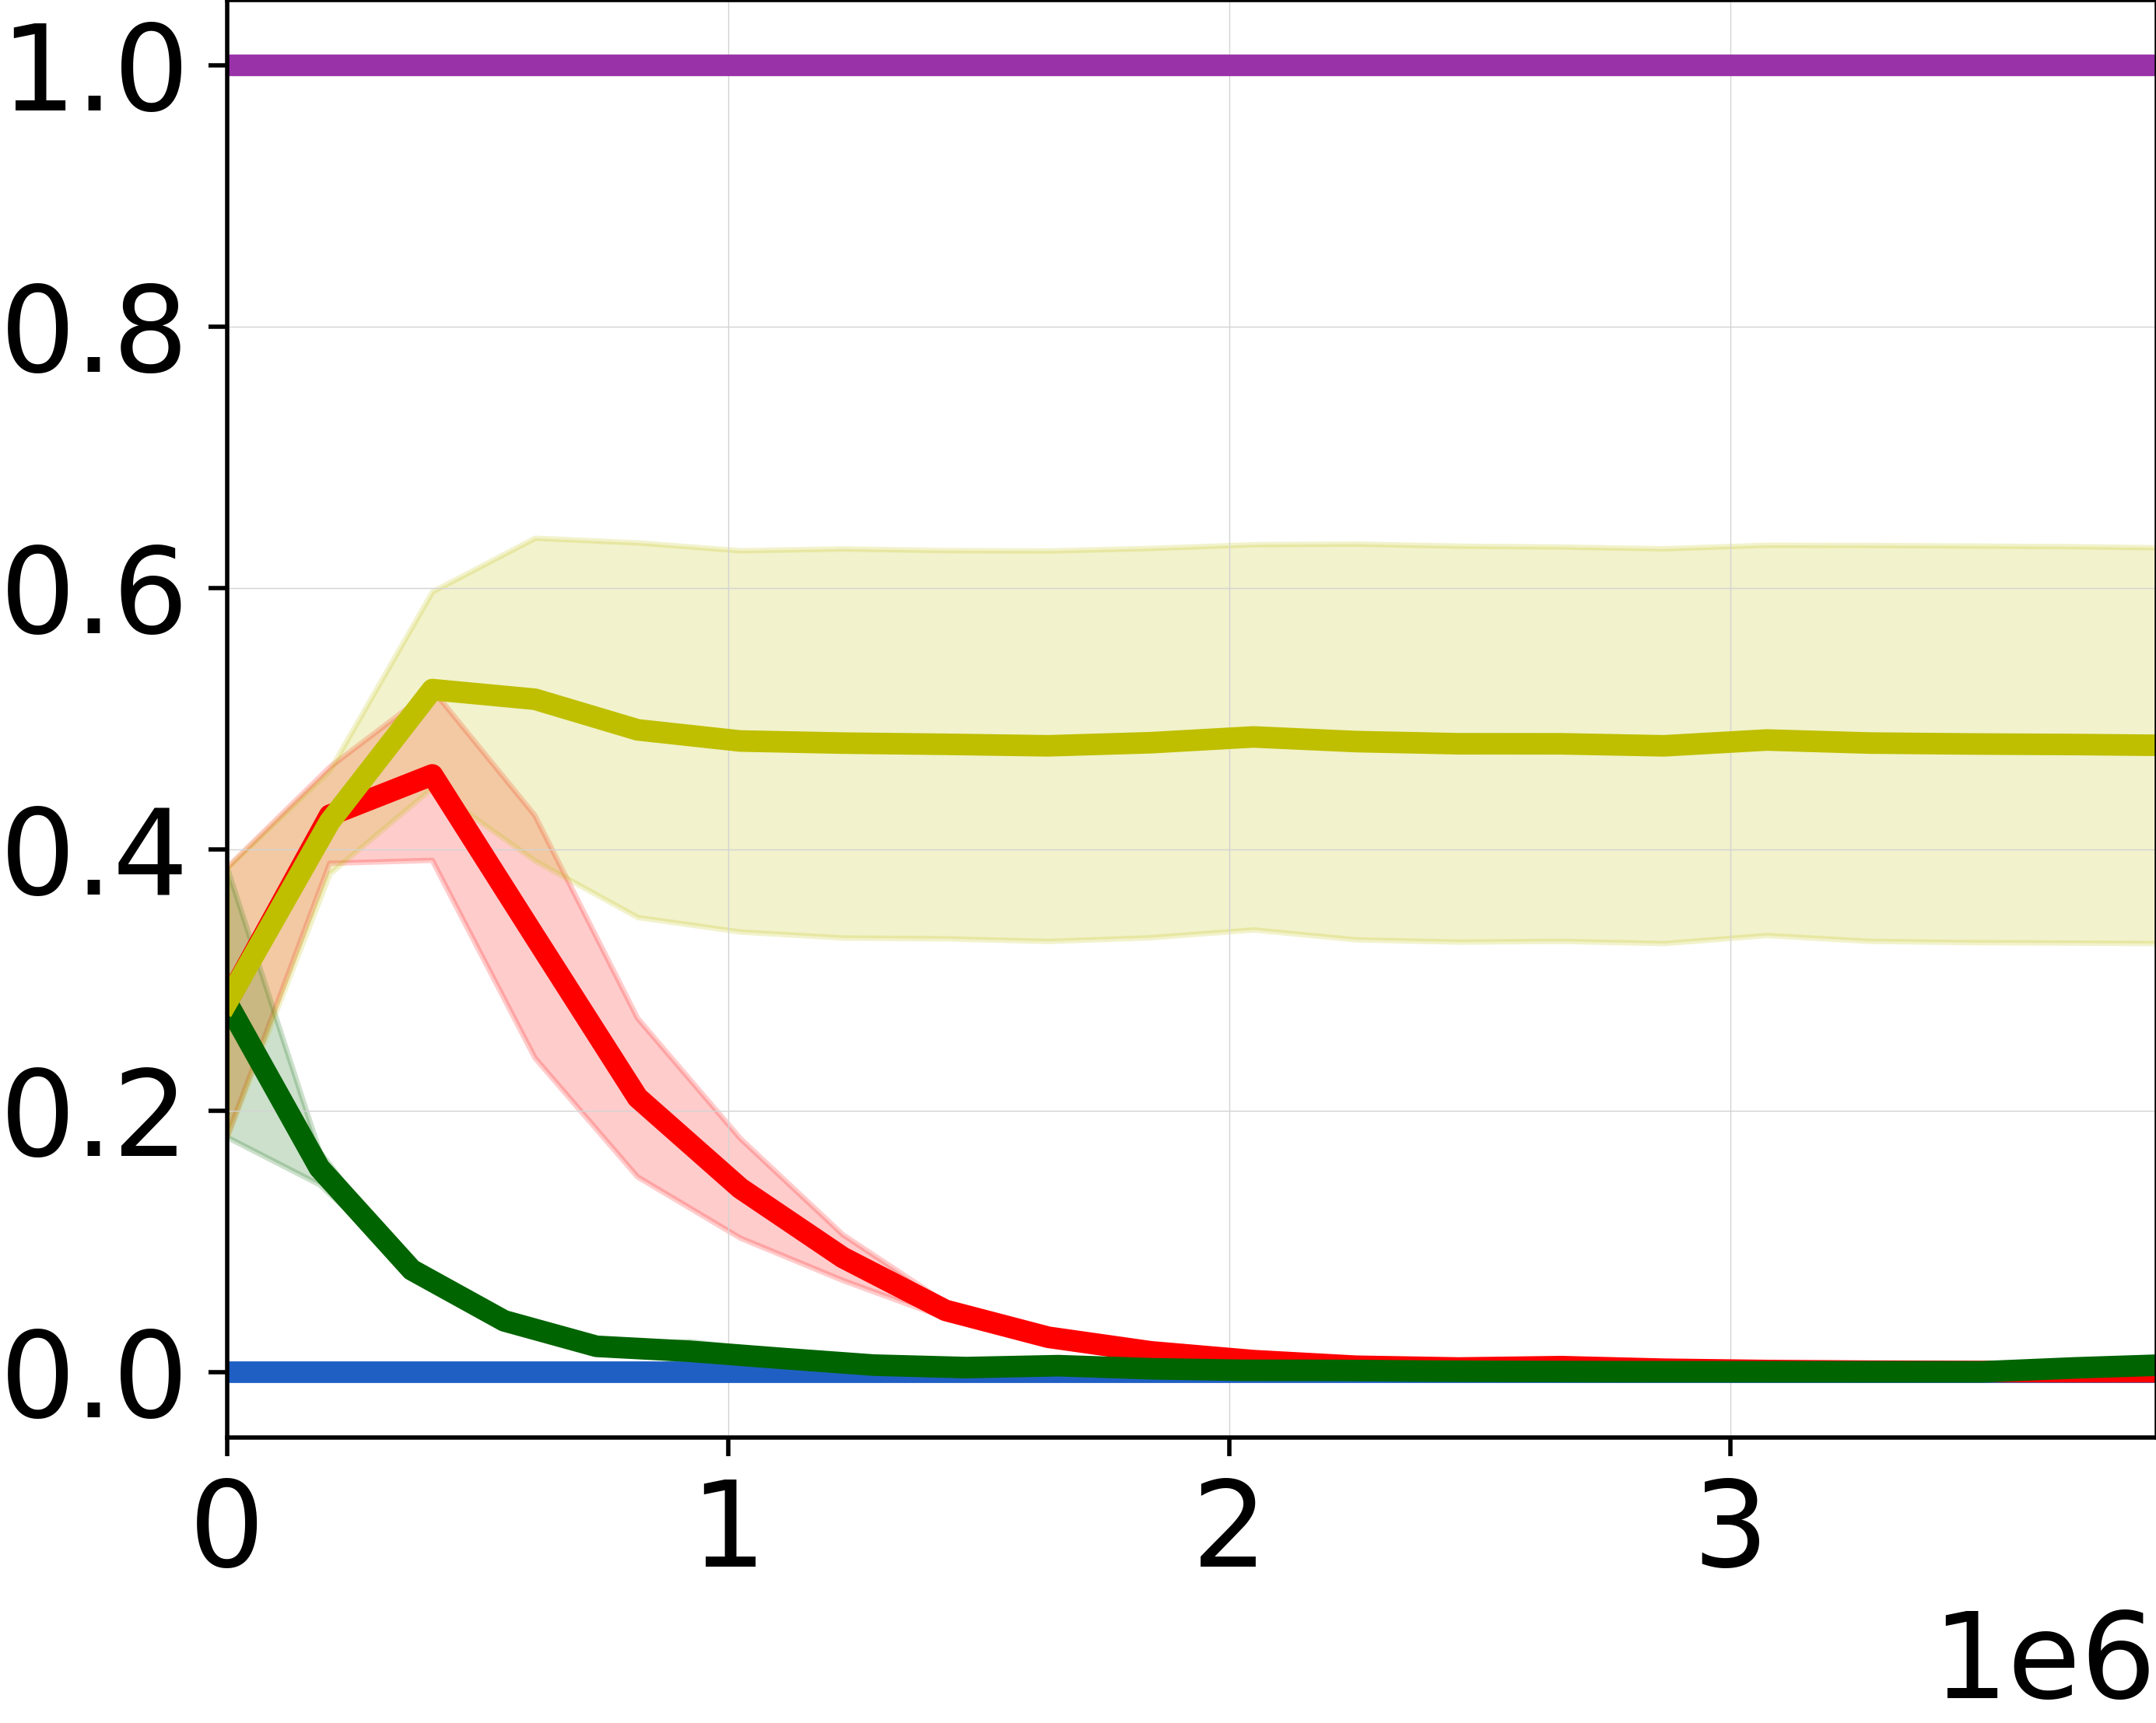
\includegraphics[width=0.18\textwidth]{figures/hc/violations.png}}\hspace{0.2in}
    \subfigure[Ant]{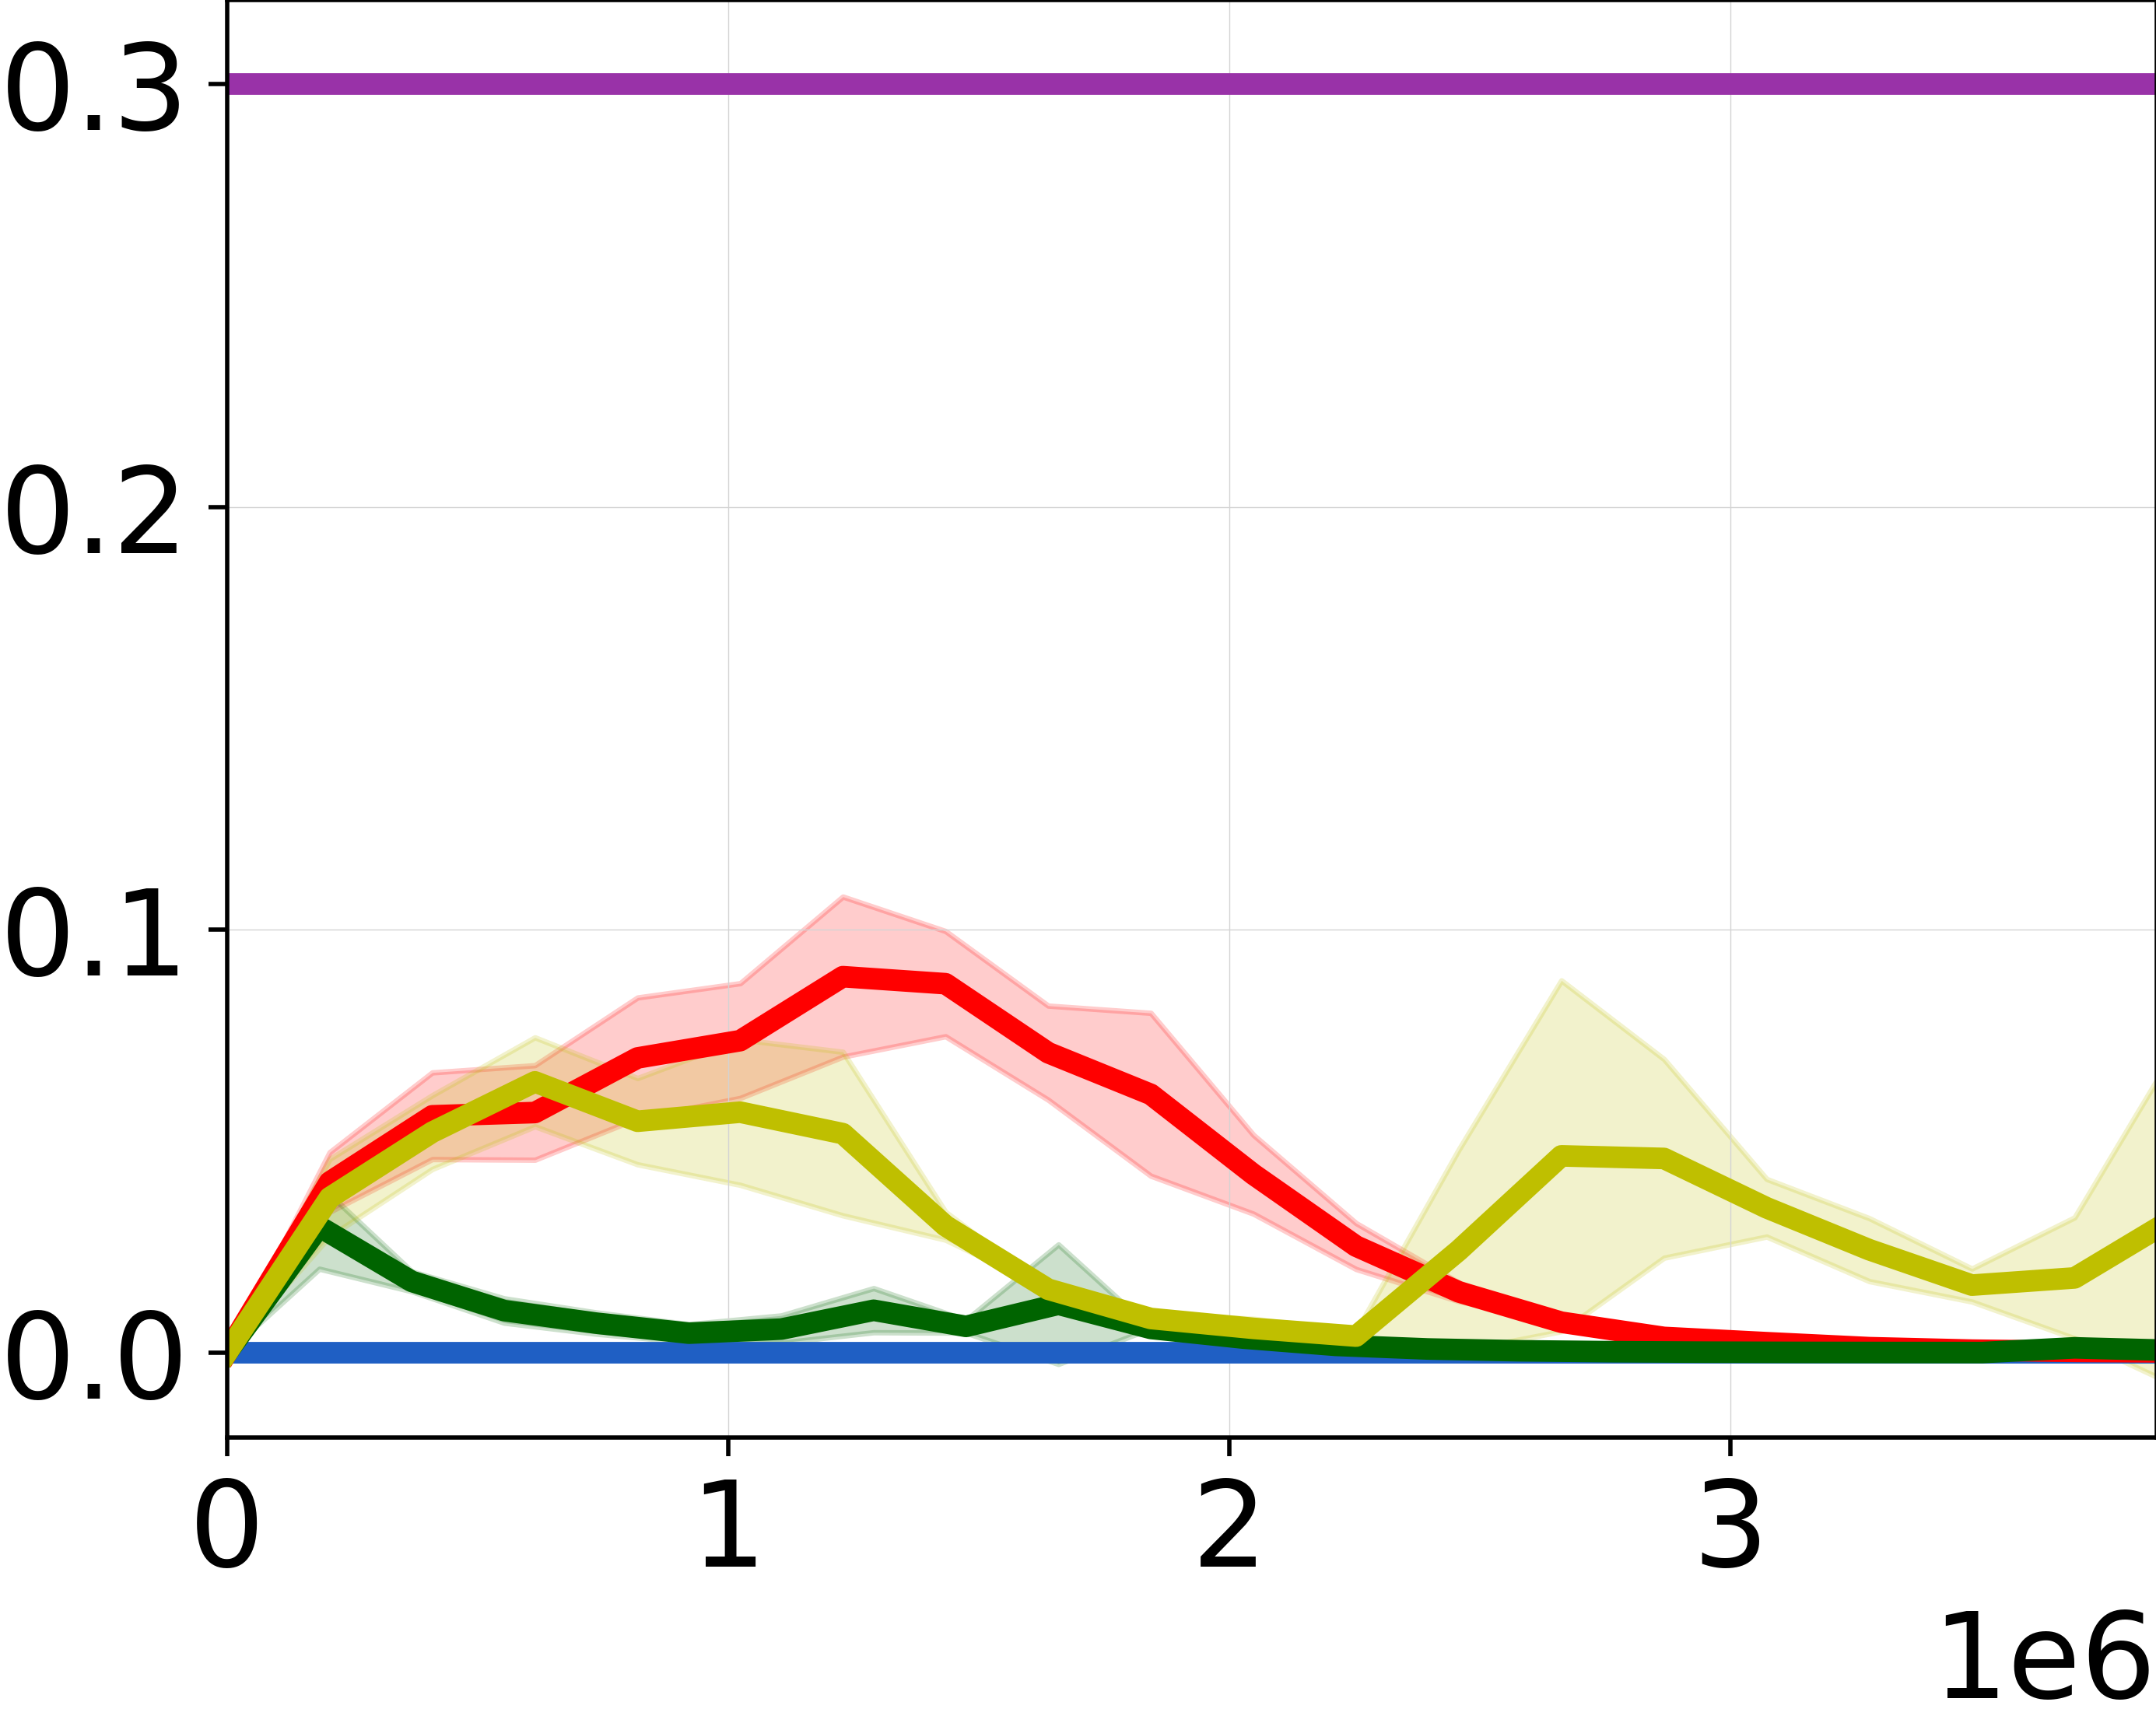
\includegraphics[width=0.18\textwidth]{figures/ant/violations.png}}
    \subfigure{
\includegraphics[width=0.6\textwidth]{figures/legend.png}}\\
    \caption{\tiny{Performance of agents during training over several seeds (5 in LapGridWorld, 10 in others). The x-axis is the number of timesteps taken in the environment. The shaded regions correspond to the standard error.}}
    \label{fig:main_results}
\end{center}
% \vskip -0.2in
\end{figure}
\end{frame}



\begin{frame}{Results: Transferring Constraints}
\begin{figure}
\vskip 0.4in
% \begin{center}
    \subfigure[Ant]{\label{fig:ant2}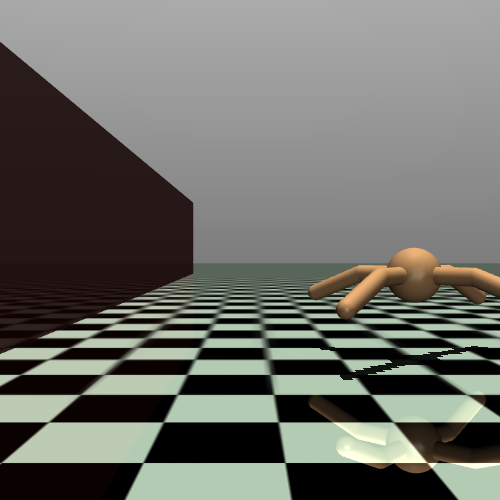
\includegraphics[width=0.19\textwidth]{figures/ant/env.png}}
    % \hspace{15pt}
    {\label{fig:arrow}
\includegraphics[width=0.19\textwidth]{figures/rightarrow.jpg}}
    % \hspace{15pt}
    \subfigure[Point]{\label{fig:point2}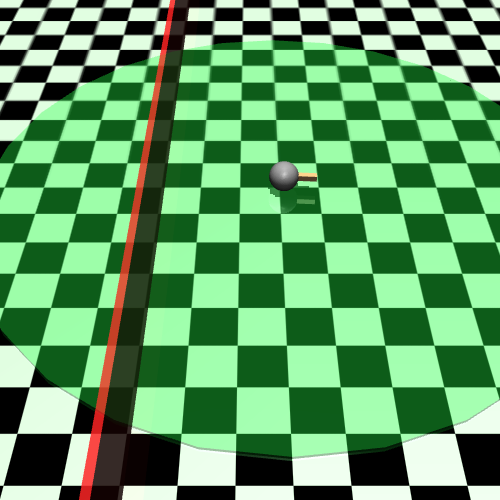
\includegraphics[width=0.19\textwidth]{figures/point/env.png}}
    \subfigure[AntBroken]{\label{fig:ant-broken}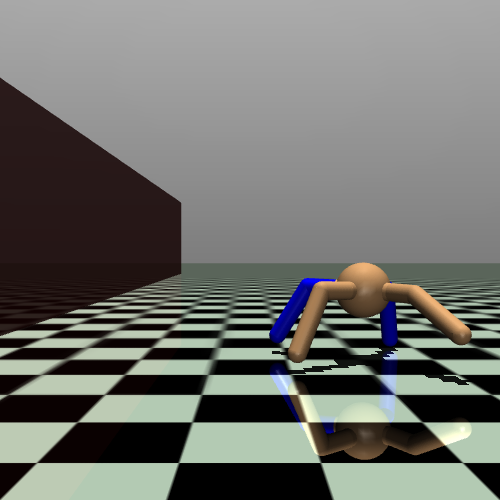
\includegraphics[width=0.19\textwidth]{figures/ant_broken/env.png}}
    \caption{Constraints learned in ant environment were transferred to point and ant broken environments.}
    \label{fig:envs2}
% \end{center}
\vskip -0.2in
\end{figure}
\end{frame}

\begin{frame}{Results: Transferring Constraints}
\begin{figure}
\begin{center}
    \subfigure{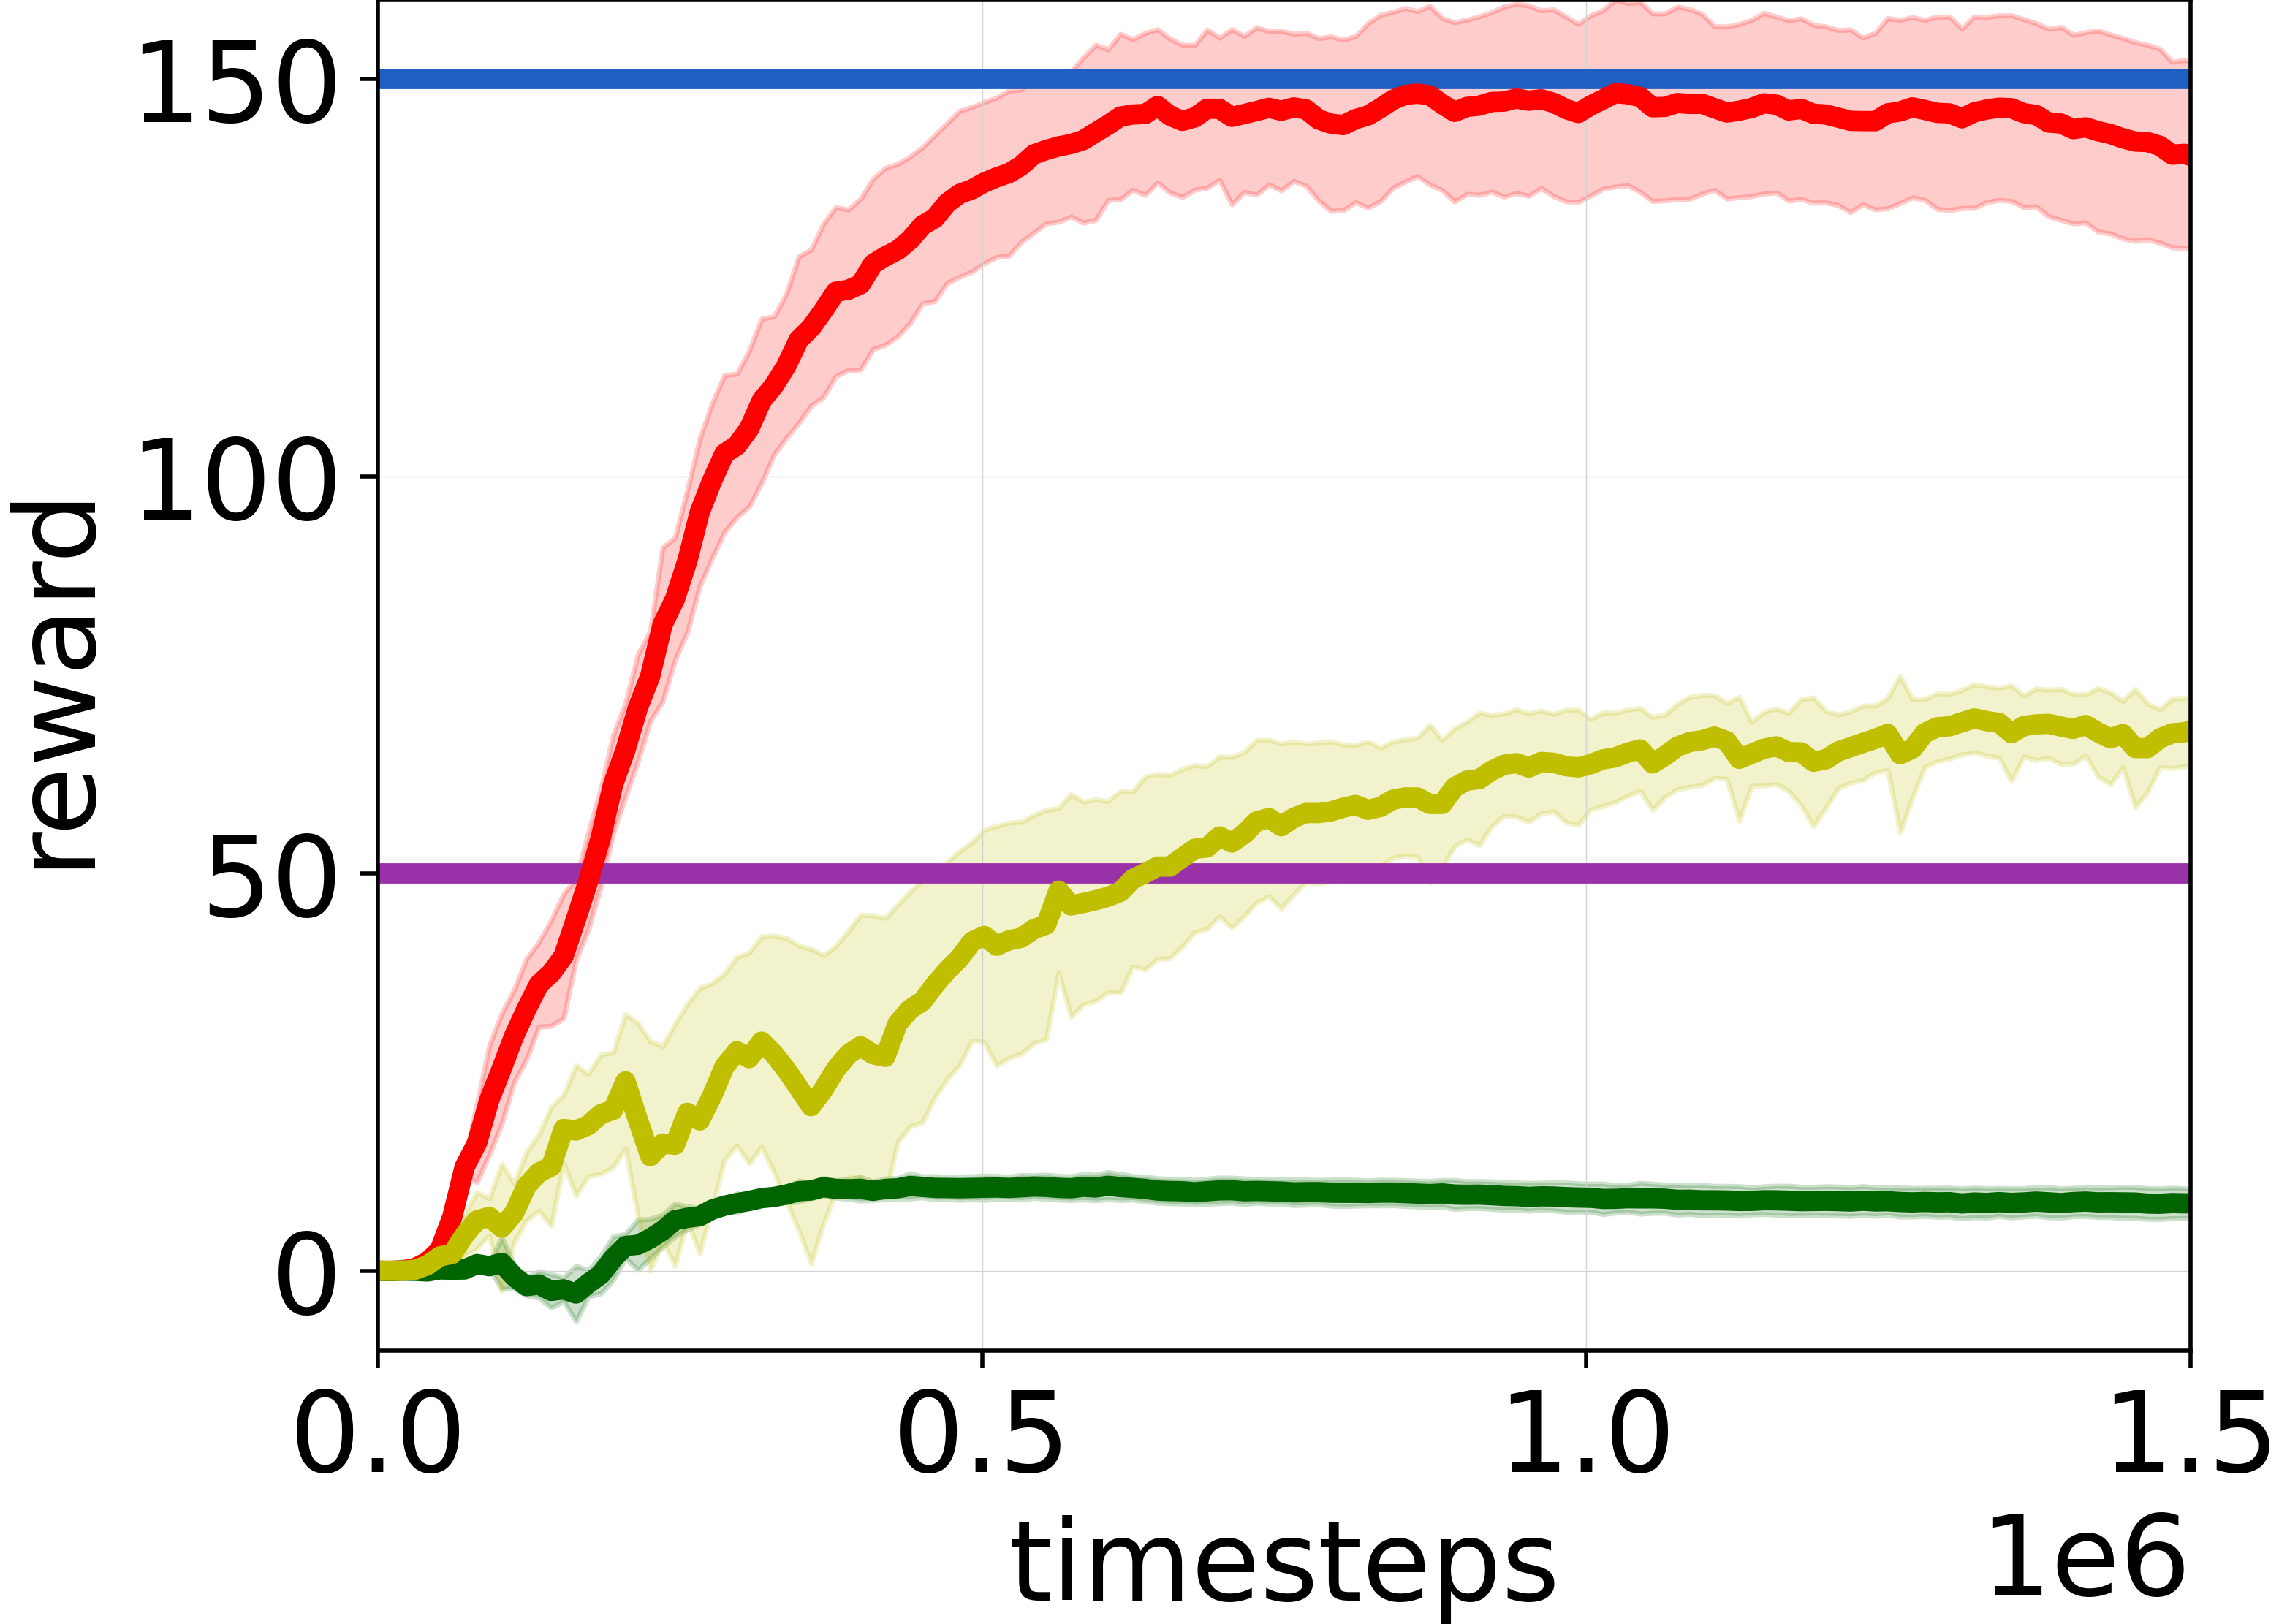
\includegraphics[width=0.20\columnwidth]{figures/point/reward.png}}
    \subfigure{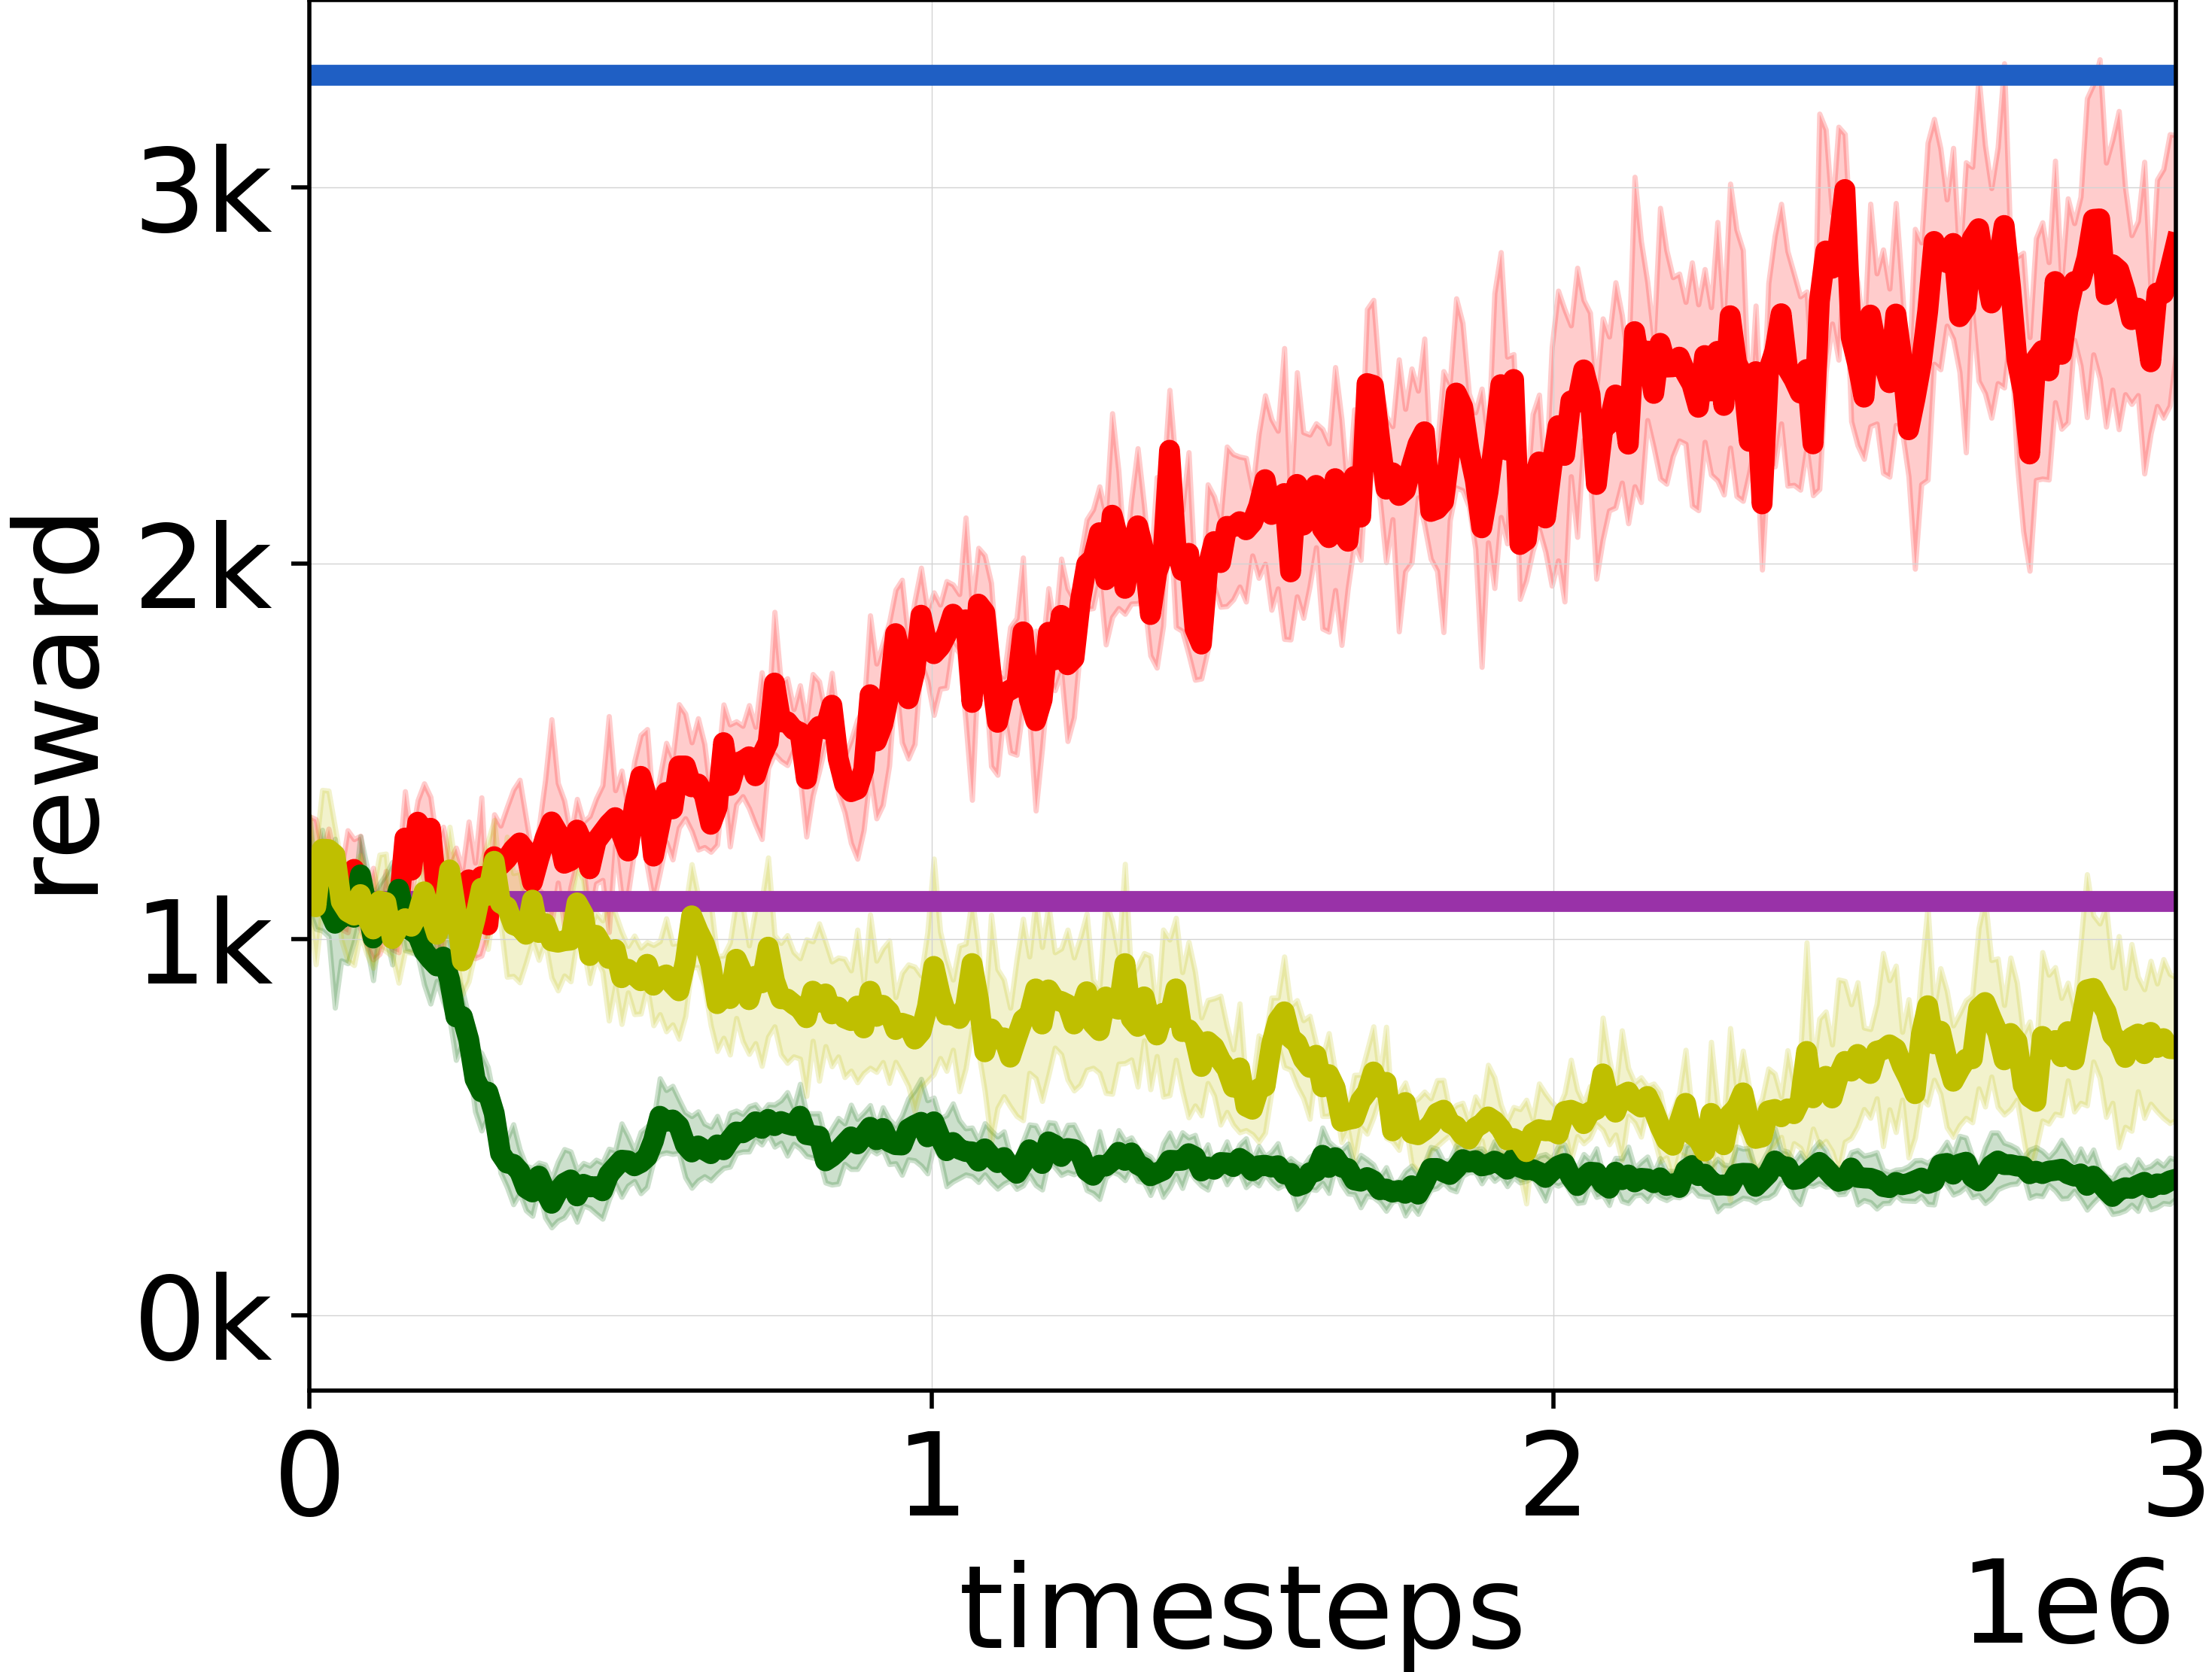
\includegraphics[width=0.20\columnwidth]{figures/ant_broken/reward.png}}\\
    \setcounter{subfigure}{0}
    \subfigure[Point]{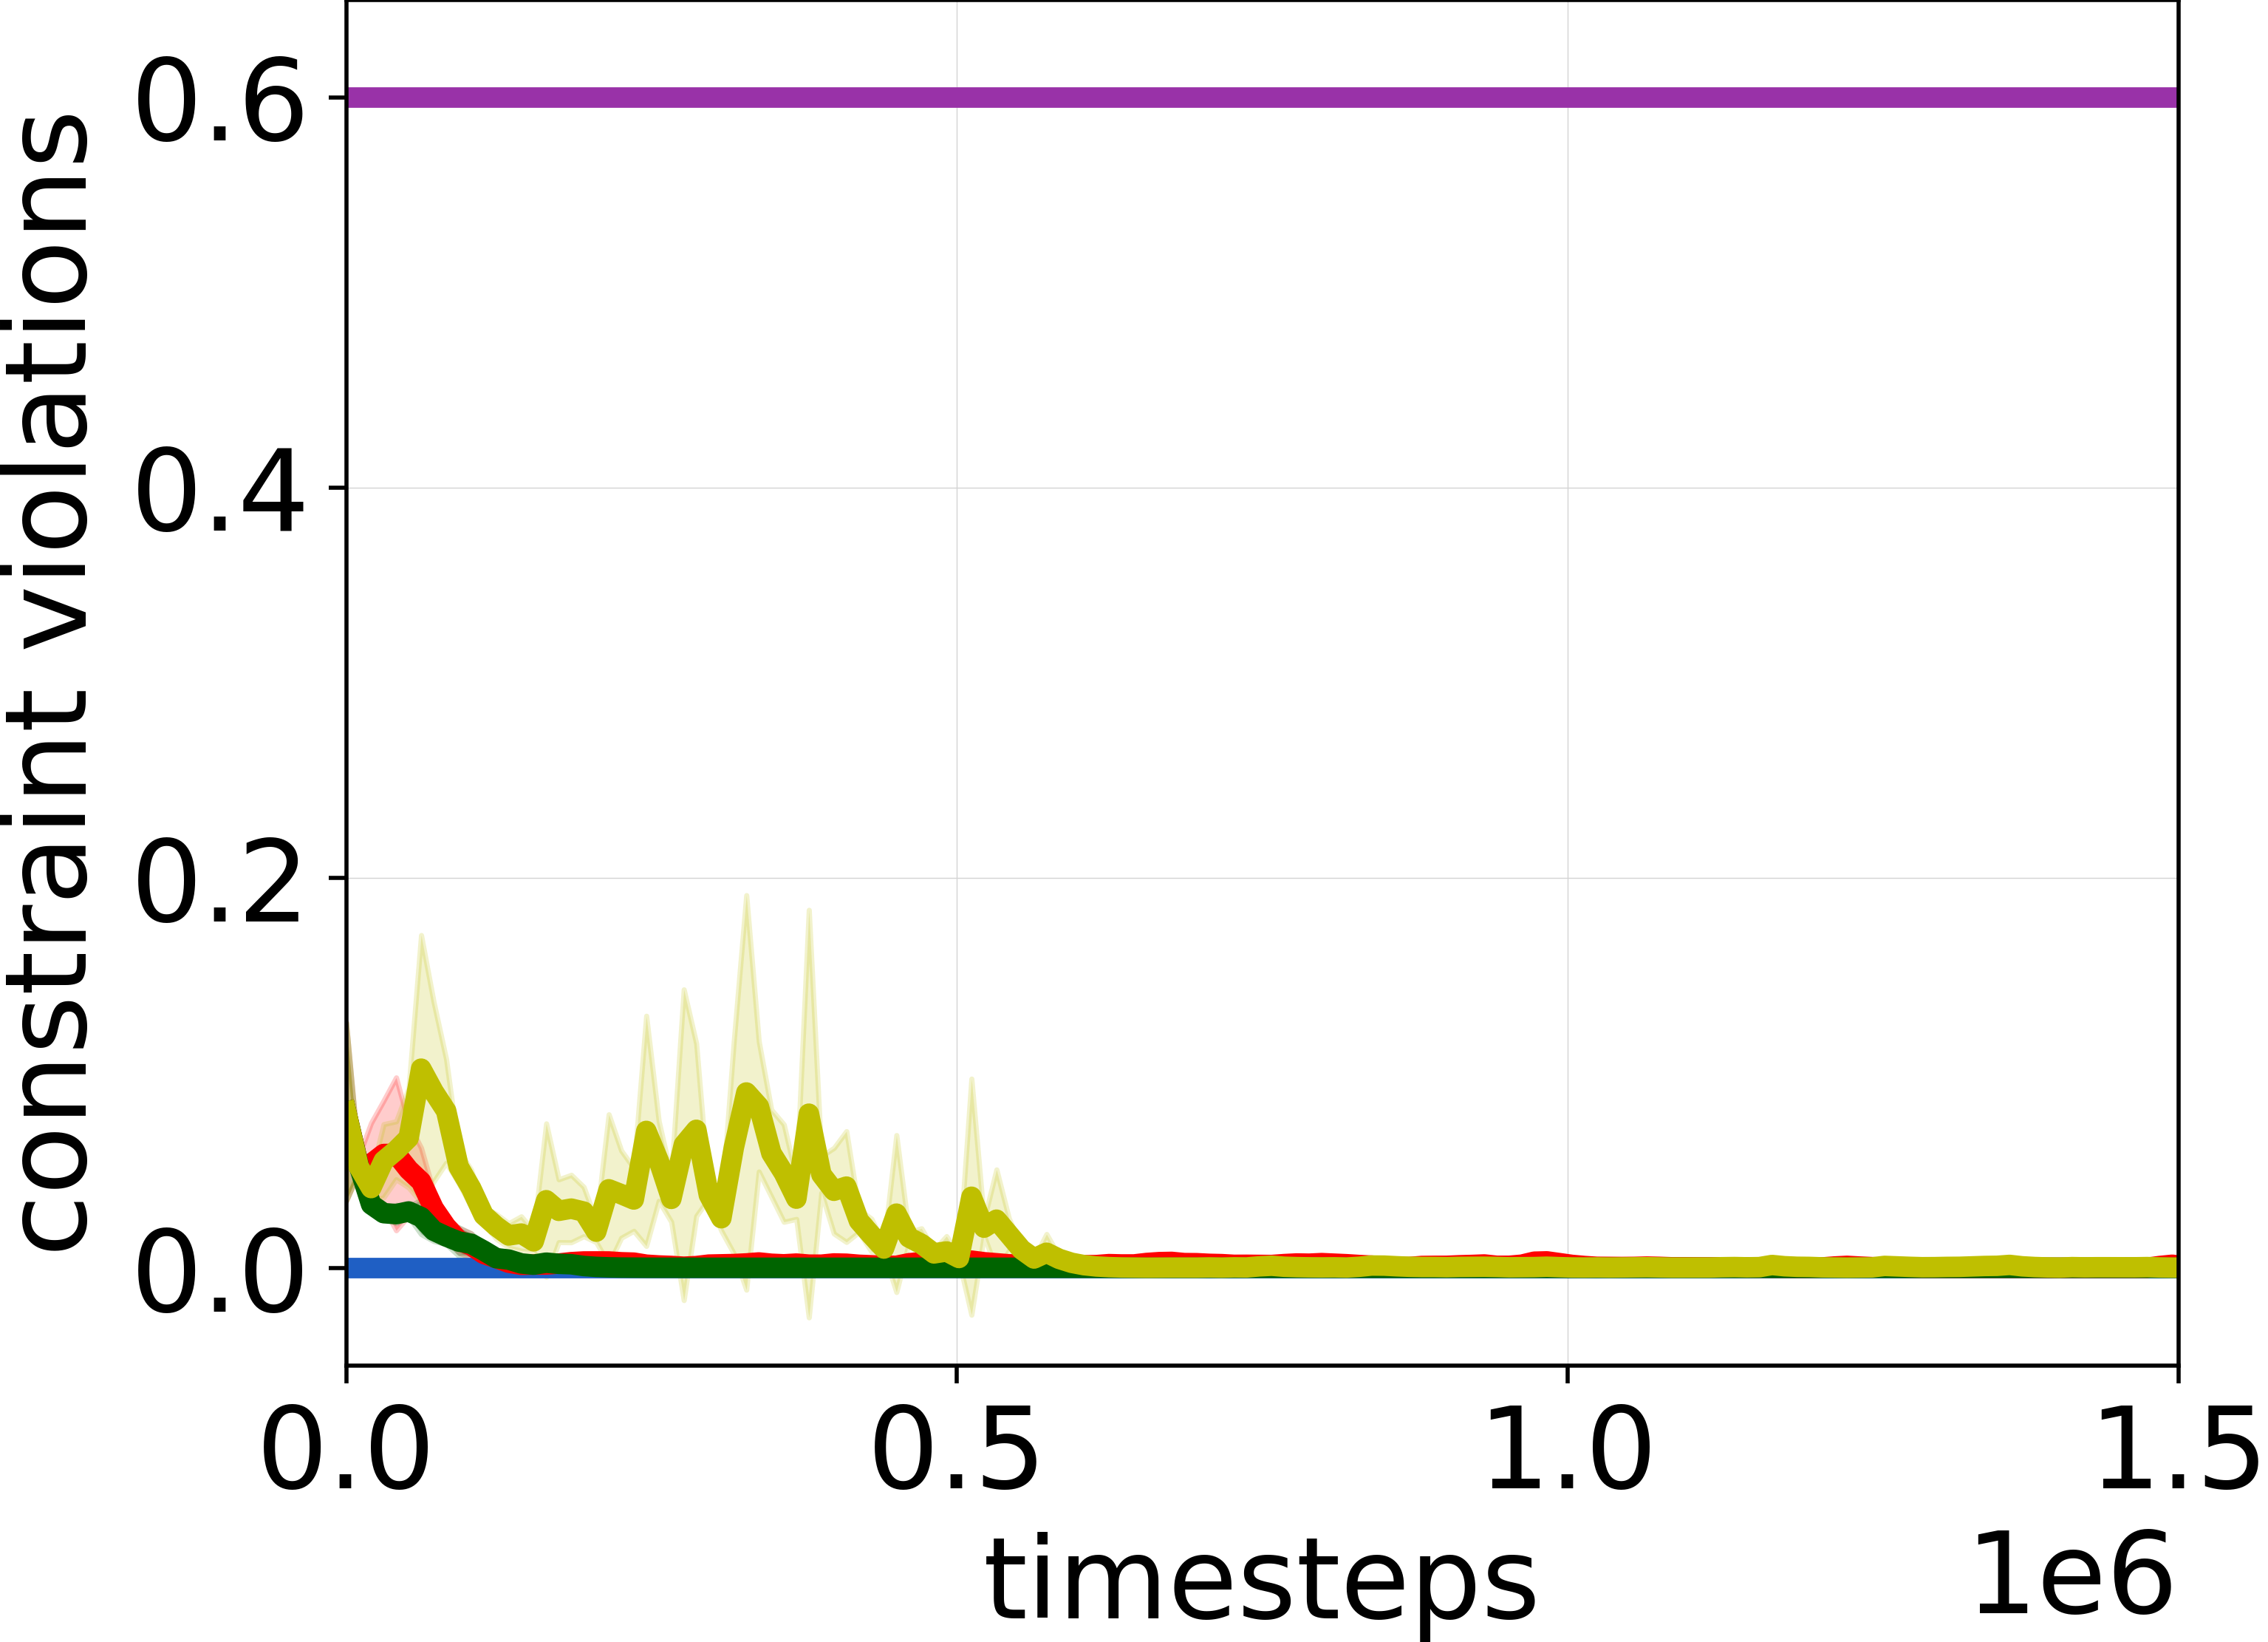
\includegraphics[width=0.20\columnwidth]{figures/point/violations.png}}
    \subfigure[Ant-Broken]{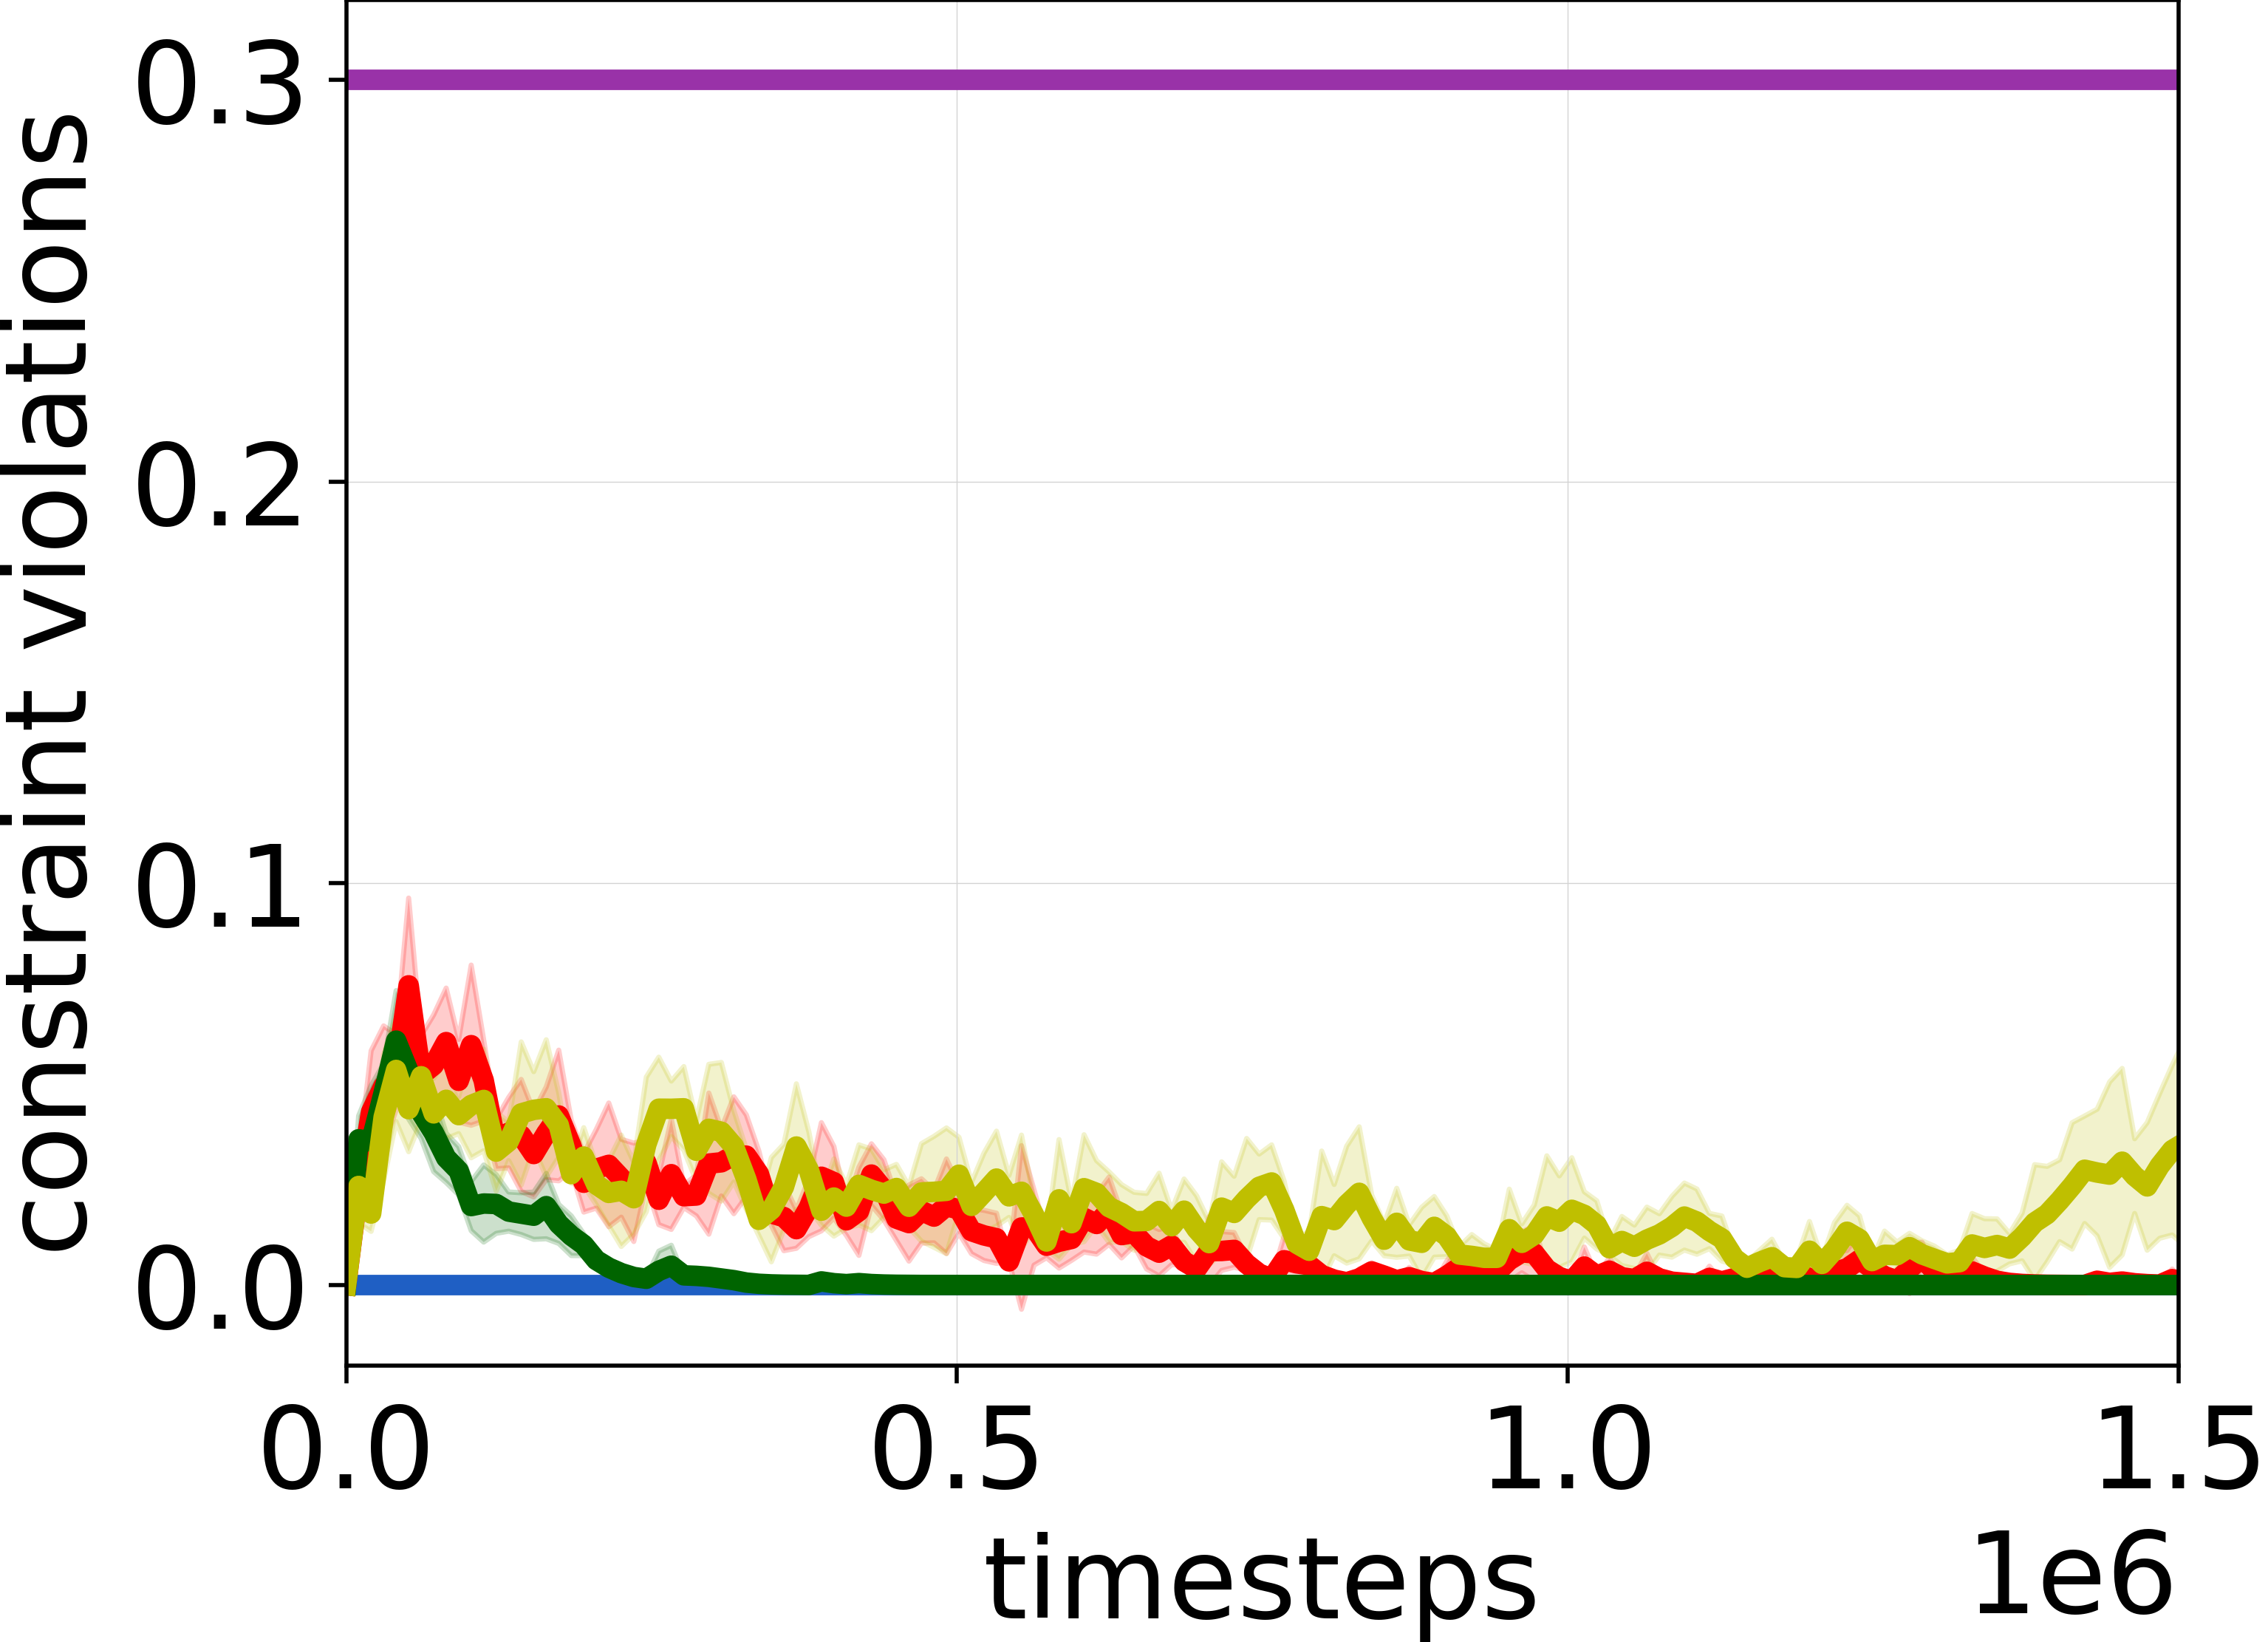
\includegraphics[width=0.20\columnwidth]{figures/ant_broken/violations.png}}\\
    \subfigure{
\includegraphics[width=0.5\columnwidth]{figures/legend.png}}\\
    \caption{\tiny{Transferring constraints. The x-axis is the number of timesteps taken in the environment. All plots were smoothed and averaged over 5 seeds. The shaded regions correspond to the standard error.}}
    \label{fig:transfer}
\end{center}
\end{figure}
\end{frame}


\begin{frame}{Ablation Studies}
\begin{figure}
\begin{center}
    \small{\bfseries Reward (higher is better):}\\
    \subfigure{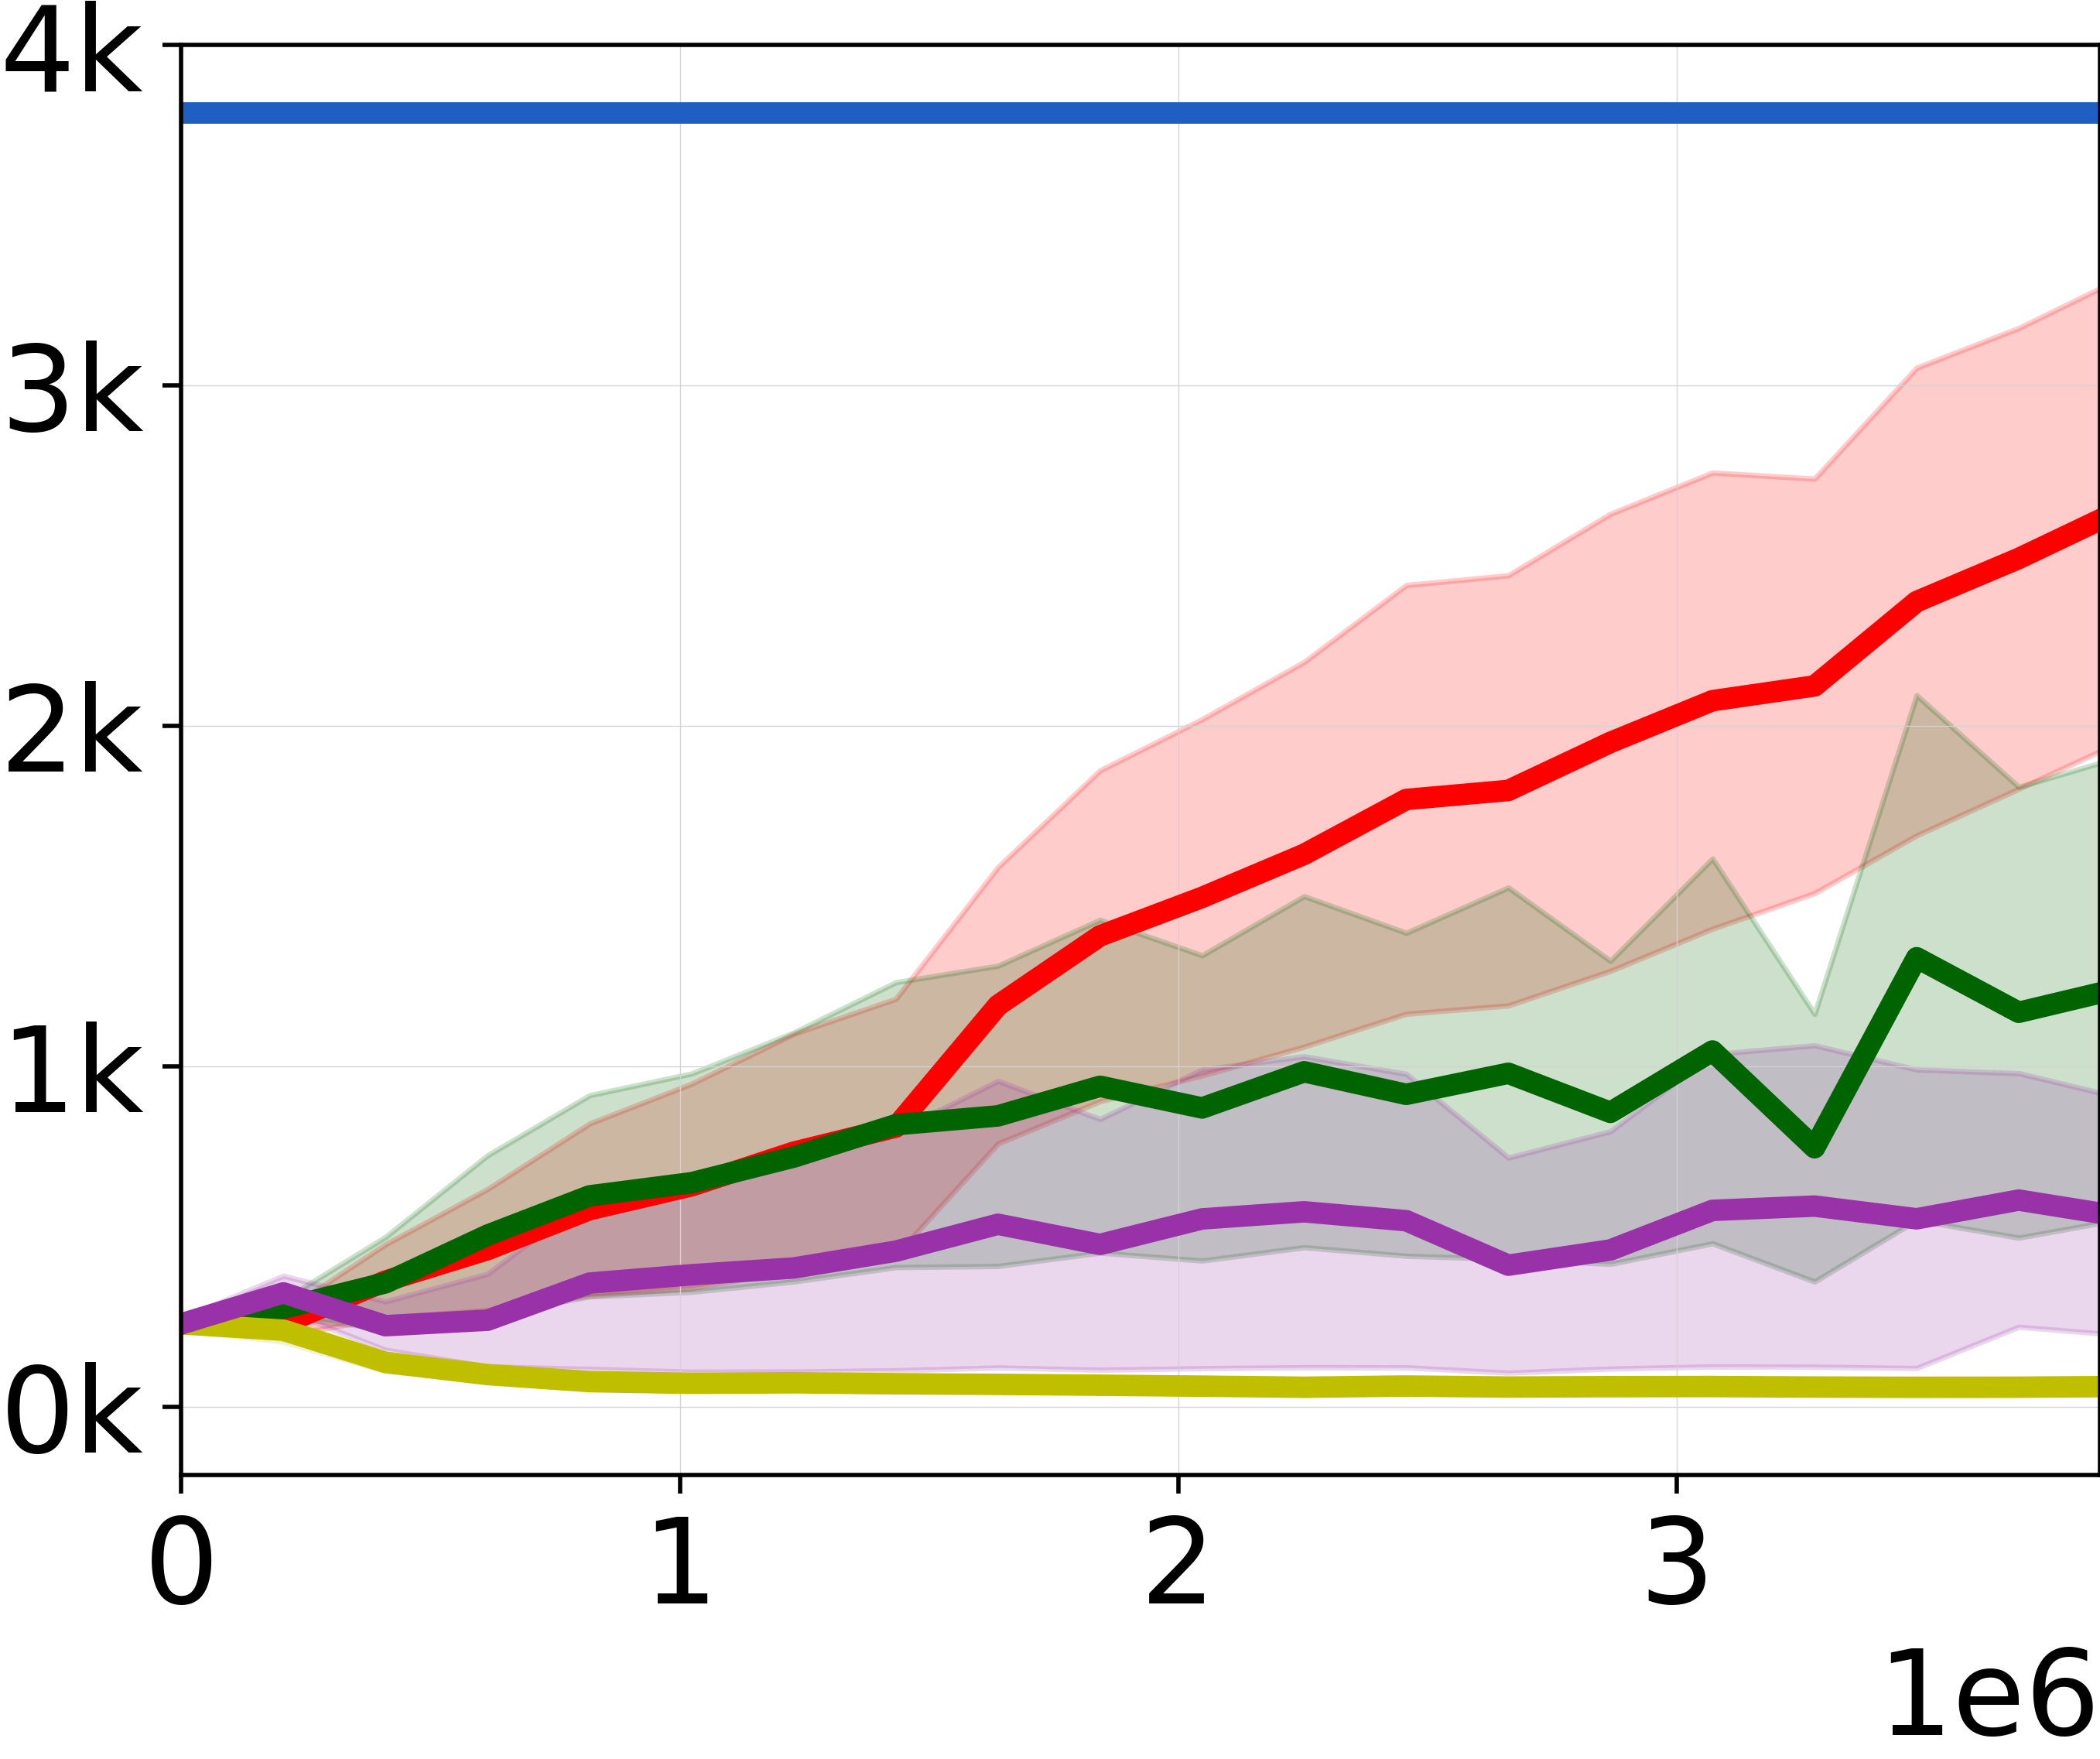
\includegraphics[width=0.18\textwidth]{figures/ablations/no-is_no-es/reward.png}}
    \subfigure{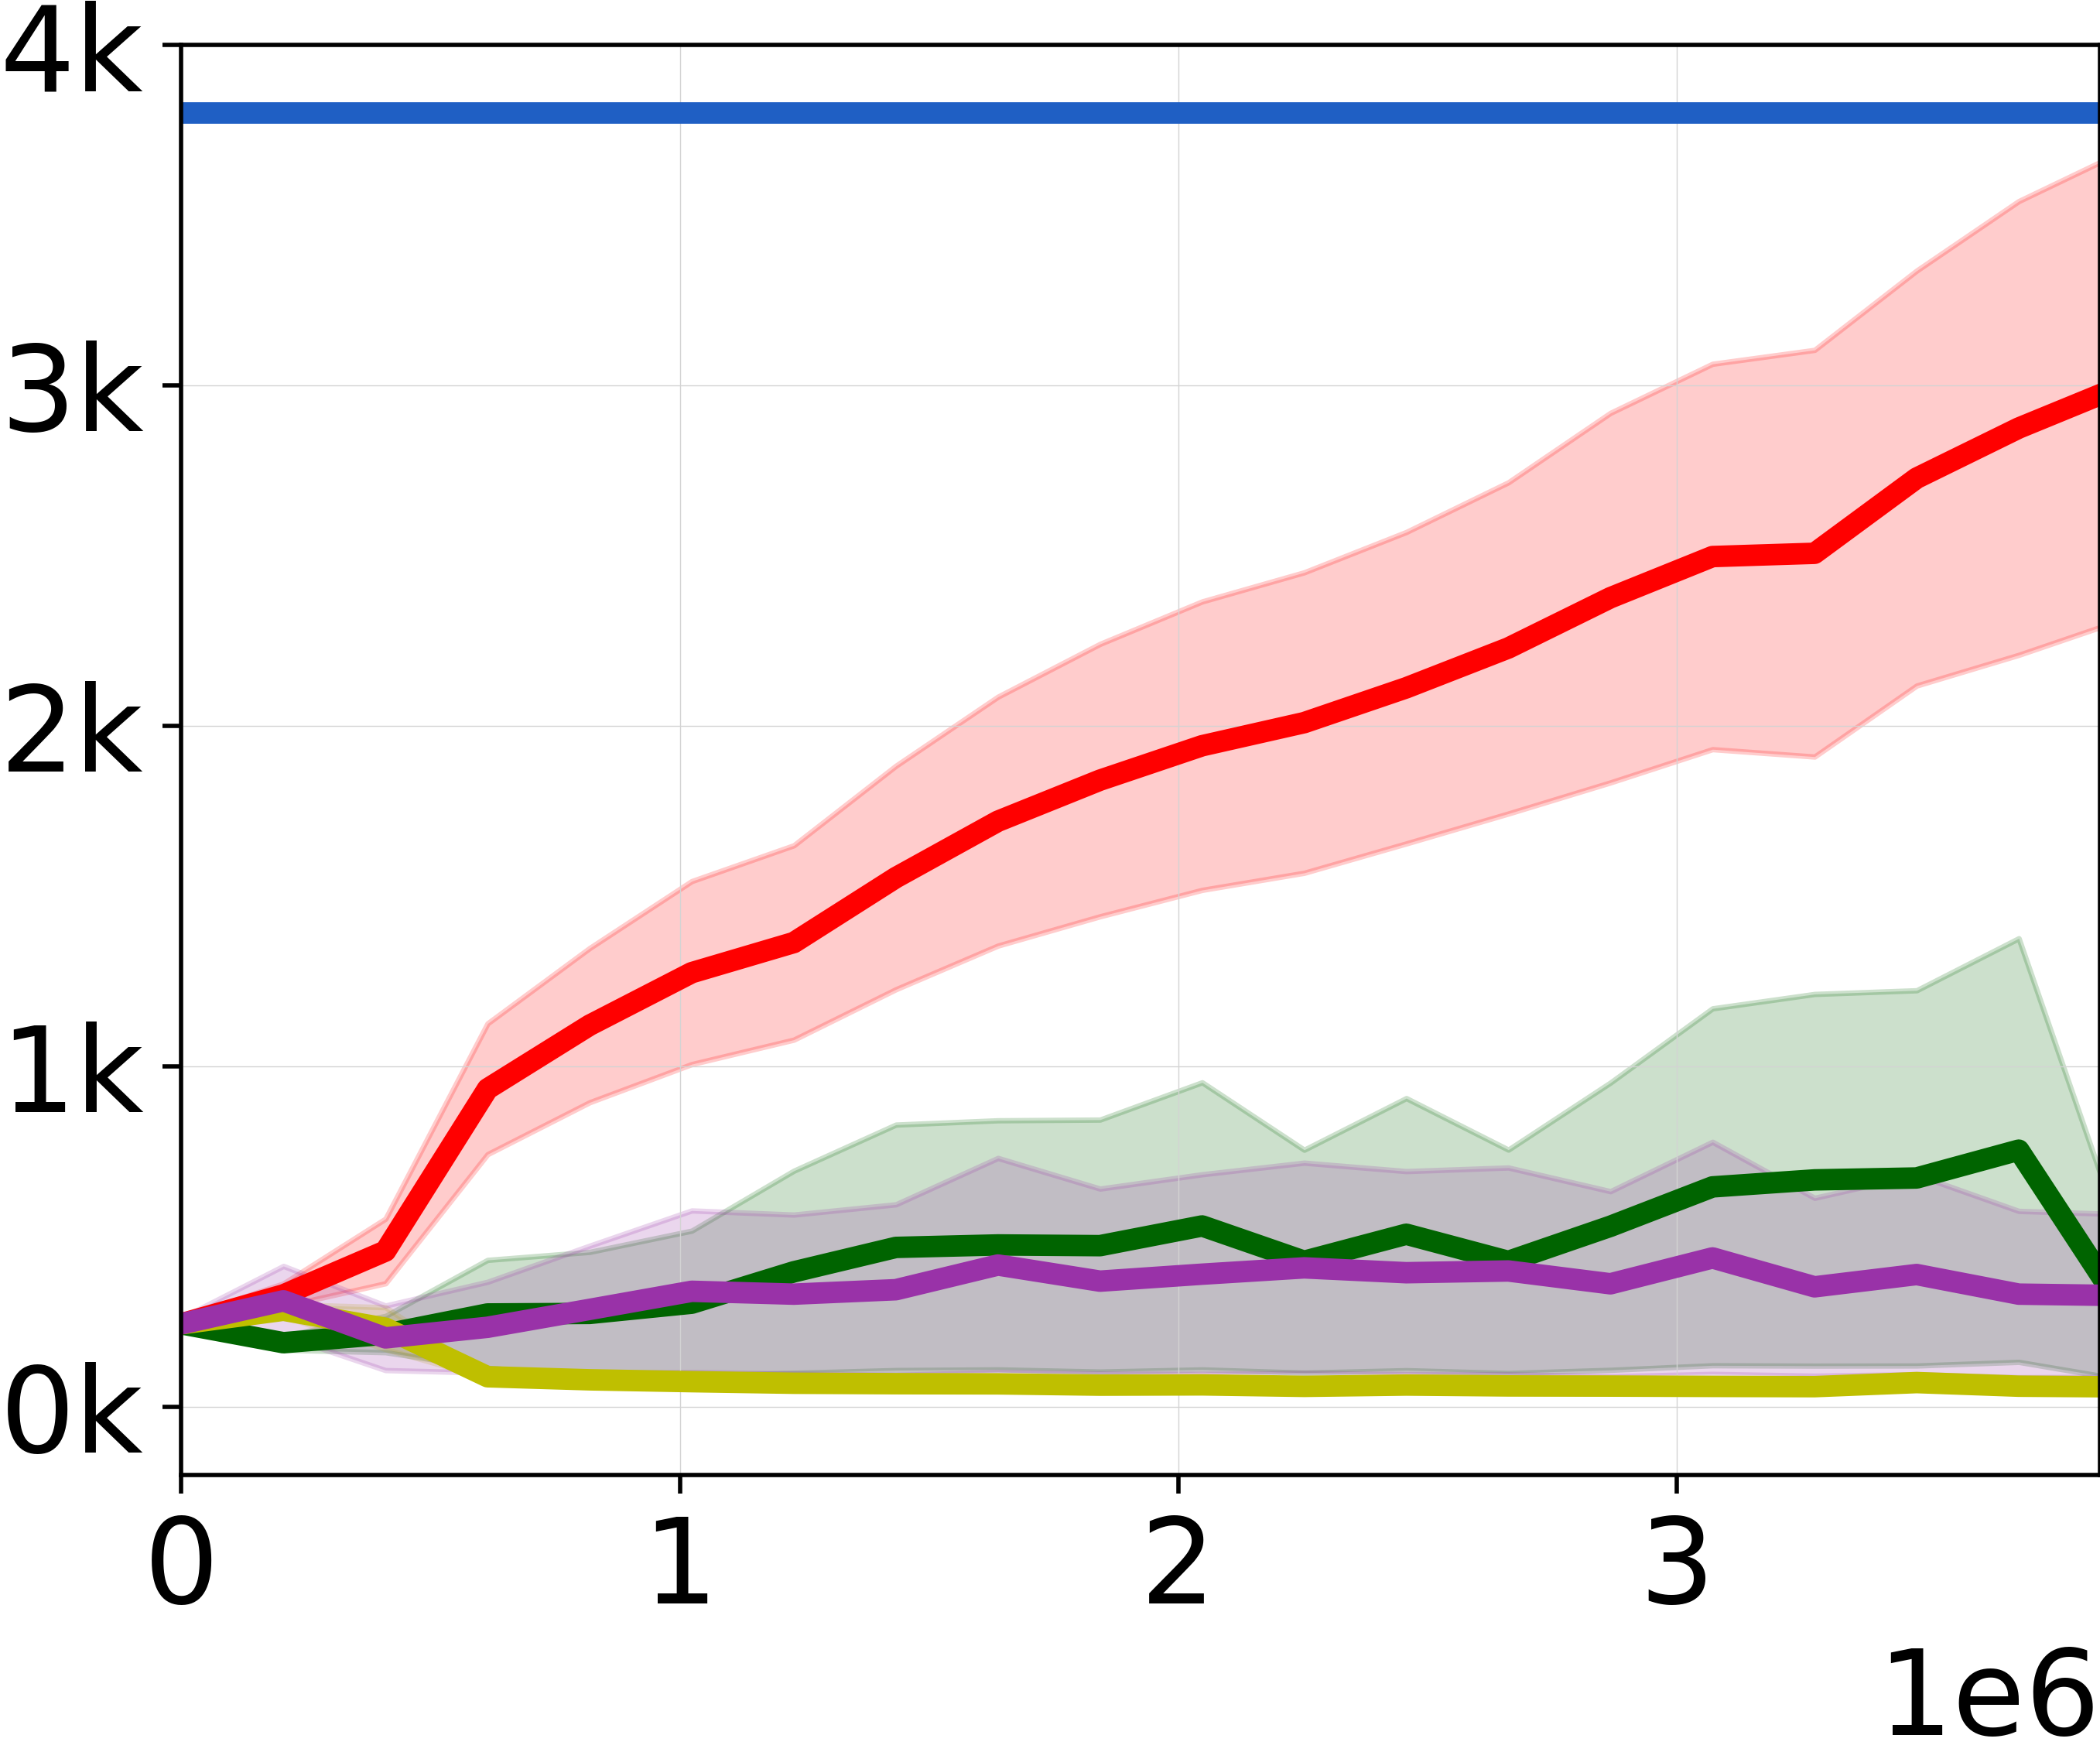
\includegraphics[width=0.18\textwidth]{figures/ablations/no-is_es/reward.png}}
    \subfigure{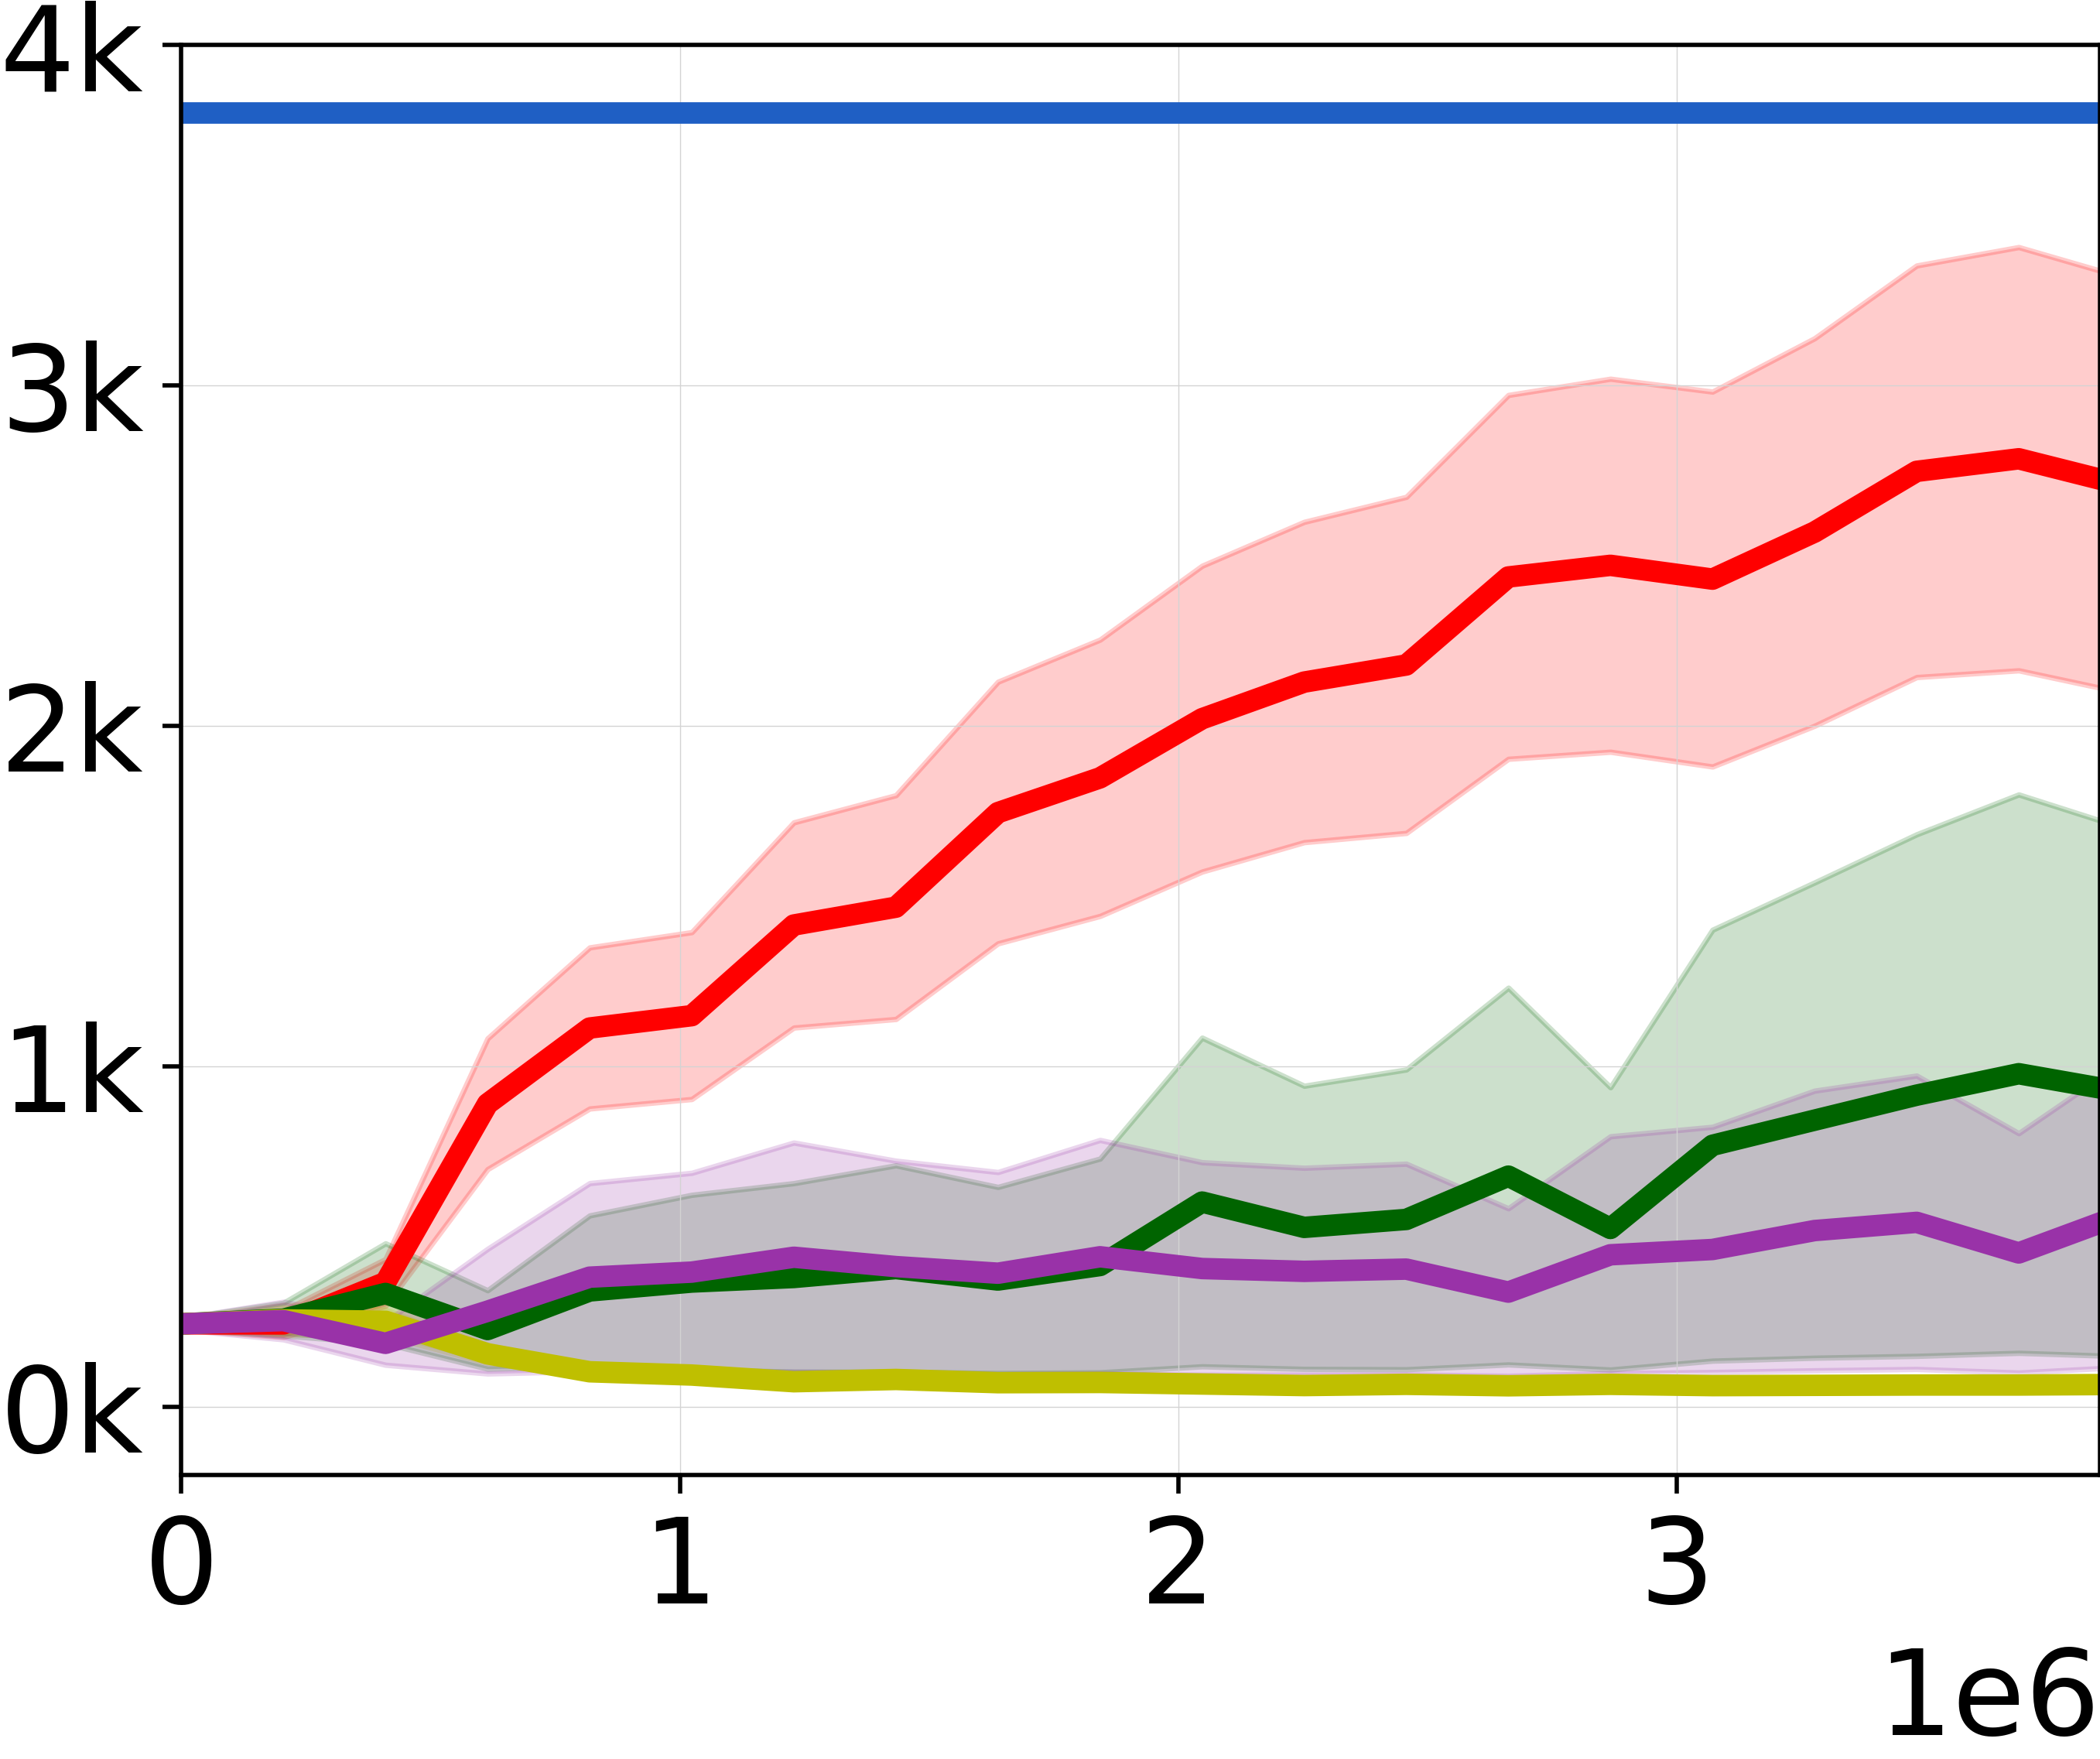
\includegraphics[width=0.18\textwidth]{figures/ablations/is_no-es/reward.png}}
    \subfigure{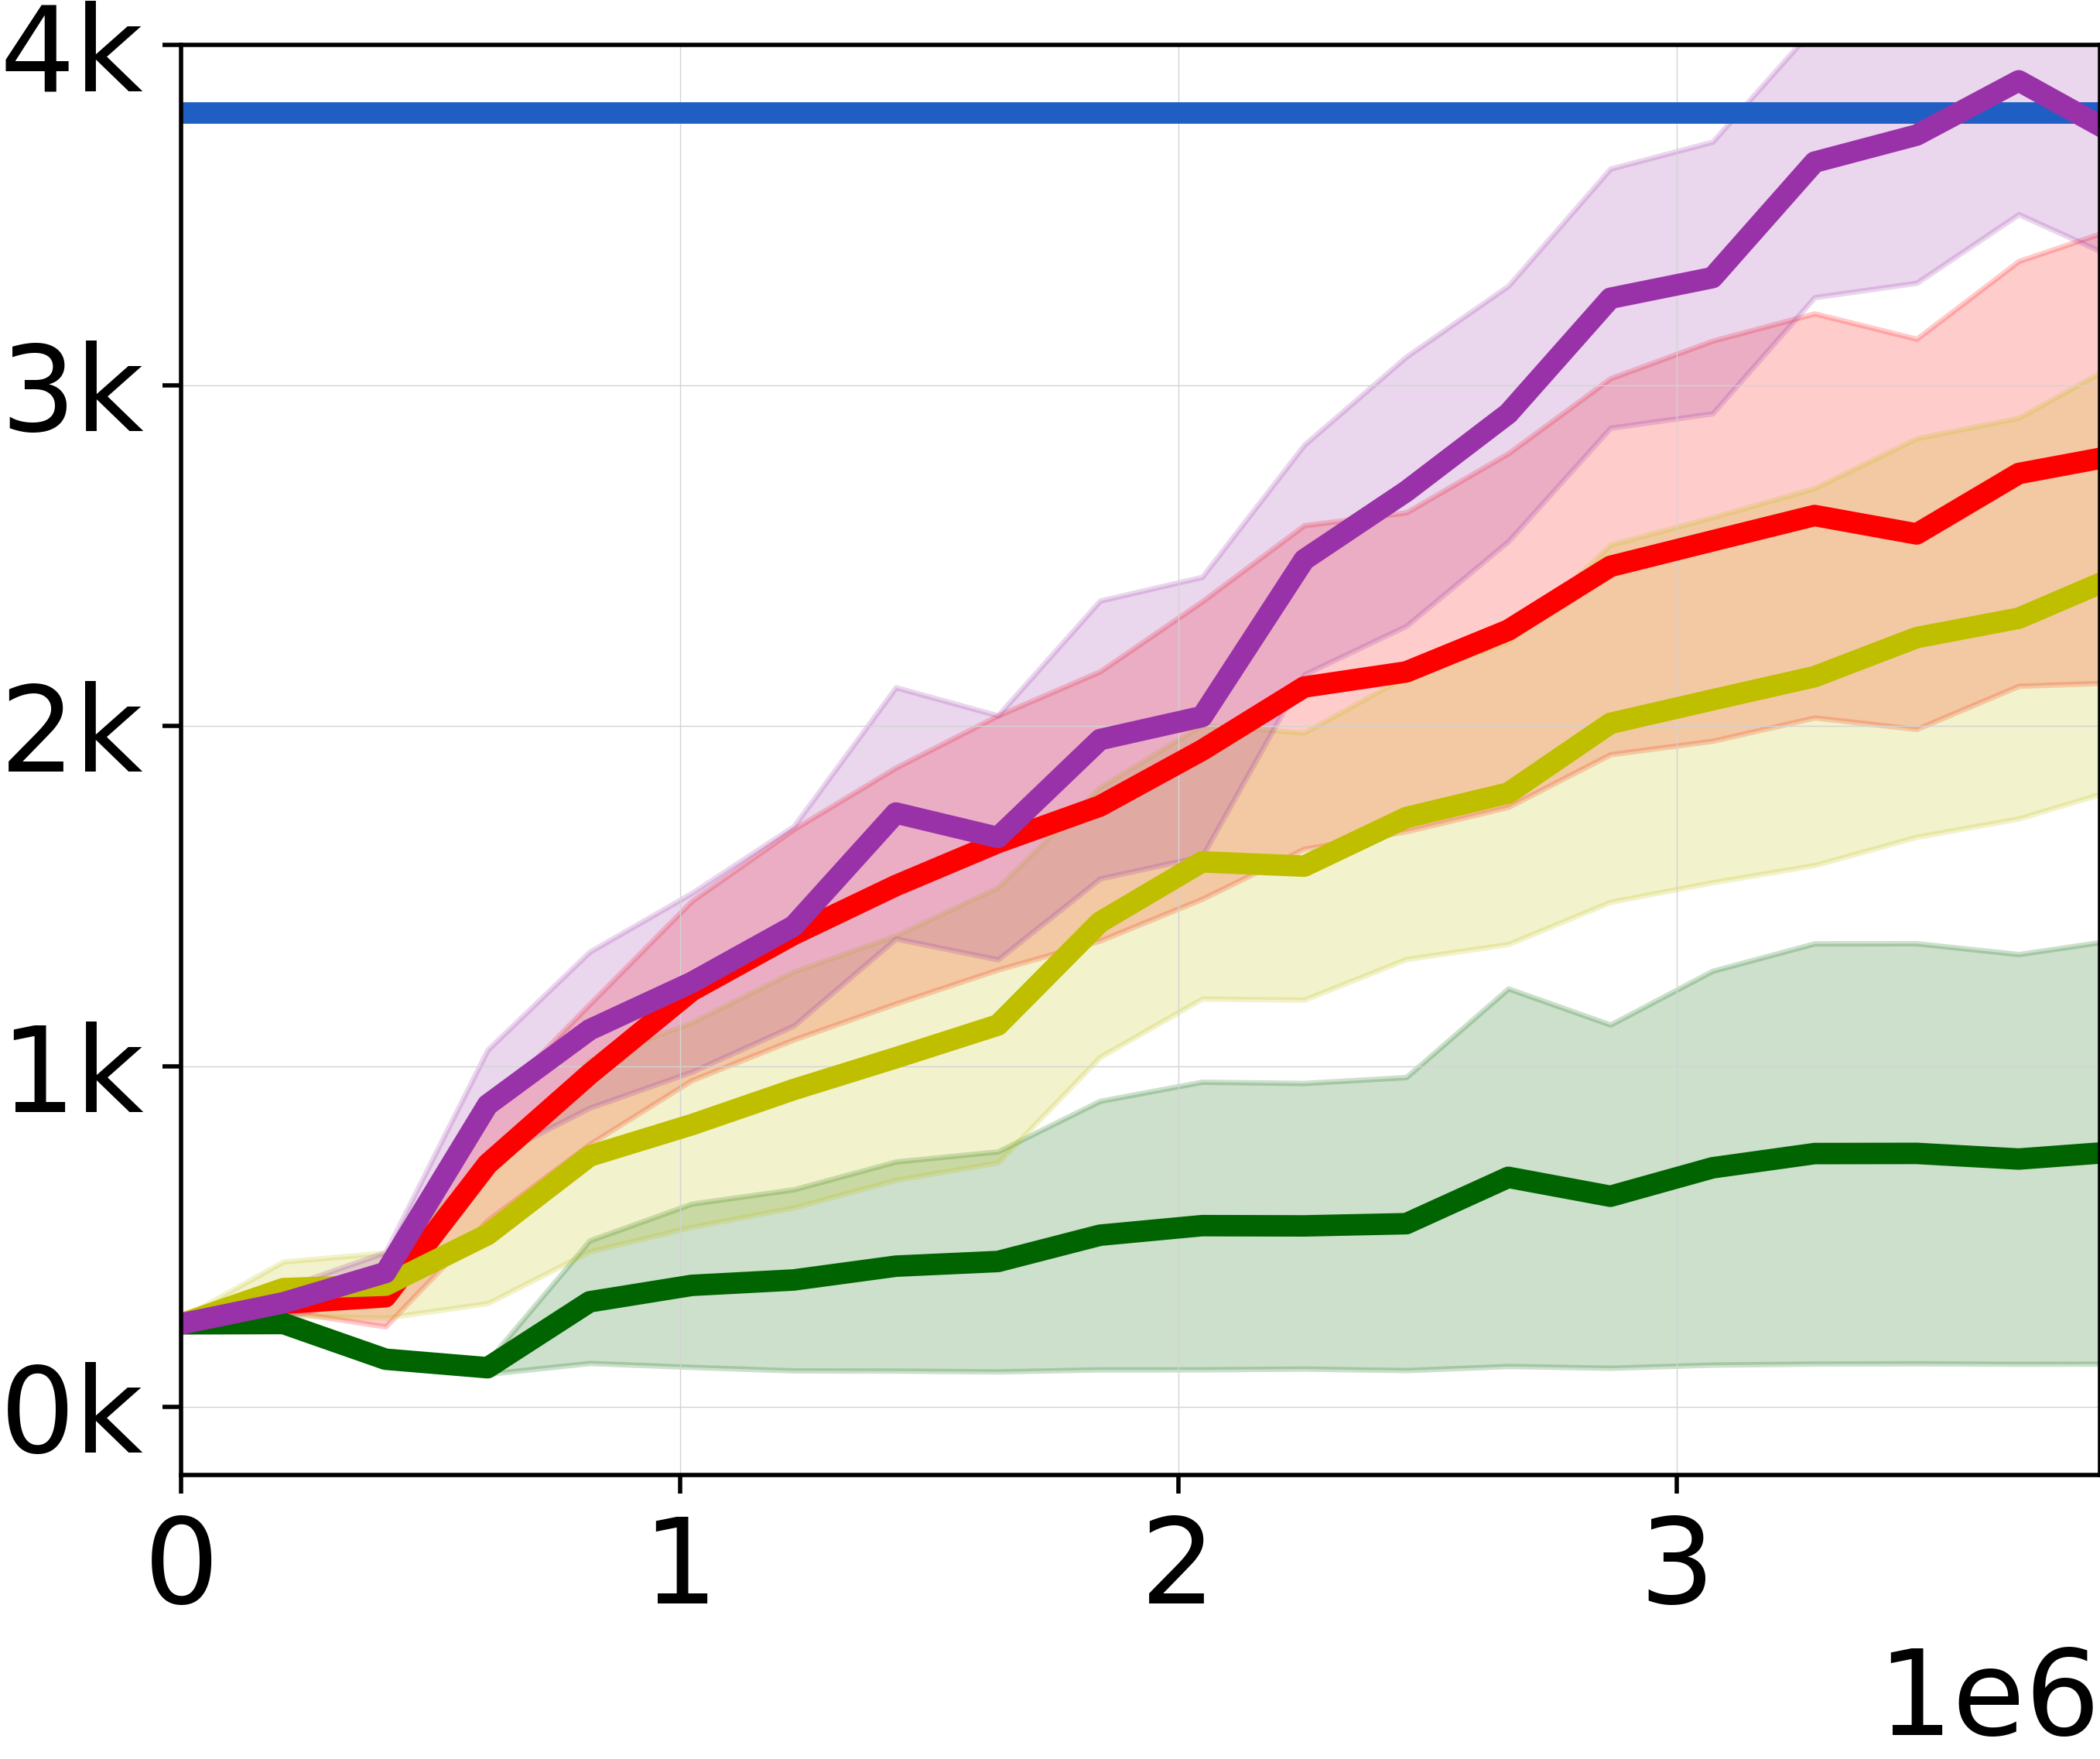
\includegraphics[width=0.18\textwidth]{figures/ablations/is_es/reward.png}}\\
    \setcounter{subfigure}{0}
    \small{\bfseries Constraint violations (lower is better):}\\
    \subfigure[No IS and no ES]{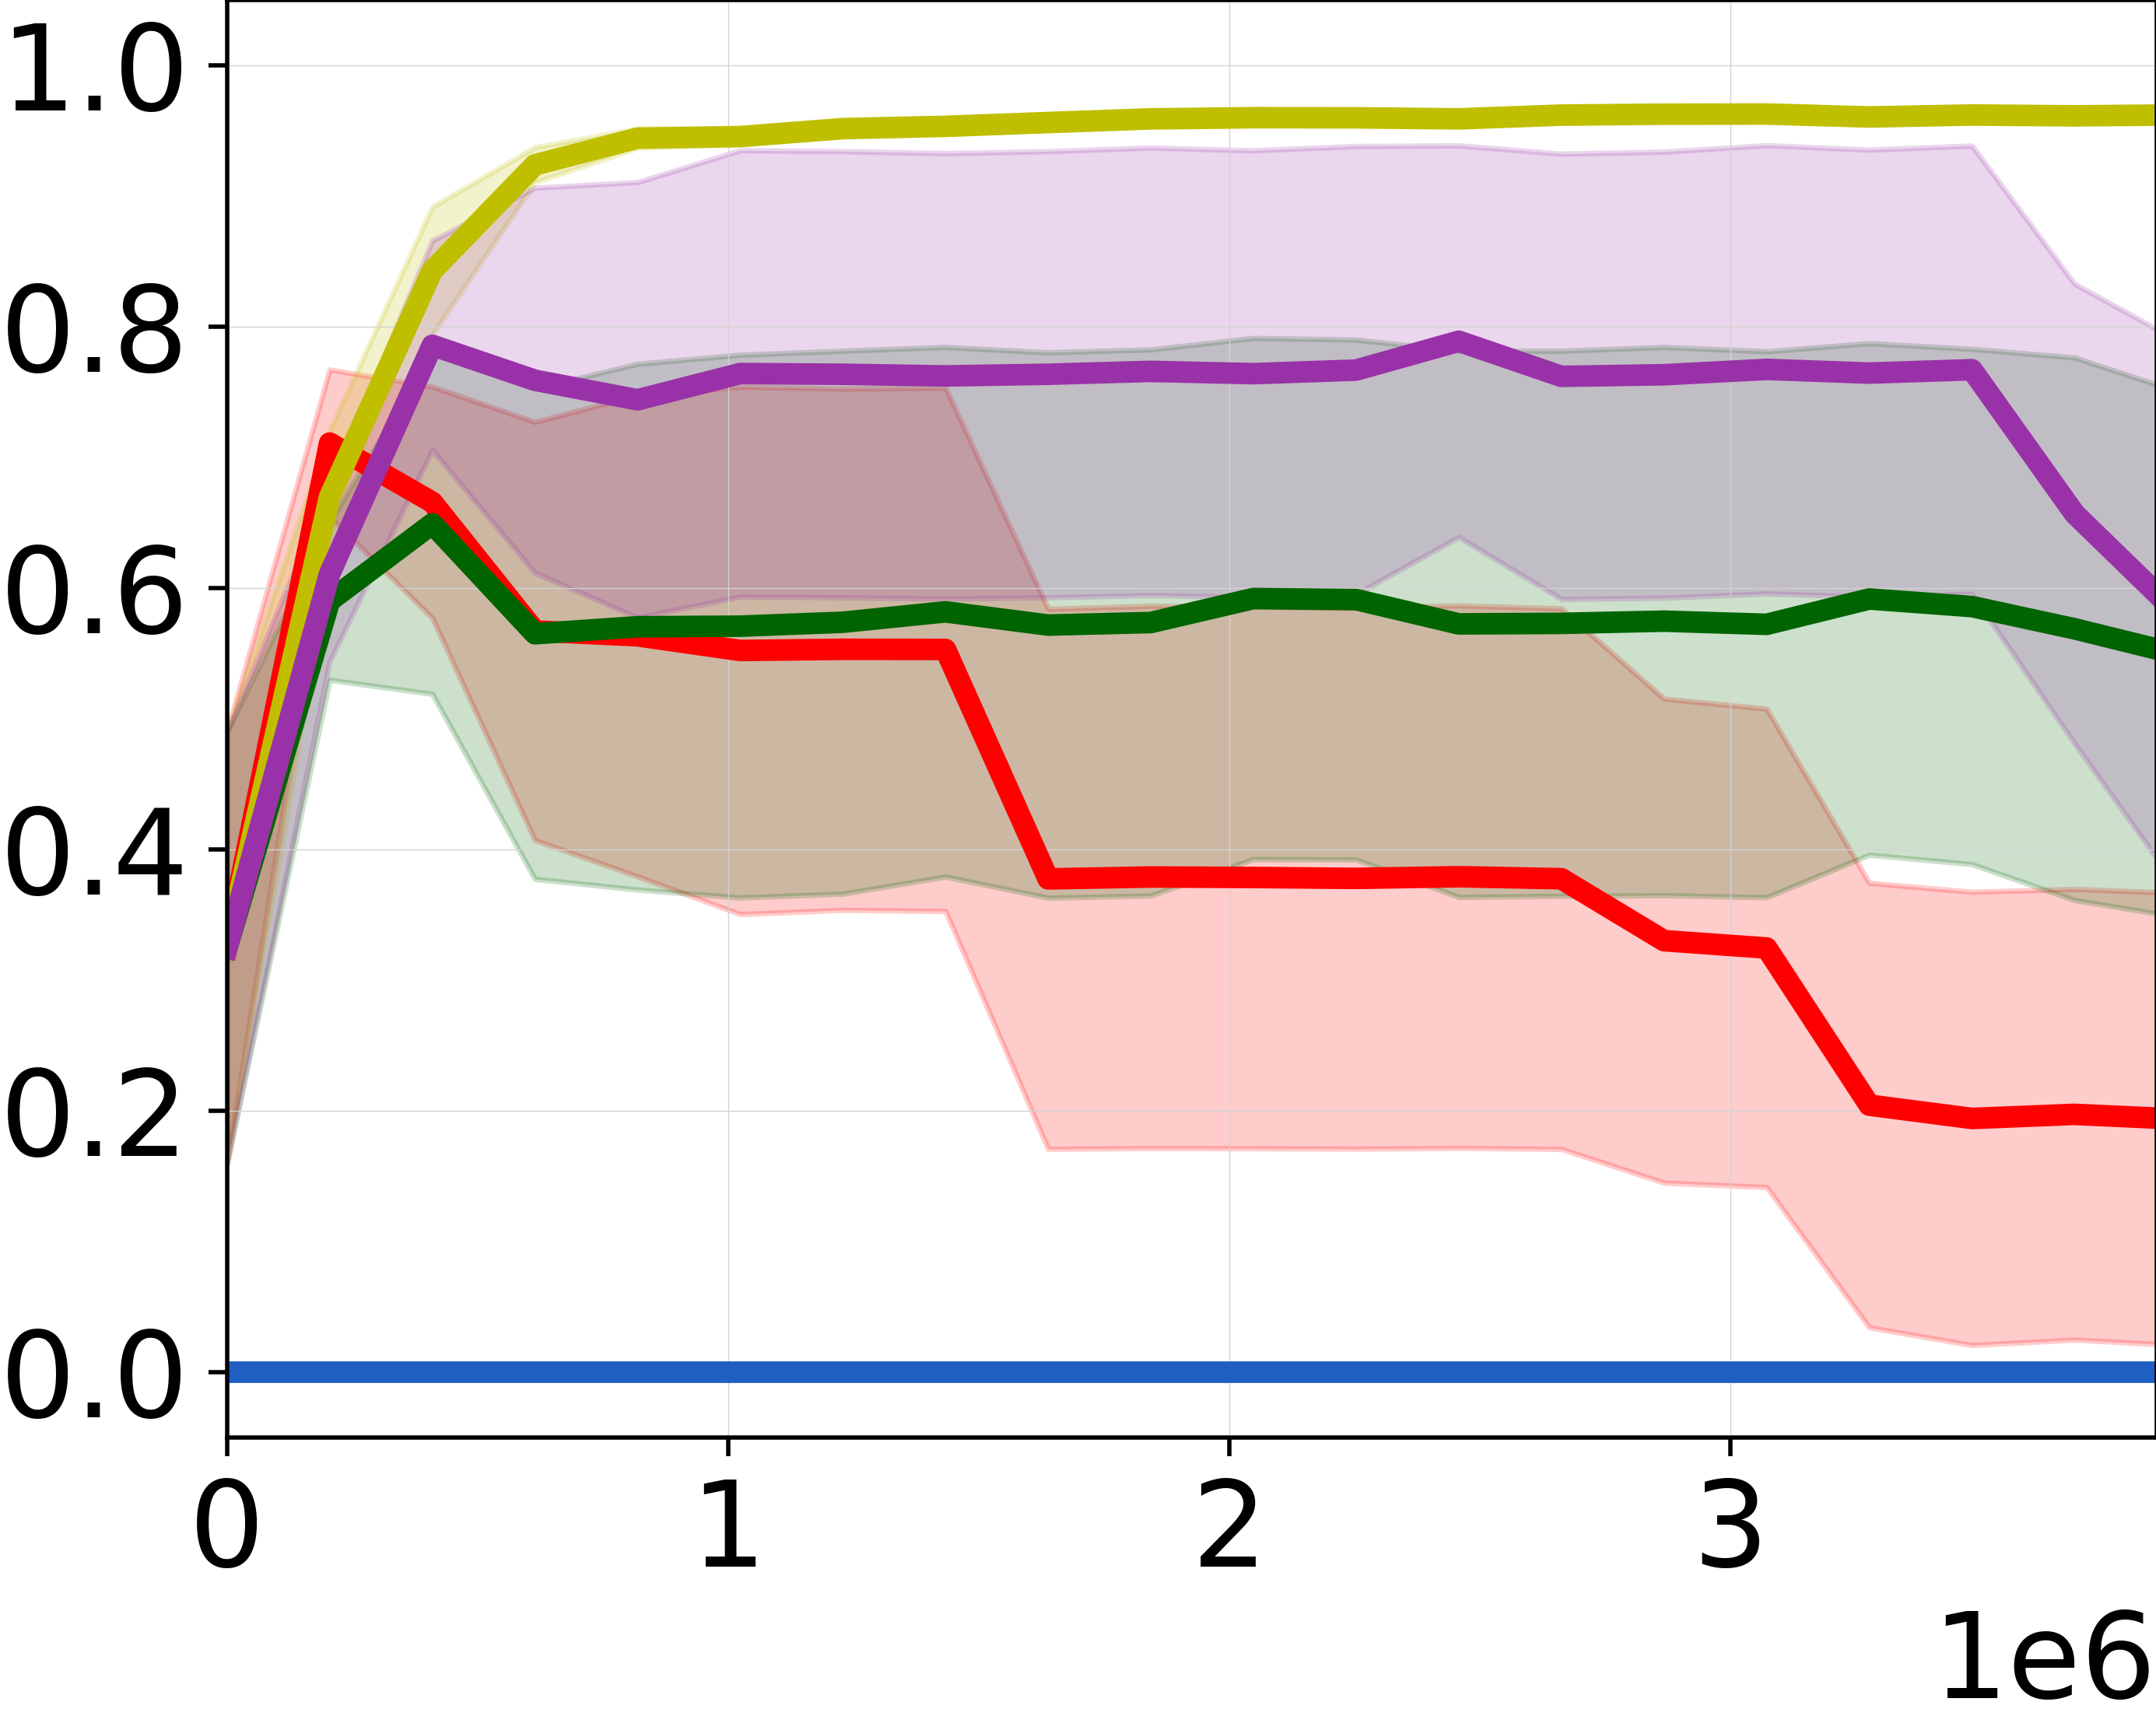
\includegraphics[width=0.18\textwidth]{figures/ablations/no-is_no-es/violations.png}}
    \subfigure[No IS but ES]{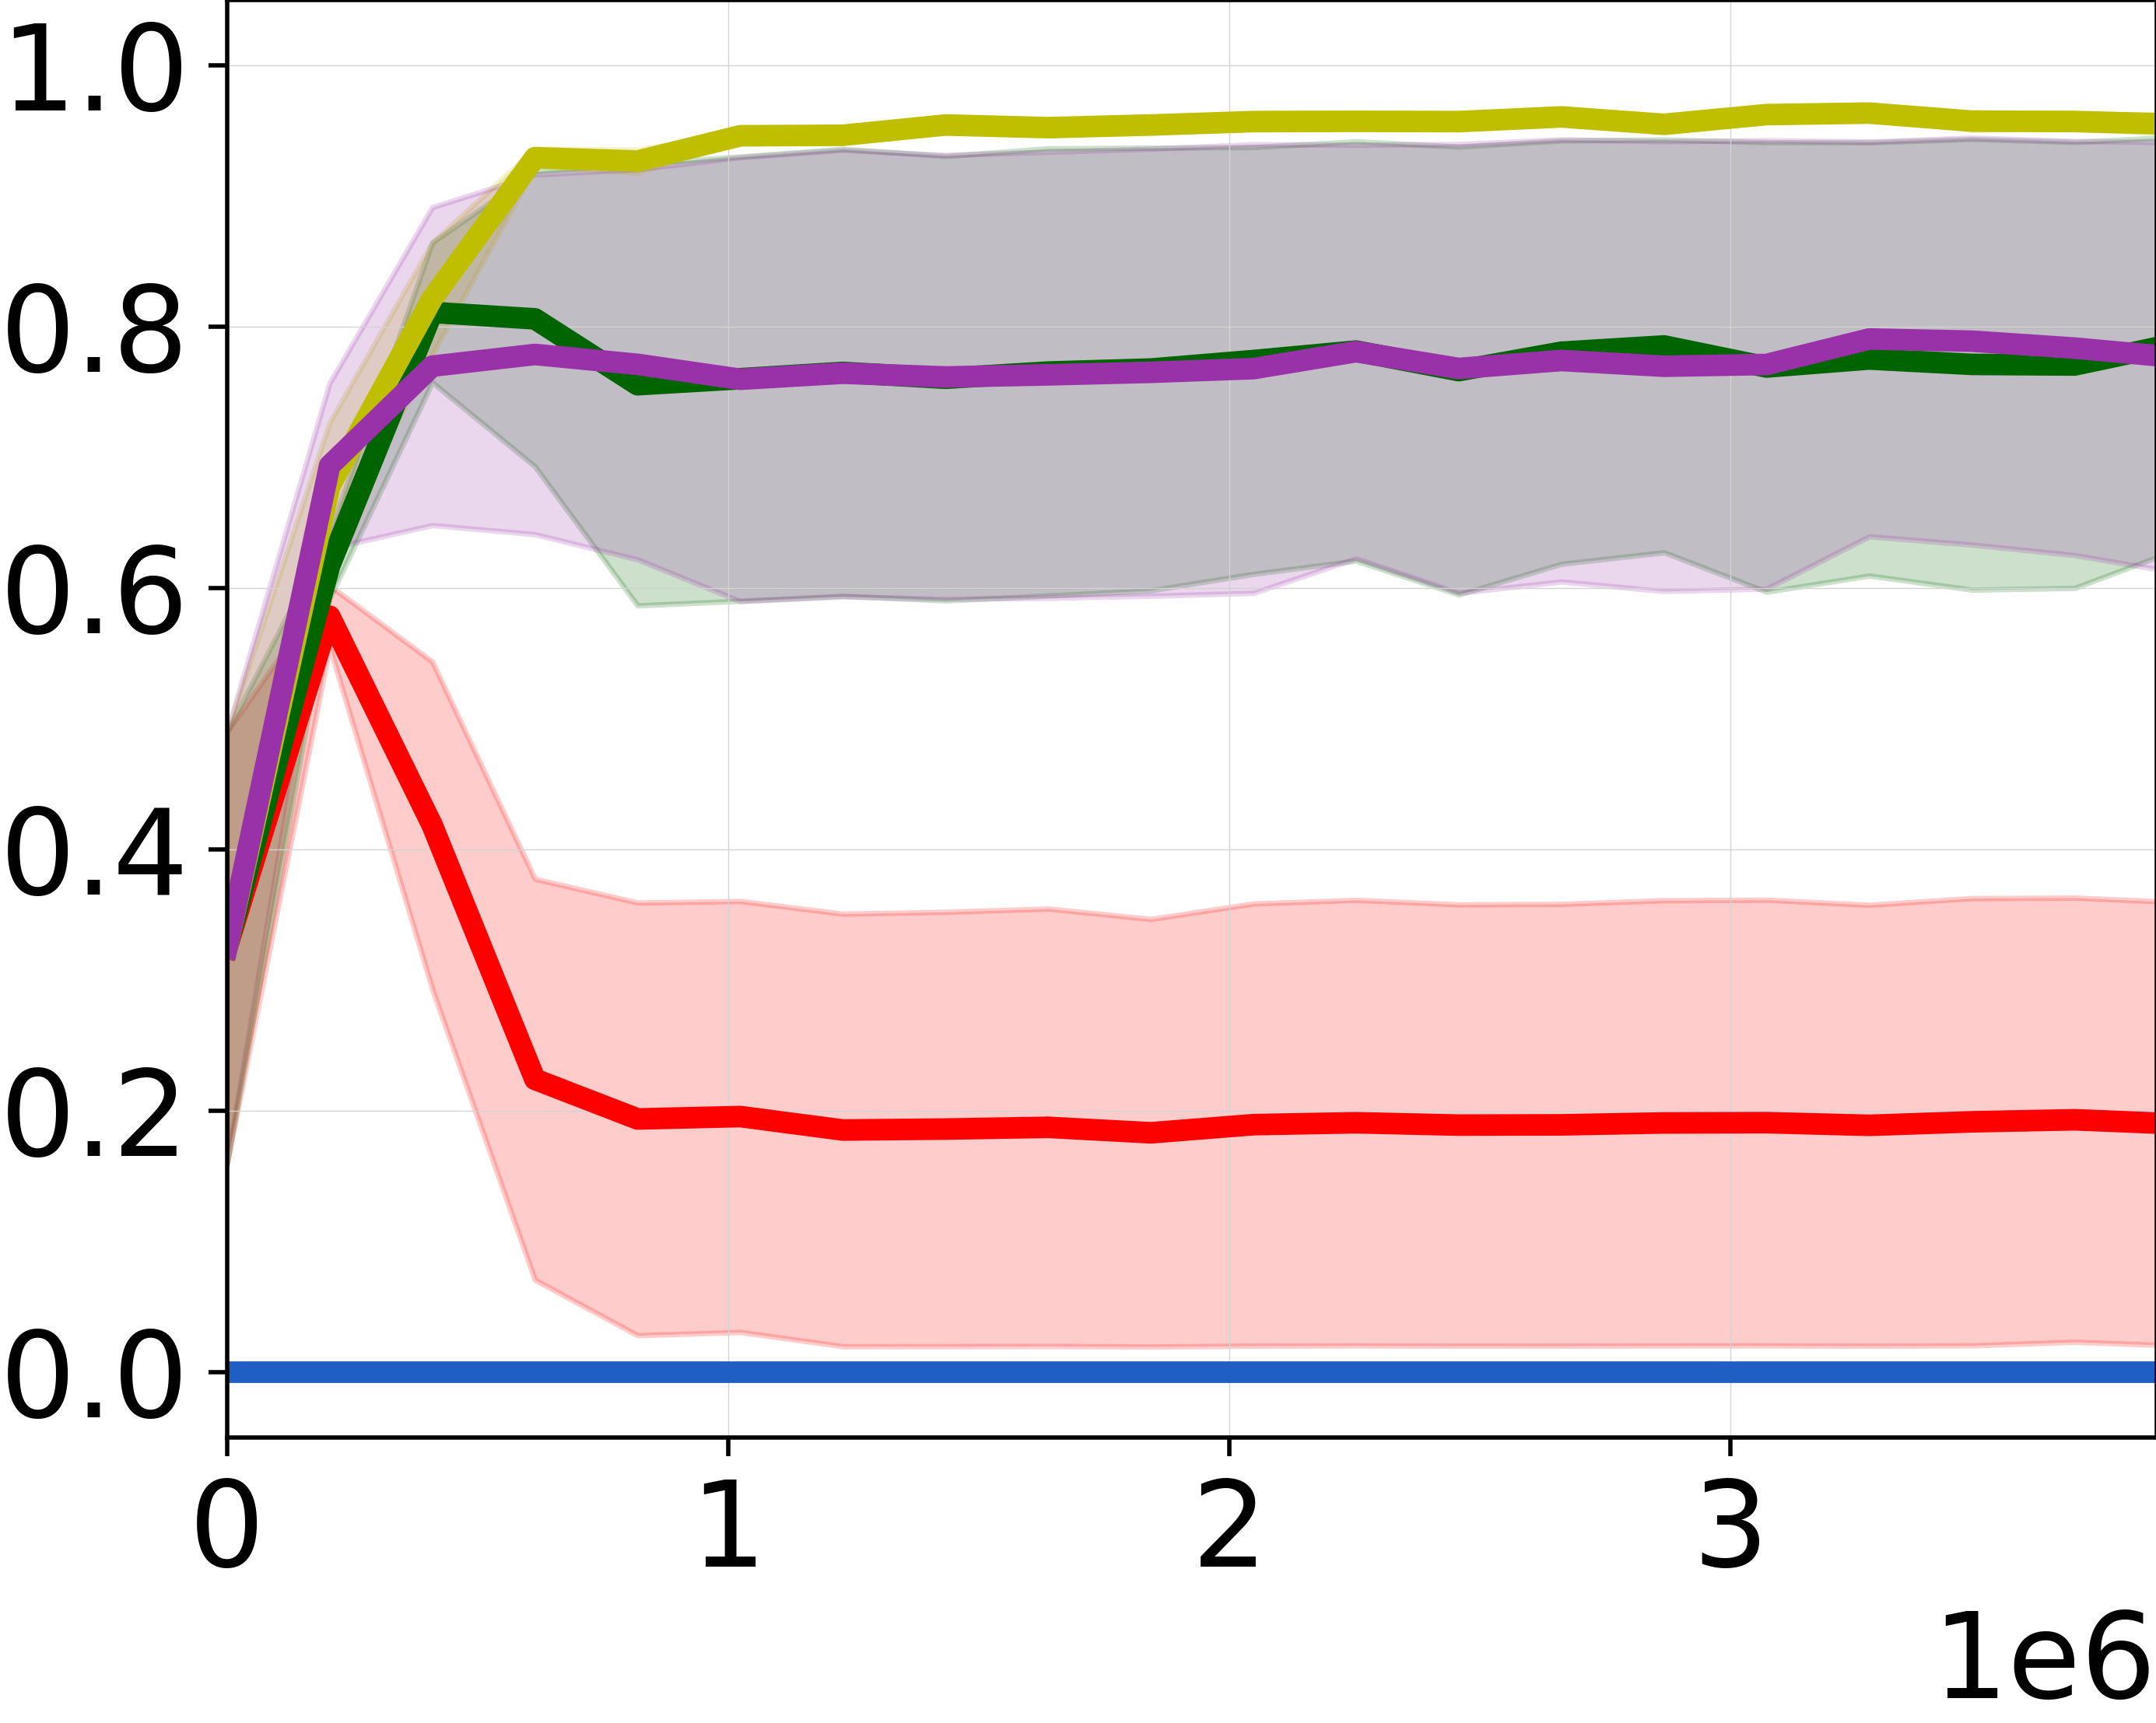
\includegraphics[width=0.18\textwidth]{figures/ablations/no-is_es/violations.png}}
    \subfigure[IS but no ES]{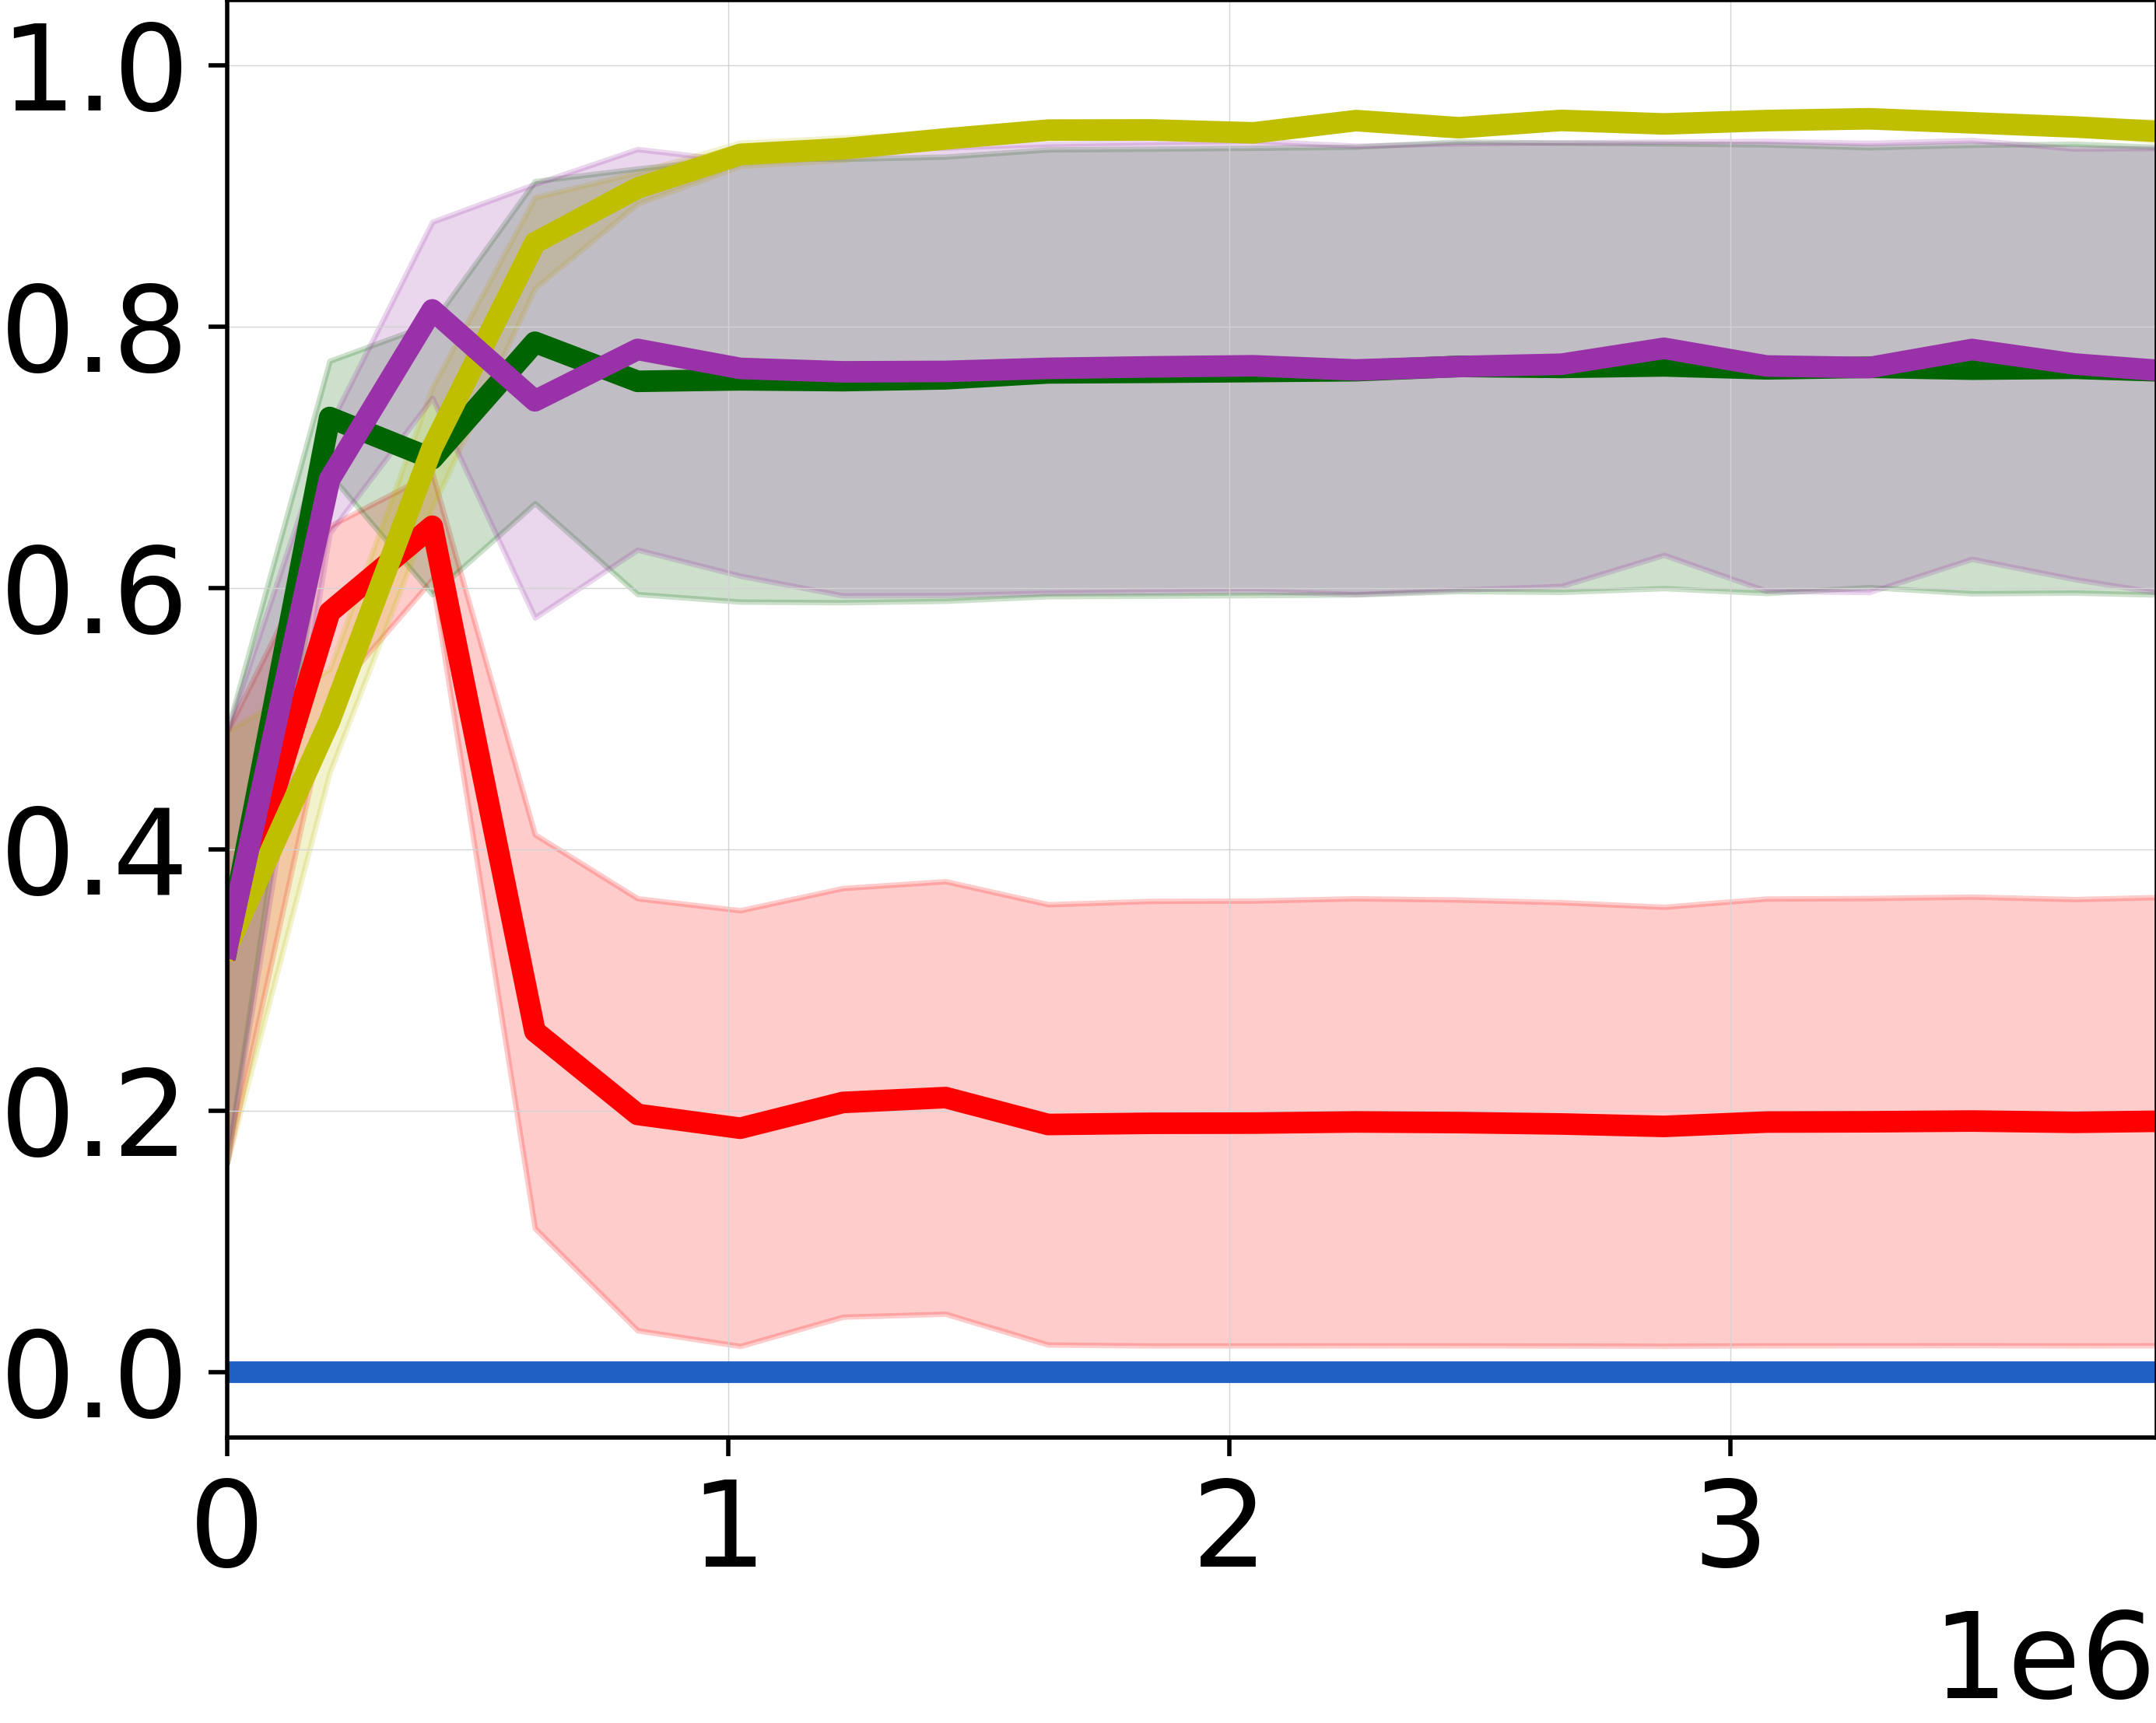
\includegraphics[width=0.18\textwidth]{figures/ablations/is_no-es/violations.png}}
    \subfigure[IS and ES]{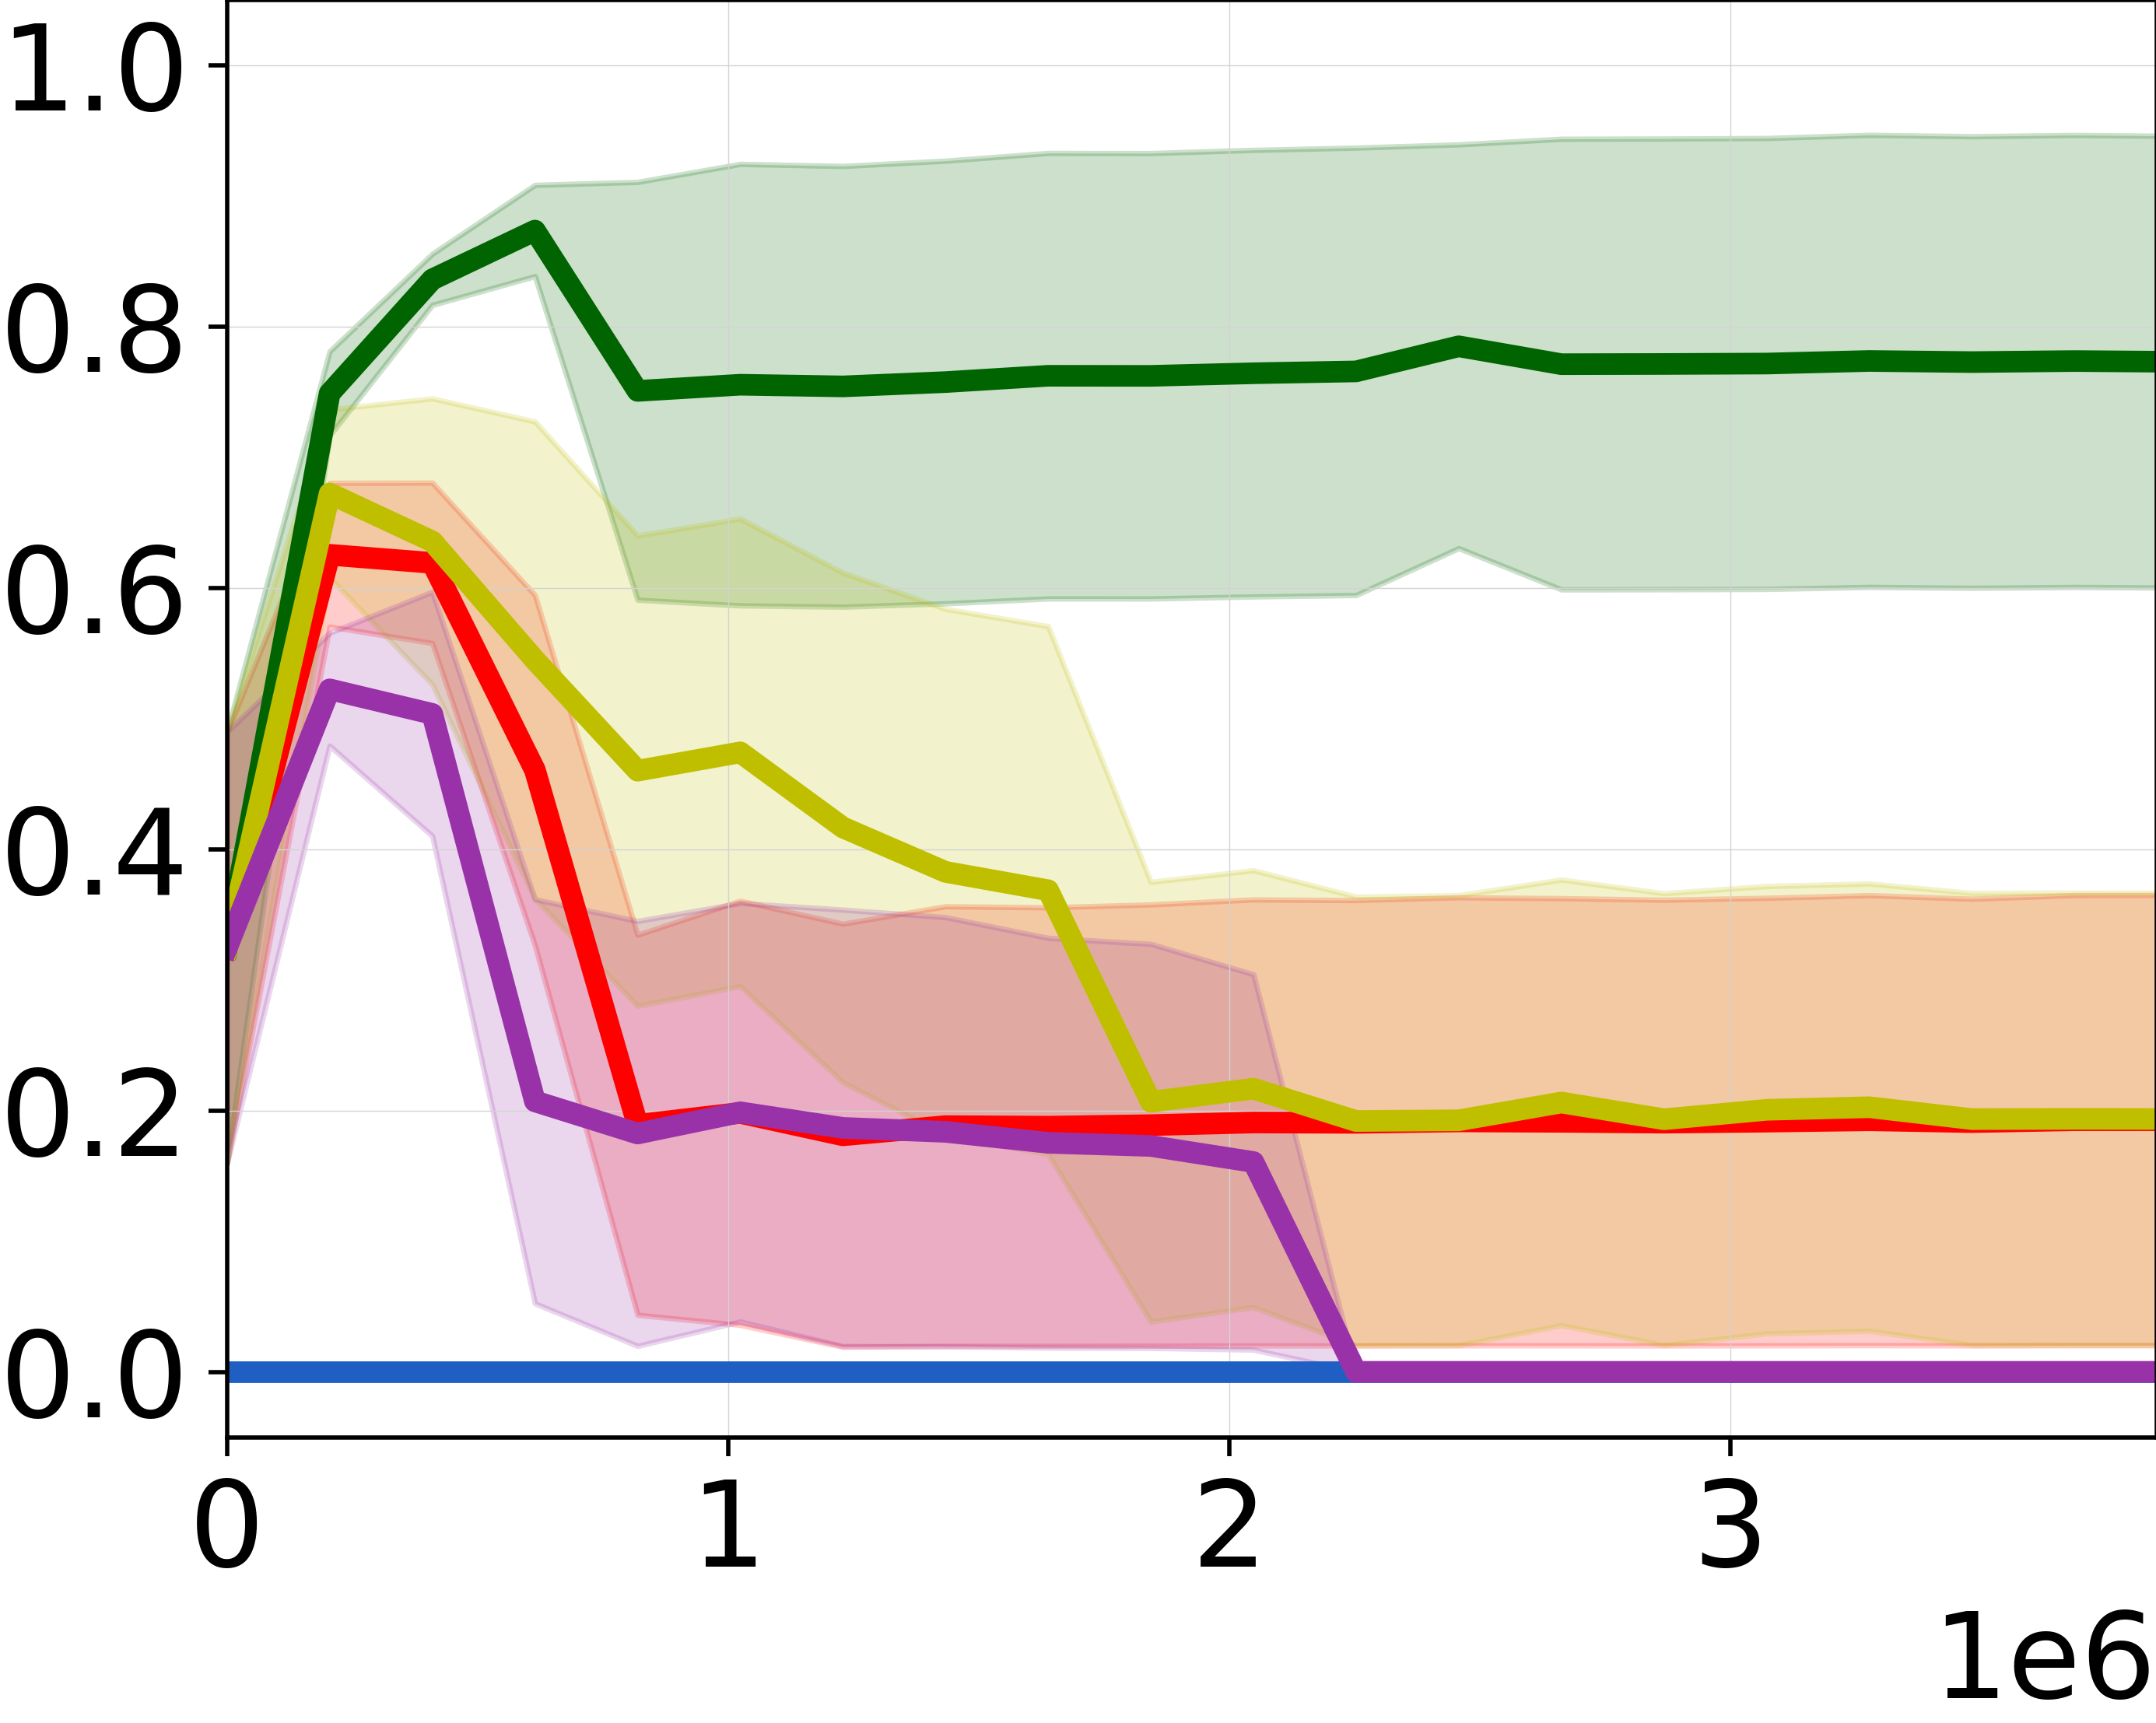
\includegraphics[width=0.18\textwidth]{figures/ablations/is_es/violations.png}}\\
    \subfigure{
\includegraphics[width=0.6\textwidth]{figures/ablations/legend.png}}\\
    \caption{\tiny{Ablation studies on the HalfCheetah environment. All plots were averaged over $5$ seeds. IS refers to importance sampling and ES to early stopping. The x-axis corresponds to the number of timesteps the agent takes in the environment. Shaded regions correspond to the standard error.}}
    \label{fig:abl}
\end{center}
\end{figure}    
\end{frame}


\begin{frame}{Limitations \& Future Work}
\renewcommand{\baselinestretch}{1.5}

\begin{itemize}
    \item Maximum Causal Entropy \& stochastic MDPs.
    \item Soft Constraints. 
    \item Off-policy constraint learning.
    \item Robust imitation learning.
\end{itemize}
\end{frame}

% \begin{frame}[allowframebreaks]{Bibliography}
%     \bibliography{references}
% \end{frame}


\begin{frame}
    \vfill
    \hfill\LARGE{Thank You.}
\end{frame}


\end{document}